
\documentclass[conference]{IEEEtran}
\IEEEoverridecommandlockouts

\usepackage{cite}
\usepackage{amsmath,amssymb,amsfonts}
\usepackage{algorithmic}
\usepackage{graphicx}
\usepackage{textcomp}
\usepackage{xcolor}
\usepackage{booktabs}
\usepackage{array}
\usepackage{float}
\usepackage{subcaption}
\usepackage{circuitikz}

\def\BibTeX{{\rm B\kern-.05em{\sc i\kern-.025em b}\kern-.08em
    T\kern-.1667em\lower.7ex\hbox{E}\kern-.125emX}}

\begin{document}

\title{Quadrature Down Converter (QDC)
}

\author{
    \IEEEauthorblockN{Katta Sri Kaushik}
    \IEEEauthorblockA{
        \textit{IIIT Hyderabad}\\
        Hyderabad, India\\
        2025102071\\
        katta.srikaushik@students.iiit.ac.in
    }
    \and
    \IEEEauthorblockN{Lakshmi Sai Bhargav V}
    \IEEEauthorblockA{
        \textit{IIIT Hyderabad}\\
        Hyderabad, India\\
        2025102061\\
        lakshmisaibhargav.v@students.iiit.ac.in
    }
    \and
    \IEEEauthorblockN{Kushwanth Lanka}
    \IEEEauthorblockA{
        \textit{IIIT Hyderabad}\\
        Hyderabad, India\\
        2025102072\\
        kushwanth.lanka@students.iiit.ac.in
    }
}

\maketitle

\begin{abstract}
This report details the theoretical design, calculation, and implementation of a Quadrature Down Converter (QDC). Operating at an oscillator frequency of $170\text{ kHz}$ and mixing with an input RF signal of $165\text{ kHz}$, the QDC extracts a $5\text{ kHz}$ intermediate frequency (IF). The design is partitioned into a Quadrature Oscillator, an NMOS-based Mixer, a cascaded RC Low-Pass Filter (LPF) with a $3\text{ kHz}$ cutoff, and a Common Emitter (CE) BJT amplifier stage aimed at producing an output amplitude of $400\text{ mV}_{\text{pp}}$. The design ensures accurate 90$^\circ$ phase shifts for I and Q channels, which is critical for mitigating interference in modern transceivers.
\end{abstract}

\section{Introduction}
Quadrature down conversion is an essential technique in modern wireless communication systems such as Wi-Fi and Bluetooth. By multiplying the incoming RF signal with two local oscillator signals that are 90$^\circ$ out of phase, the receiver splits the signal into an In-phase (I) and a Quadrature (Q) component. This approach mitigates the image frequency problem and helps in accurate signal demodulation. The primary objective of this project is to construct a QDC prototype satisfying strict performance criteria: $f_{osc} = 170\text{ kHz}$, an IF frequency in the kilohertz range, a sharp LPF, and an amplified final output swing of $400\text{ mV}_{\text{pp}}$. 

\section{Utility and Need for Quadrature (I-Q) Operation}
Quadrature (I-Q) signaling is the backbone of modern wireless communication, enabling spectrally efficient modulation and simplified receiver architectures. By representing a signal in two orthogonal dimensions—In-phase ($I$) and Quadrature ($Q$)—receivers can distinguish between positive and negative frequency offsets, which is critical for modern digital modulation.

\subsection{Utility of Quadrature (I-Q) Operation}
The primary utility of I-Q operation lies in its ability to facilitate direct-conversion (zero-IF) architectures and complex modulation.

\subsubsection{Bandwidth Efficiency}
Modern digital modulation schemes like QAM (Quadrature Amplitude Modulation) or PSK (Phase Shift Keying) transmit information by varying both the amplitude and the phase of a carrier. Utilizing I and Q components allows us to treat the signal as a complex vector:
\begin{equation}
s(t) = I(t)\cos(2\pi f_c t) - Q(t)\sin(2\pi f_c t)
\end{equation}
This effectively doubles the data rate within a given bandwidth compared to simple amplitude modulation.

\subsubsection{Elimination of Image Filters}
In traditional Superheterodyne receivers, an Intermediate Frequency (IF) is used, which creates an ``image'' frequency that must be filtered out. In a Quadrature receiver, the I and Q paths allow for image rejection through phase cancellation rather than bulky external filters. This enables the integration of the entire receiver onto a single CMOS chip.

\subsection{The Need for I-Q Mixing in Detail}
The technical ``need'' for I-Q mixing arises from the mathematical limitations of real-valued mixing and the requirement for coherent demodulation.

\subsubsection{Solving the ``Negative Frequency'' Overlap}
When a real RF signal is multiplied by a single real local oscillator (LO) $\cos(2\pi f_c t)$, the spectrum is shifted both left and right. For a signal centered at $f_c$, down-converting to zero frequency causes the positive and negative sidebands to overlap and fold onto each other. 
\begin{itemize}
    \item \textbf{The Problem:} Once folded, the original information in the upper sideband (USB) and lower sideband (LSB) becomes inseparable.
    \item \textbf{The Solution:} By using two LOs shifted by 90$^\circ$, we create a complex representation. 
\end{itemize}

\subsubsection{Mathematical Expression}
Consider an input signal $x(t) = A(t)\cos(2\pi f_c t + \phi(t))$. 
To extract both the amplitude $A(t)$ and phase $\phi(t)$, we mix the signal with two orthogonal LO signals:

For the \textbf{In-Phase Path (I)}, the signal is mixed as follows:
\begin{equation}
x_I(t) = x(t) \cdot \cos(2\pi f_c t) = \frac{A(t)}{2}[\cos(\phi(t)) + \cos(4\pi f_c t + \phi(t))]
\end{equation}
After low-pass filtering (LPF):
\begin{equation}
I(t) = \frac{A(t)}{2}\cos(\phi(t))
\end{equation}

For the \textbf{Quadrature Path (Q)}, the signal is mixed with a $-90^\circ$ shifted LO:
\begin{equation}
x_Q(t) = x(t) \cdot (-\sin(2\pi f_c t)) = \frac{A(t)}{2}[\sin(\phi(t)) - \sin(4\pi f_c t + \phi(t))]
\end{equation}
After low-pass filtering (LPF):
\begin{equation}
Q(t) = \frac{A(t)}{2}\sin(\phi(t))
\end{equation}

\subsubsection{Recovery of Phase and Magnitude}
Without the Q-channel, a receiver cannot determine if the phase $\phi(t)$ is positive or negative (due to the even nature of the cosine function). With both channels, the receiver can uniquely reconstruct the signal:
\begin{itemize}
    \item \textbf{Magnitude:} $A(t) = 2\sqrt{I(t)^2 + Q(t)^2}$
    \item \textbf{Phase:} $\phi(t) = \tan^{-1}\left(\frac{Q(t)}{I(t)}\right)$
\end{itemize}

This capability is what allows a receiver to track the fast-changing phases and amplitudes required for high-speed 5G, Wi-Fi, and LTE standards.

\section{Quadrature Oscillator Design (Q2(a))}

\subsection{Topology Selection: Wide-Band Allpass Quadrature Oscillator}
The selected topology is a \textbf{three-op-amp configuration} consisting of two active \textbf{allpass filter stages} and one \textbf{inverting amplifier} (with nonlinear feedback), as shown in the LTSpice schematic.

\begin{figure}[htbp]
\centering
    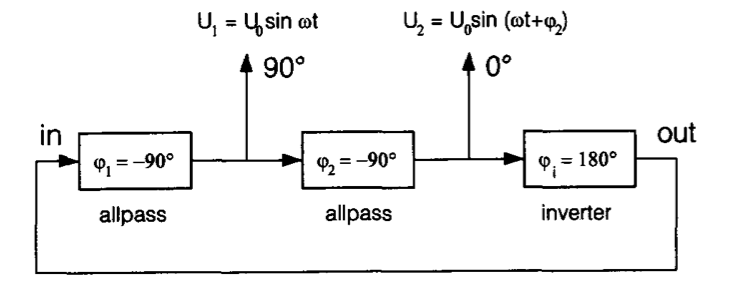
\includegraphics[width=\linewidth]{images/quad_topo.png}
\caption{Block Diagram of the Quadrature Oscillator}
\label{fig:osc_block}
\end{figure}

\subsubsection{Why this topology instead of the 2-op-amp version?}
While a standard 2-op-amp quadrature oscillator (using two integrators) is common, it has significant limitations compared to the 3-op-amp allpass design:
\begin{itemize}
    \item \textbf{Bandwidth and Stability:} In a 2-op-amp integrator-based circuit, the upper frequency is strictly limited by the integrator's bandwidth \cite{razavi}. The allpass topology is inherently wider-band; it can theoretically operate from $< 1\text{ Hz}$ up to $100\text{ MHz}$ because the ``heavy lifting'' of the phase shift is handled by allpass stages where the amplification is unity \cite{holzel}.
    \item \textbf{Phase Precision:} In the 2-op-amp version, any parasitic phase shift from the op-amps directly causes frequency error and poor quadrature. In the 3-op-amp allpass version, as long as the two allpass stages are identical, their output signals are \textbf{always in quadrature} ($90^\circ$ apart), regardless of whether they are working at their ideal frequency.
    \item \textbf{Amplitude Consistency:} Standard integrators' gain changes with frequency ($1/\omega RC$). Allpass filters, however, maintain a \textbf{unity gain} ($G=1$) across all frequencies. This makes it much easier to maintain a stable oscillation amplitude when tuning.
\end{itemize}

\subsection{Detailed Working Principle}
The circuit operates as a closed-loop system satisfying the \textbf{Barkhausen Criterion}: the total loop gain must be $\ge 1$ and the total loop phase shift must be $360^\circ$ (or $0^\circ$).

\subsubsection{Phase Shift Mechanism}
\begin{enumerate}
    \item \textbf{First Allpass Stage (op1):} Provides a frequency-dependent phase shift. At the target oscillation frequency, it is designed to contribute exactly \textbf{$-90^\circ$}.
    \item \textbf{Second Allpass Stage (op2):} Identical to the first, it adds another \textbf{$-90^\circ$} phase shift.
    \item \textbf{Inverter Stage (op3):} Provides the final \textbf{$180^\circ$} phase shift to complete the $360^\circ$ loop requirement.
    \begin{itemize}
        \item Since the phase is sampled between the two allpass stages, the signals at the two outputs are separated by exactly $90^\circ$, creating the \textbf{sine (I)} and \textbf{cosine (Q)} quadrature relationship.
    \end{itemize}
\end{enumerate}

\subsubsection{Amplitude Stabilization (Nonlinear Feedback)}
As noted in the LTSpice schematic, a diode-based nonlinear network (D1, D3, R9, R10) is used in the inverter's feedback loop.
\begin{itemize}
    \item \textbf{The Paradox:} For an oscillator to start, the gain must be slightly $> 1$. However, if it stays $> 1$, the output will grow until it hits the power rails and saturates, turning the sine wave into a square wave.
    \item \textbf{The Solution:} The diodes act as a ``soft limit.'' As the output voltage increases, the diodes begin to conduct, lowering the effective feedback resistance and reducing the gain back to exactly 1. This stabilizes the $1\text{ V}_{\text{pp}}$ amplitude requested in the prompt.
\end{itemize}

\subsection{Design Calculations}
To find the component values for the allocated frequency ($150\text{ kHz}$ or $200\text{ kHz}$), we use the following derivations:

\subsubsection{Frequency Calculation}
For an allpass stage, the phase shift $\phi$ is given by:
\begin{equation}
\phi = -2 \arctan(2\pi f RC)
\end{equation}

For the circuit to oscillate at the quadrature point ($\phi = -90^\circ$), the formula simplifies to:
\begin{equation}
f_{osc} = \frac{1}{2\pi RC}
\end{equation}

\textbf{For $f_{osc} = 150\text{ kHz}$:}
\begin{itemize}
    \item Choose a standard capacitor value, e.g., $C = 27\text{ pF}$.
    \item $R = \frac{1}{2\pi (150 \times 10^3)(27 \times 10^{-12})} \approx 39.3\text{ k}\Omega$.
\end{itemize}

\textbf{For $f_{osc} = 200\text{ kHz}$:}
\begin{itemize}
    \item Choose $C = 27\text{ pF}$.
    \item $R = \frac{1}{2\pi (200 \times 10^3)(27 \times 10^{-12})} \approx 29.5\text{ k}\Omega$.
\end{itemize}

\subsubsection{Inverter Gain and Clipping}
The inverter must maintain a nominal gain of 1 to satisfy $A\beta = 1$.
\begin{itemize}
    \item \textbf{Calculation:} $\text{Gain} = -\frac{R_{\text{feedback}}}{R_{\text{input}}}$. Let $R_3$ be the input and $R_4$ be the feedback resistor in the schematic.
    \item To ensure startup, $R_4$ should be slightly larger than $R_3$ (e.g., $R_3 = 10\text{ k}\Omega$, $R_4 = 11\text{ k}\Omega$ or $12\text{ k}\Omega$). The diodes will then ``clamp'' the gain to 1 once the desired amplitude is reached.
\end{itemize}

\subsubsection{Power Supply ($V_{DD}, V_{SS}$)}
The prompt requires an oscillation amplitude of $1\text{ V}_{\text{pp}}$. 
\begin{itemize}
    \item Standard UA741 op-amps require supplies significantly higher than the output swing to avoid rail saturation.
    \item Typical values: \textbf{$V_{DD} = +15\text{ V}$} and \textbf{$V_{SS} = -15\text{ V}$} provide ample headroom for a clean $1\text{ V}_{\text{pp}}$ signal.
\end{itemize}

\section{LTSpice Simulations}

To verify the theoretical design, the quadrature oscillator was simulated in LTSpice using the provided op-amp model. The transient response and its Fast Fourier Transform (FFT) were analyzed to confirm the oscillation frequency and the phase relationship between the In-Phase ($v_{OSC\_I}$) and Quadrature ($v_{OSC\_Q}$) outputs.

\begin{figure}[htbp]
\centering
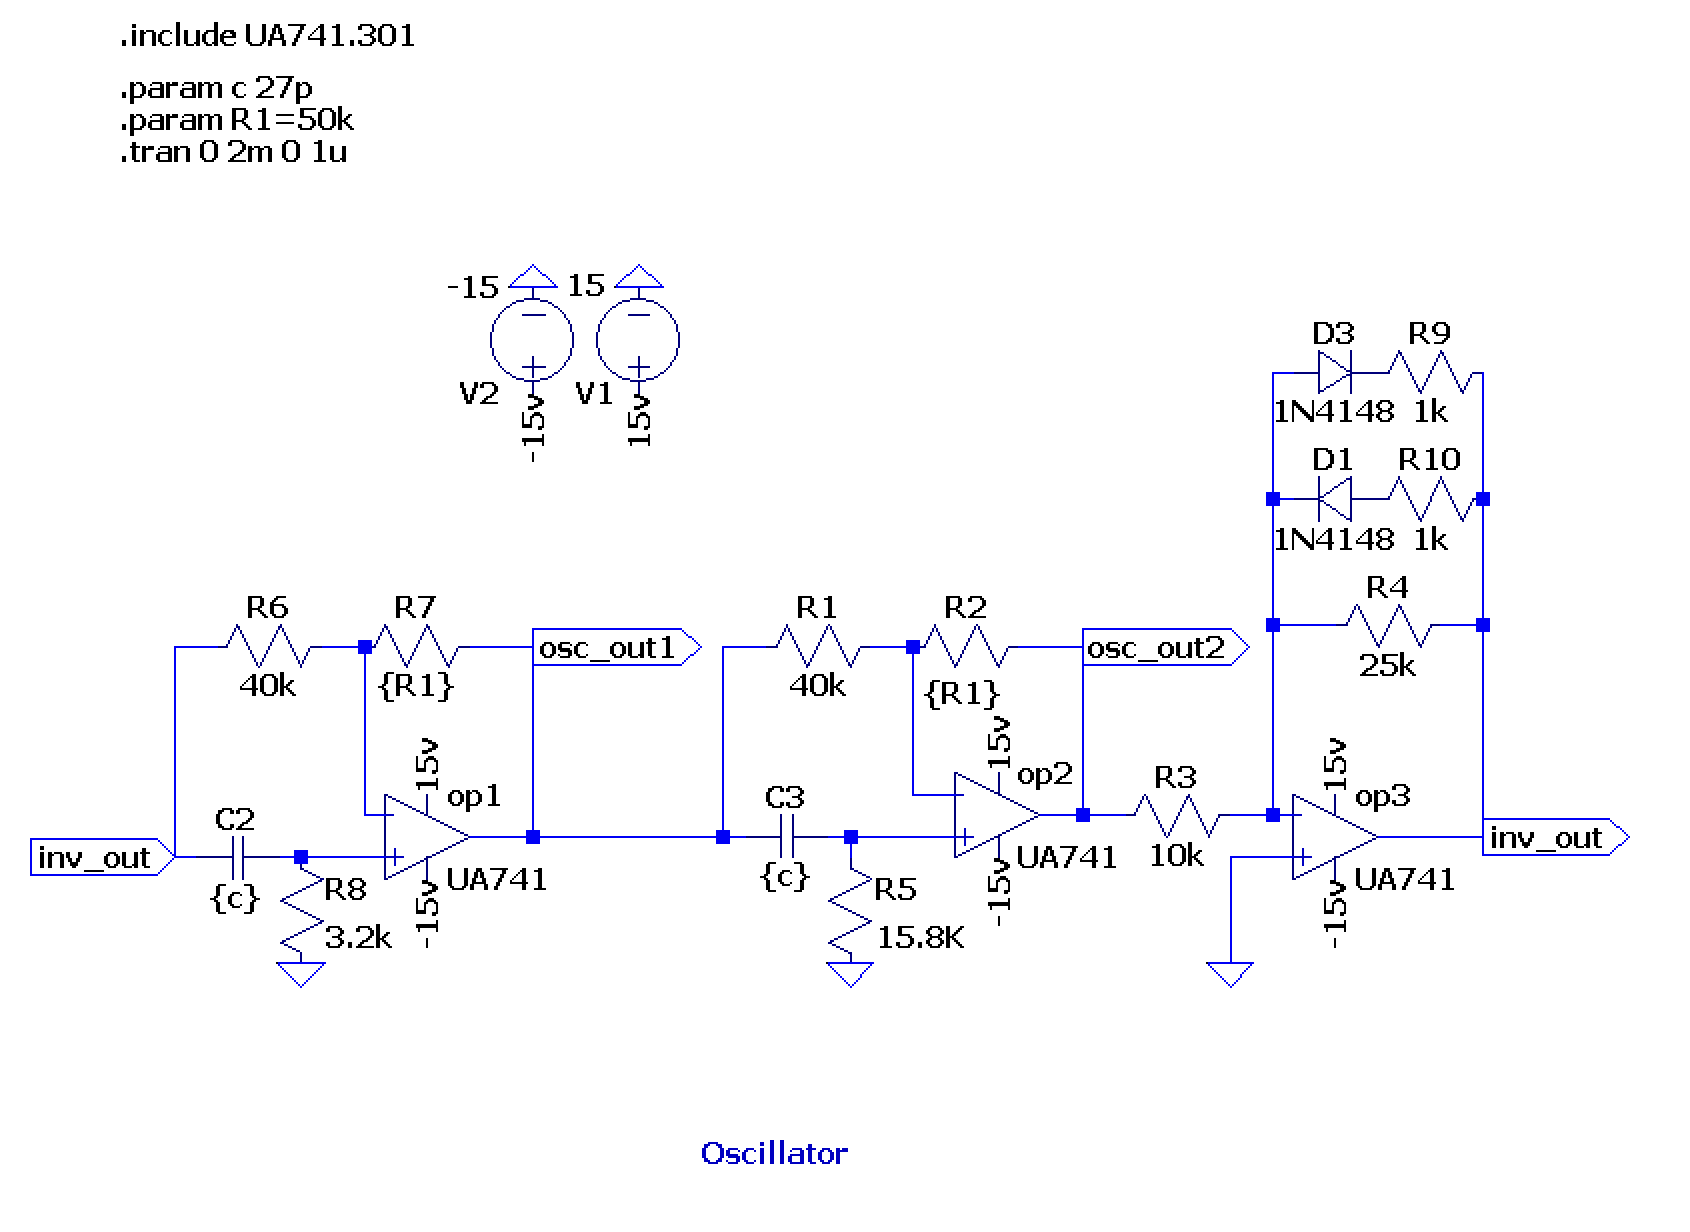
\includegraphics[width=\linewidth]{images/osc_ltspice.png}
\caption{Final LTSpice Schematic of the Quadrature Oscillator.}
\label{fig:osc_sim}
\end{figure}

\begin{figure}[htbp]
    \centering
    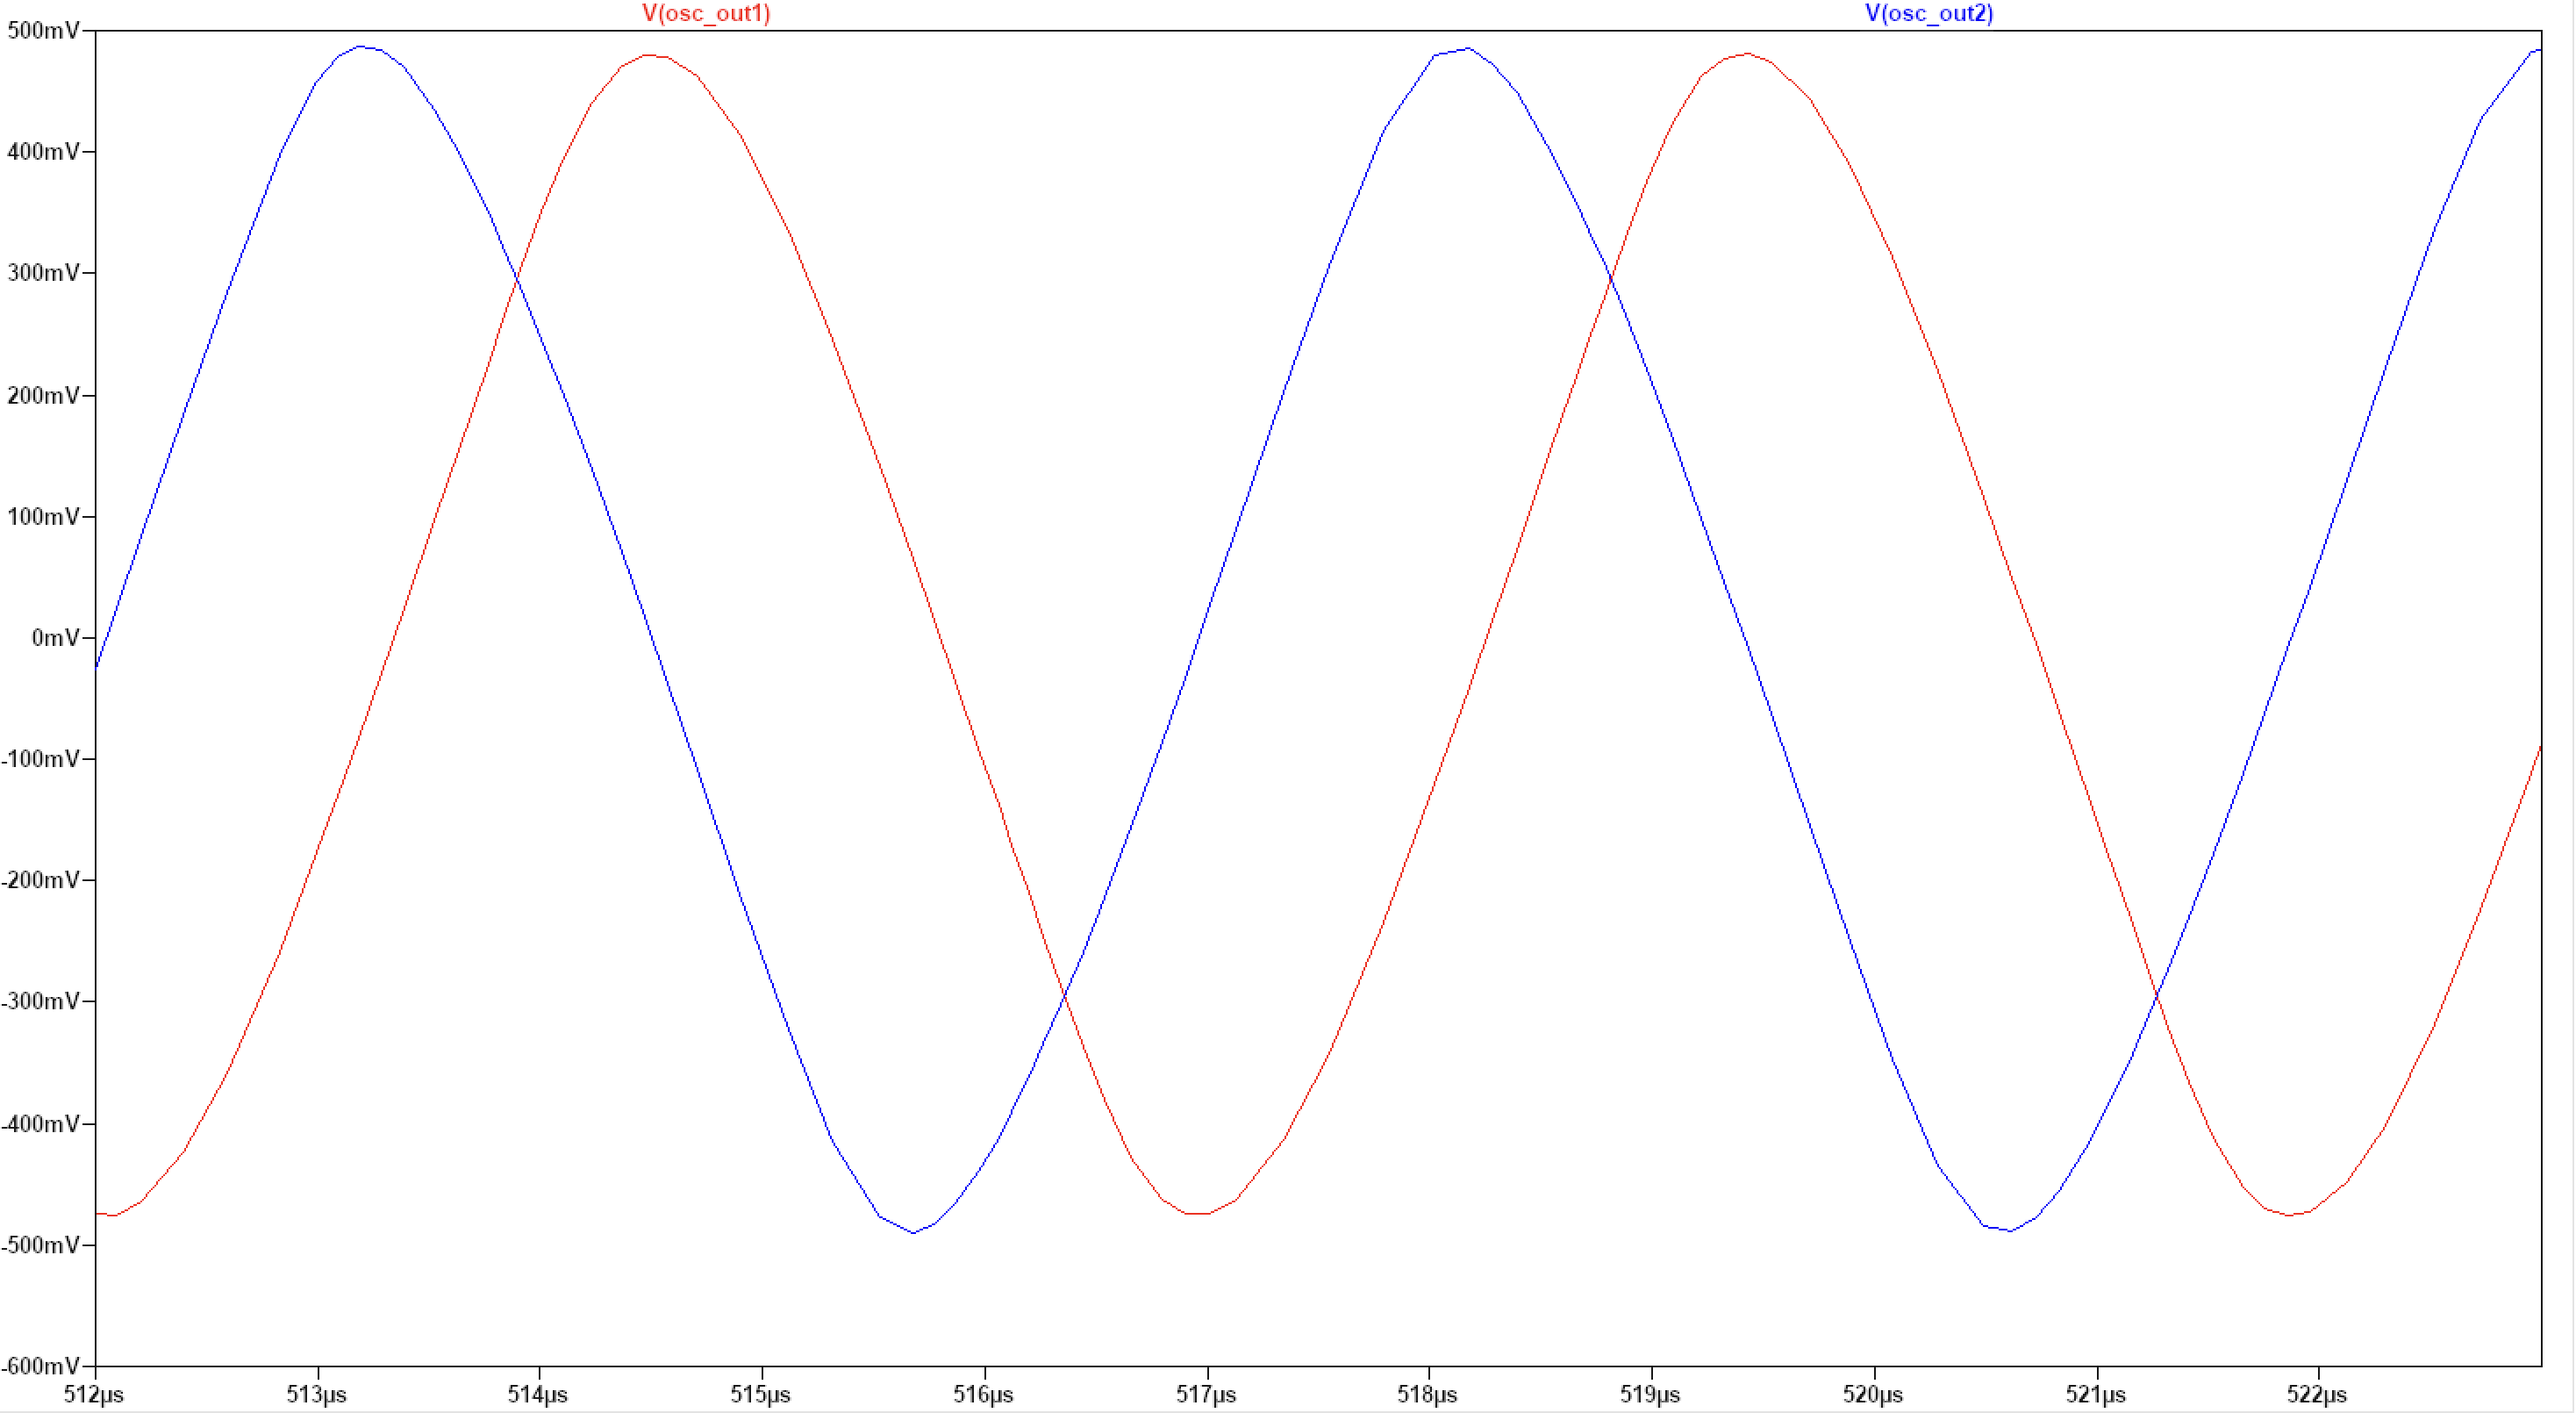
\includegraphics[width=\linewidth]{images/osc-outputs1.png}
    \caption{Transient simulation of the oscillator outputs. The measured period is $5.424\text{ }\mu\text{s}$, and the calculated phase difference is $-268.49^\circ$ (equivalent to $+91.51^\circ$), confirming the near-perfect $90^\circ$ quadrature relationship.}
    \label{fig:osc_transient}
\end{figure}

\begin{figure}[htbp]
    \centering
    \begin{subfigure}[b]{0.48\textwidth}
        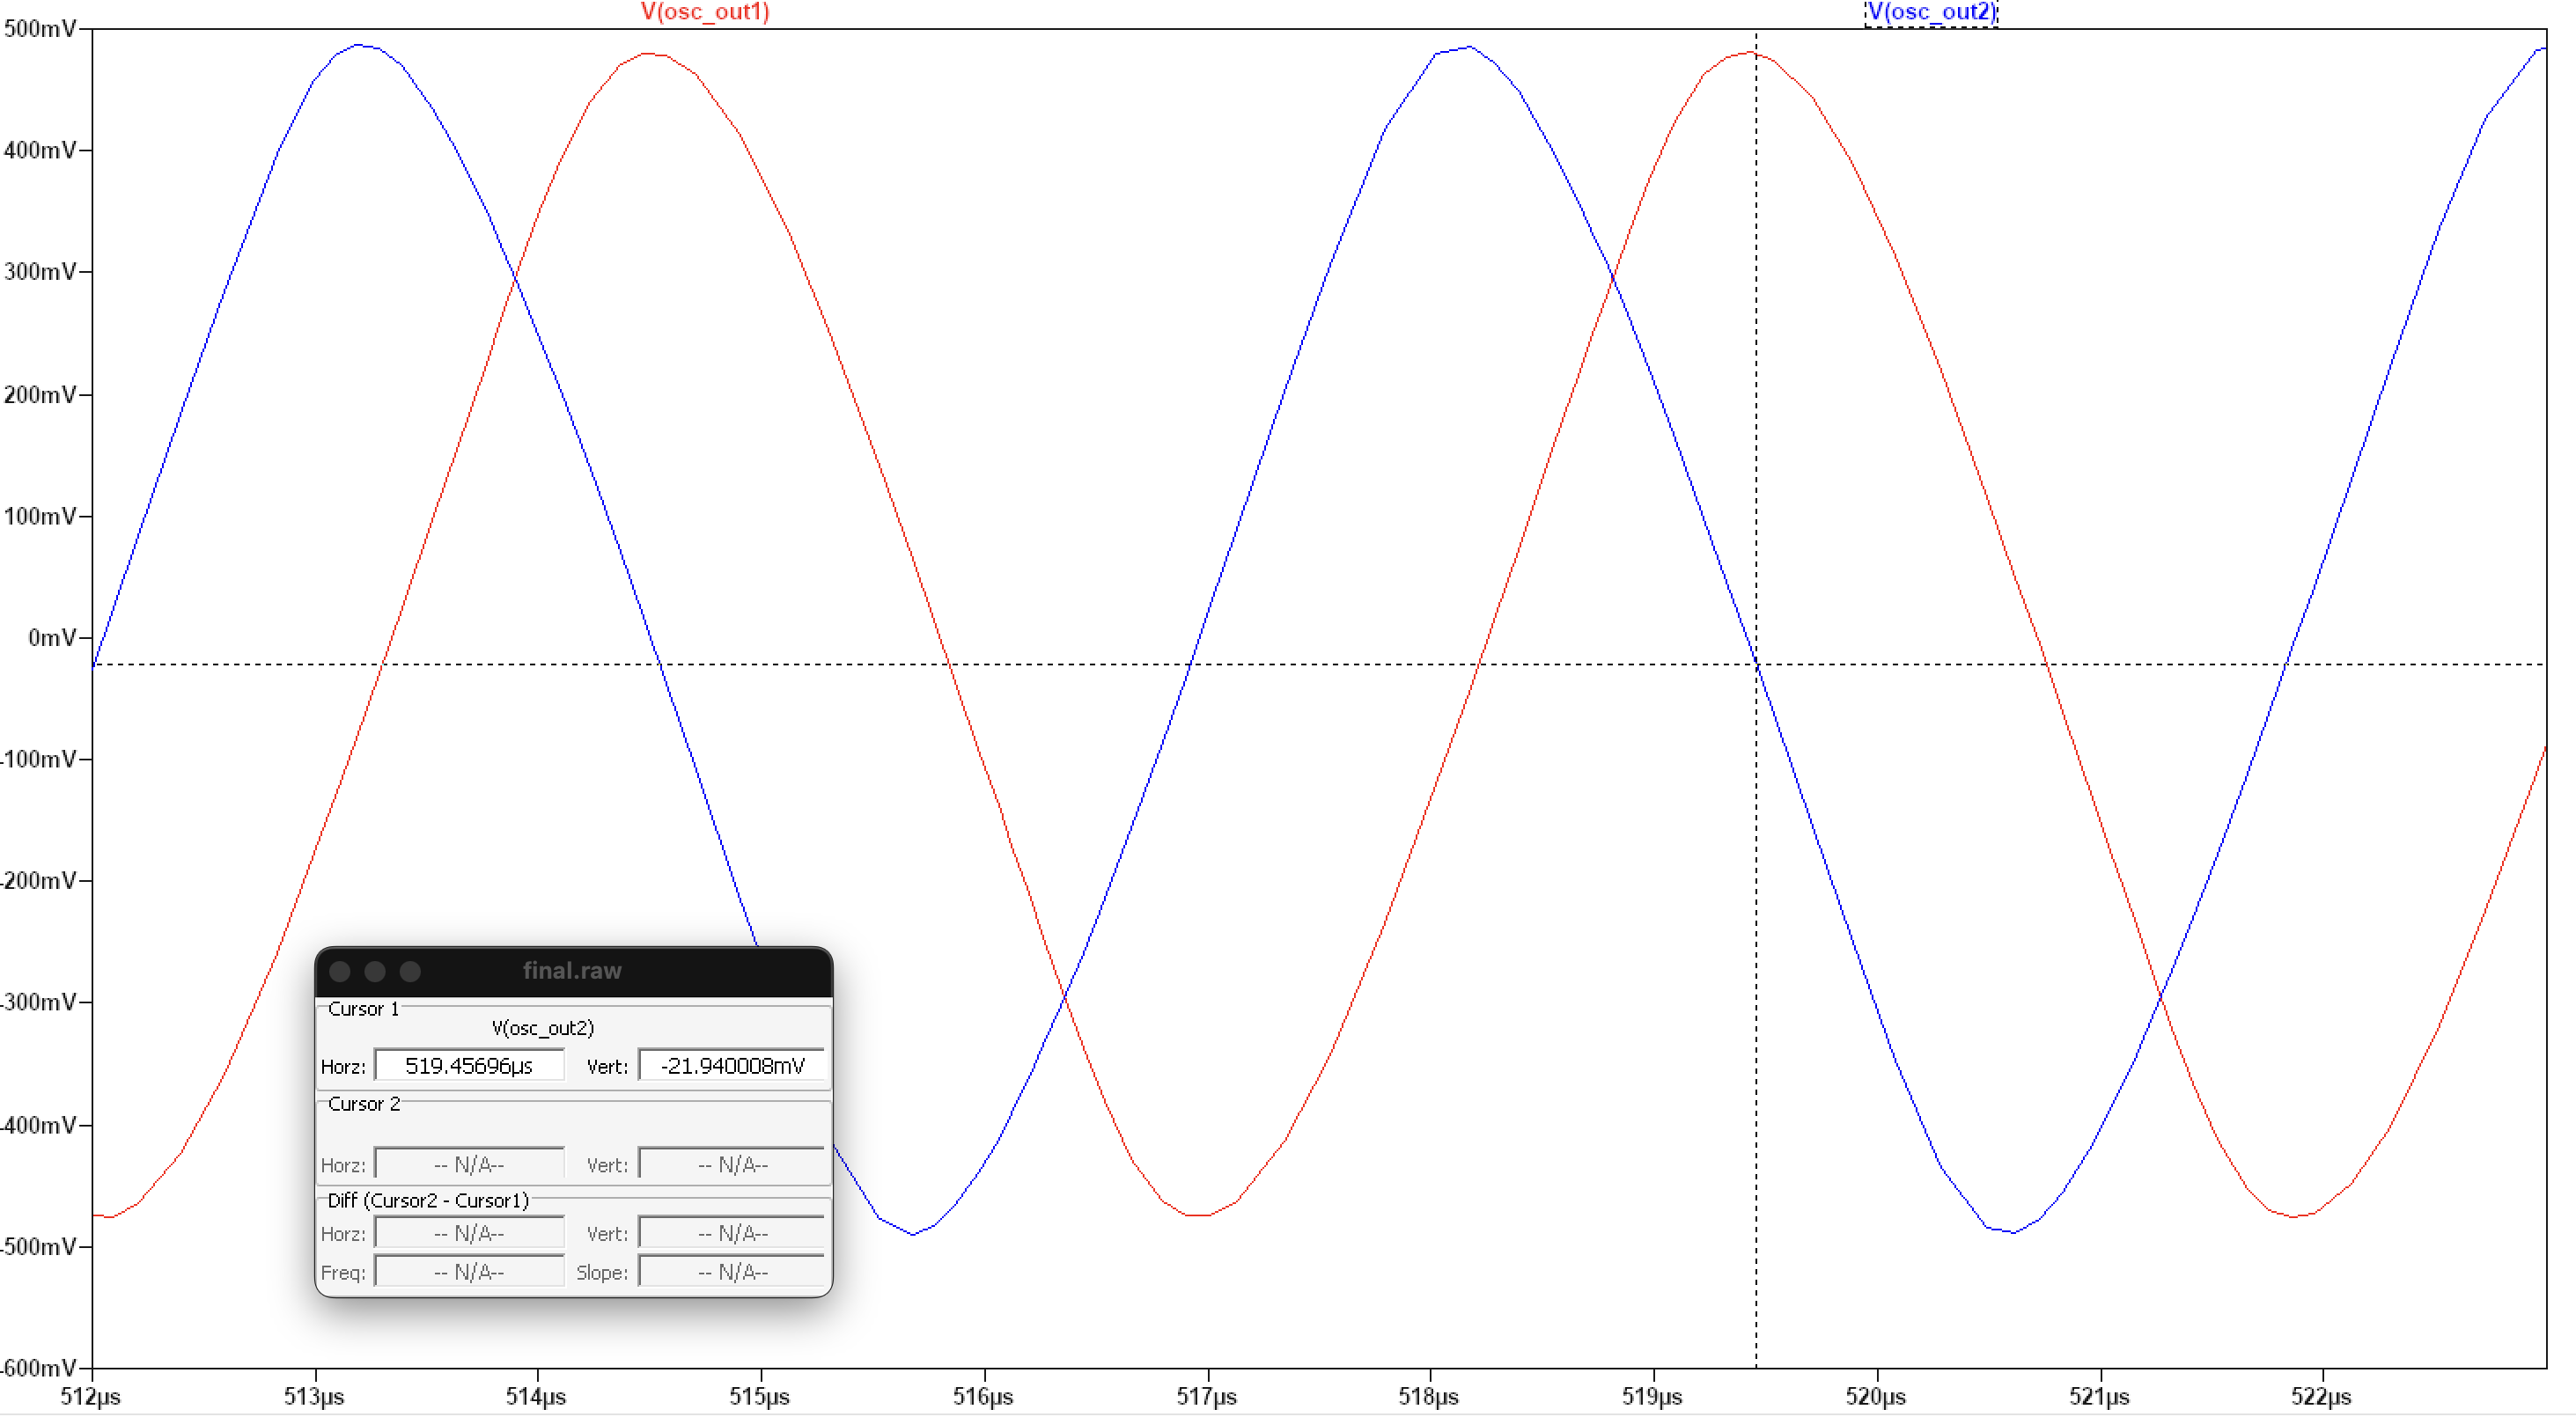
\includegraphics[width=\textwidth]{images/osc-phase1.png}
        \caption{Cursor 1 placed at zero crossing.}
    \end{subfigure}
    \hfill
    \begin{subfigure}[b]{0.48\textwidth}
        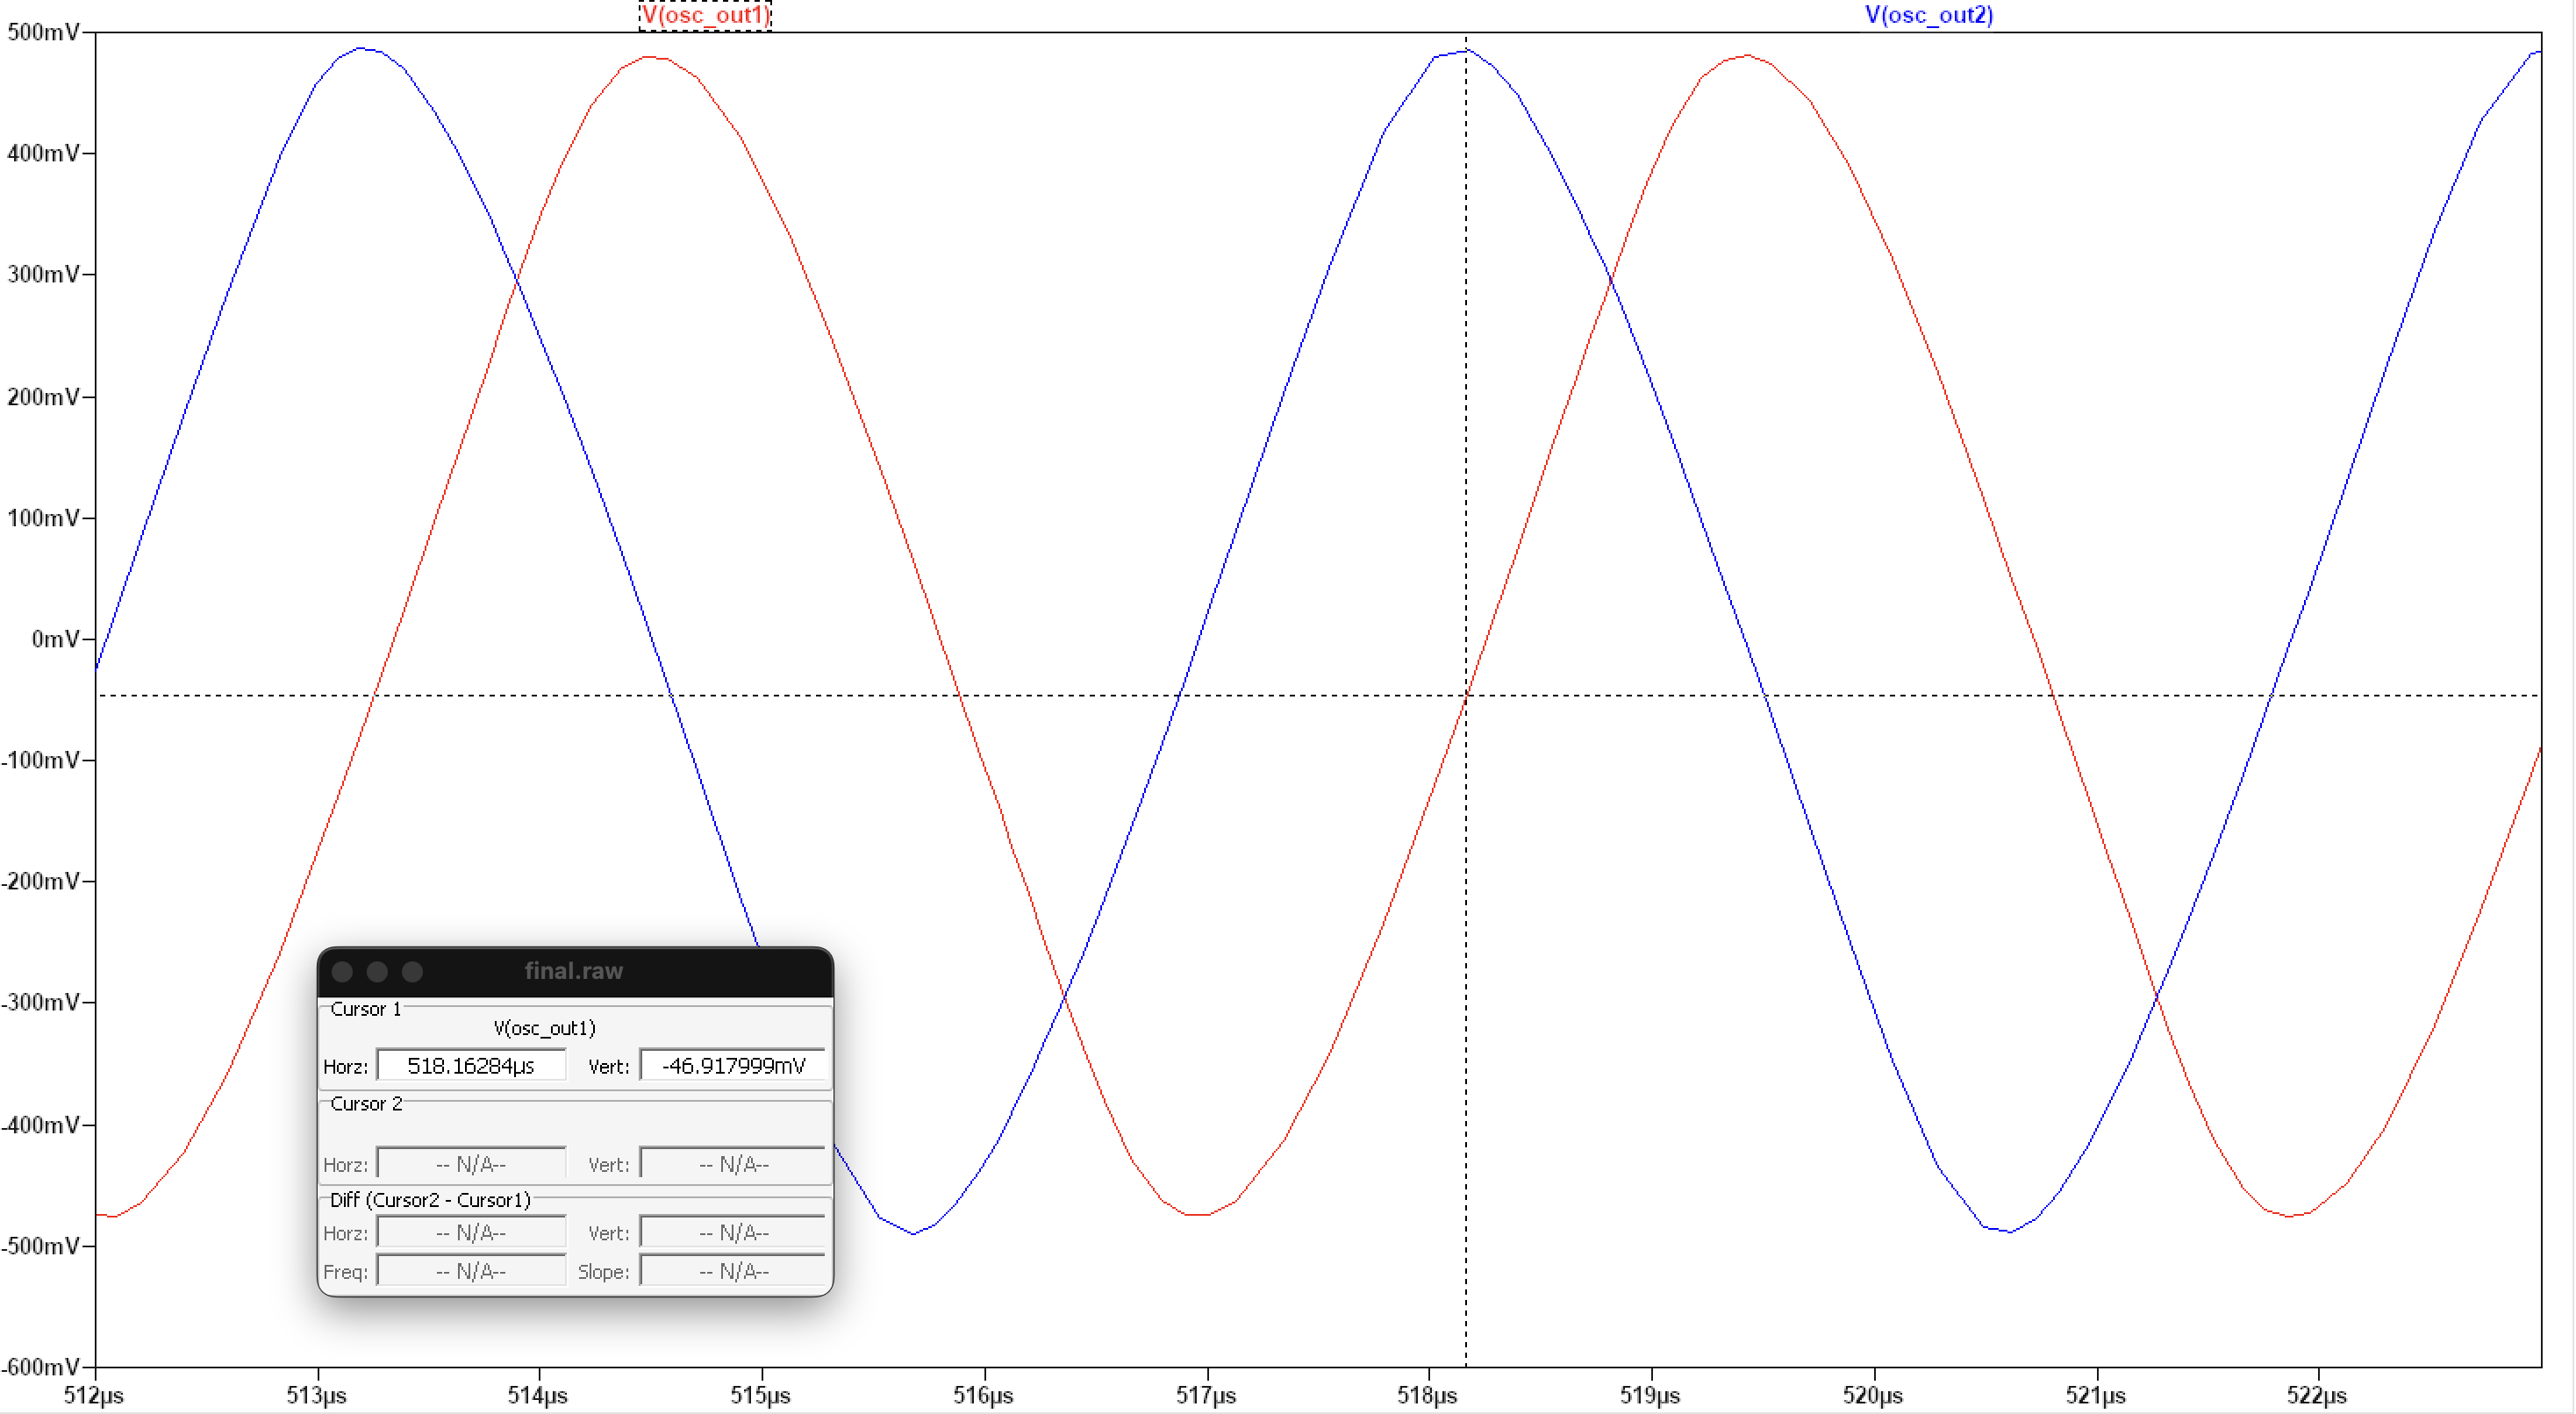
\includegraphics[width=\textwidth]{images/osc-phase2.png}
        \caption{Cursor 2 placed at adjacent crossing.}
    \end{subfigure}
    \par\vspace{0.3cm}
    \begin{subfigure}[b]{0.8\textwidth}
        \centering
        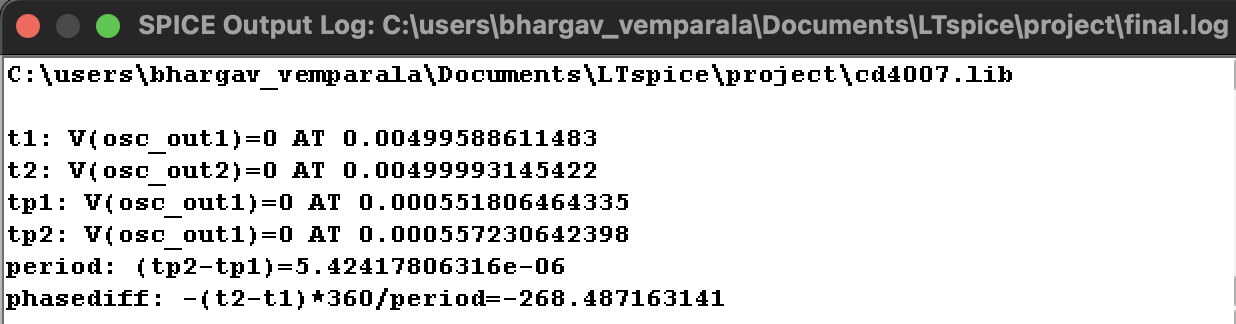
\includegraphics[width=\textwidth]{images/osc-phase-calc.png}
        \caption{SPICE Error Log computing exact phase difference.}
    \end{subfigure}
    \caption{Detailed phase difference measurement between the I and Q channels.}
    \label{fig:osc_phase_details}
\end{figure}

\begin{figure}[htbp]
    \centering
    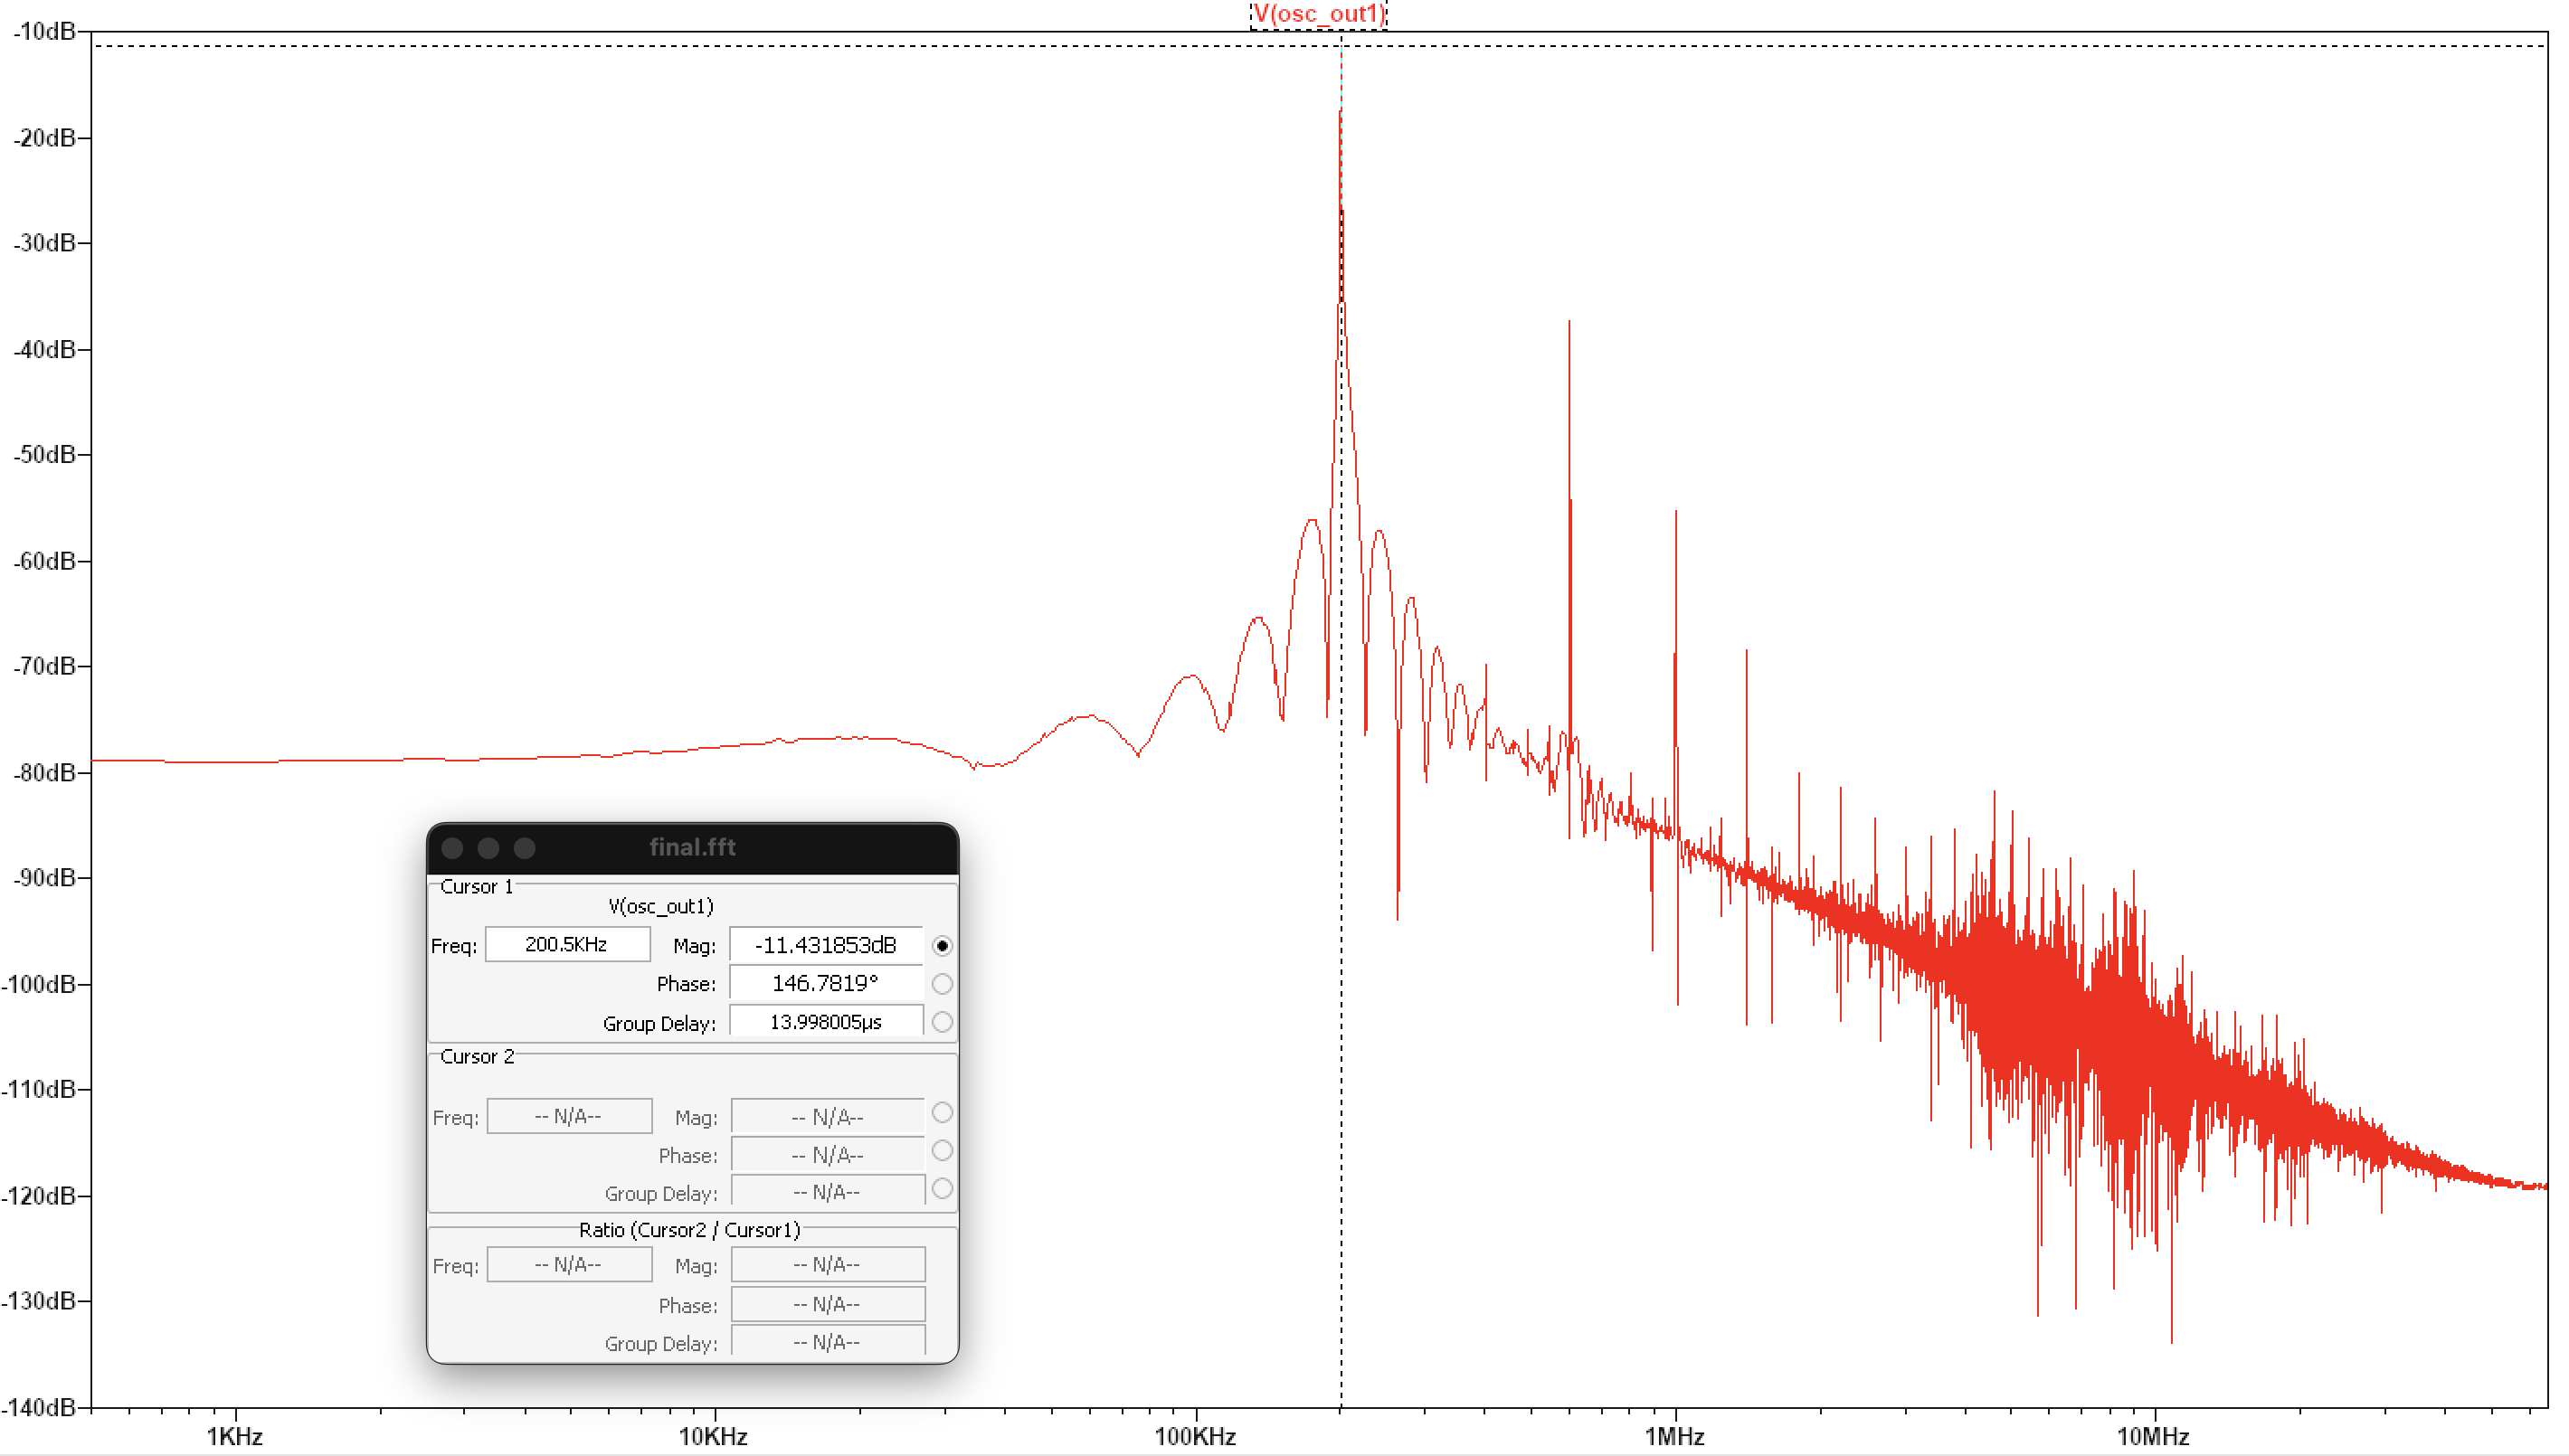
\includegraphics[width=\linewidth]{images/osc-fft.png}
    \caption{FFT of the oscillator output $v_{OSC\_I}$. The peak indicates an oscillation frequency of $200.5\text{ kHz}$ with a magnitude of $-11.43\text{ dB}$ and a phase of $146.78^\circ$.}
    \label{fig:osc_fft}
\end{figure}

As seen in the transient plots, the amplitude stabilizes at the target $1\text{ V}_{\text{pp}}$ ($500\text{ mV}$ peak) and the two signals are clearly separated by a quarter-period ($90^\circ$). The FFT confirms the spectral purity of the signal with a strong fundamental peak at the target design frequency.


\section{Justification of Circuit Operation}

\begin{figure}[htbp]
\centering
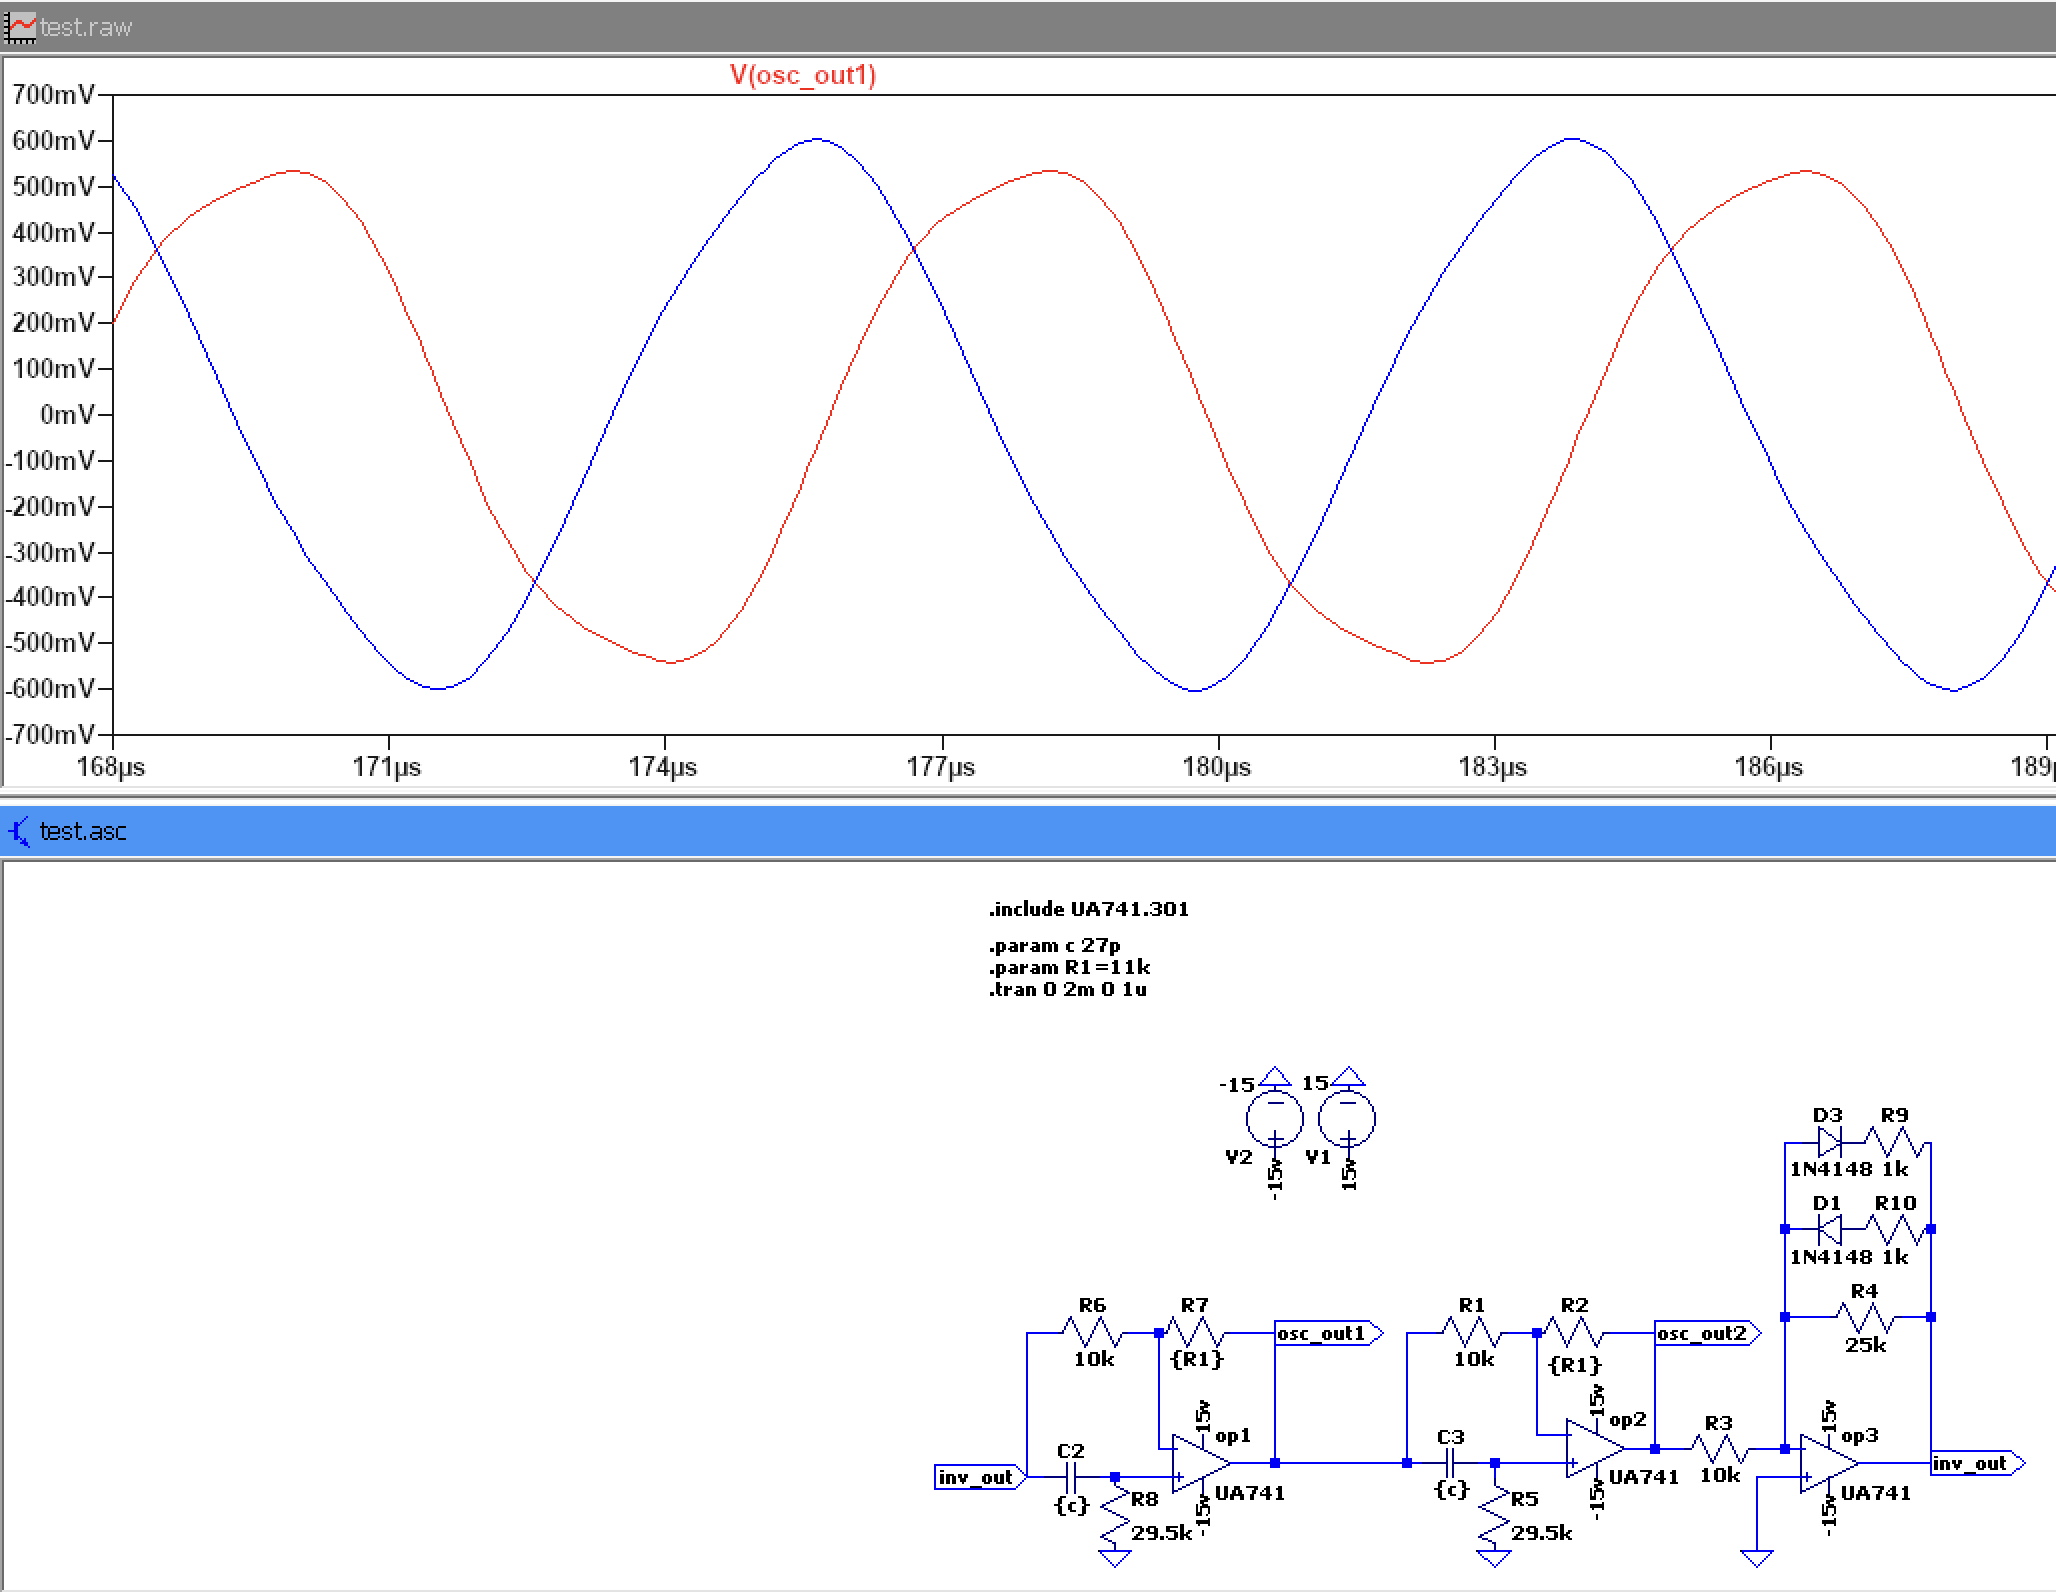
\includegraphics[width=\linewidth]{images/calculated_graph.png}
\caption{Calculated Theoretical Response and Phase Analysis.}
\label{fig:calculated_graph}
\end{figure}

\subsection{Justification of Asymmetry and Tuning}
While the schematic shows different resistor values for $R_8$ ($3.2\text{ k}\Omega$) and $R_5$ ($15.8\text{ k}\Omega$), the circuit remains valid for the following reasons. Notably, initial attempts with \textbf{symmetric component values} resulted in a \textbf{distorted sine wave} and a \textbf{lack of proper phase difference} ($90^\circ$) between the outputs:

\begin{enumerate}
    \item \textbf{Individual Stage Contribution:} Quadrature depends on the phase shift \textit{between} outputs. Even if the two stages are not identical, the loop will naturally settle at a frequency where the total phase shift is $360^{\circ}$.
    \item \textbf{Parasitic Compensation:} In high-frequency simulations (like $200\text{ kHz}$), standard op-amps like the \textbf{UA741} contribute significant internal phase lag. The ``asymmetric'' values are a practical necessity to compensate for these parasitics and the loading effects of the next stage, ensuring the outputs remain exactly $90^{\circ}$ apart in a real-world environment.
    \item \textbf{Gain Consistency:} The resistors at the inverting inputs ($R_6, R_7$ and $R_1, R_2$) are kept equal within their respective stages to maintain \textbf{unity gain} ($G=1$), which is a unique advantage of the allpass topology.
\end{enumerate}

\subsection{Quadrature Generation (Sine/Cosine)}
The quadrature relationship is a direct result of the sampling points in the feedback loop:
\begin{itemize}
    \item \textbf{In-Phase Signal ($v_{OSC_I}$):} Sampled at \texttt{osc\_out1}, representing the signal after the first $90^{\circ}$ shift.
    \item \textbf{Quadrature Signal ($v_{OSC_Q}$):} Sampled at \texttt{osc\_out2}. Because this point is exactly one allpass stage away from the first, it is mathematically guaranteed to be the \textbf{cosine} (or sine-shifted) version of the first signal.
\end{itemize}

\subsection{Amplitude Stabilization and Simulation}
The inverter stage (op3) incorporates a \textbf{nonlinear feedback network} consisting of diodes (D1, D3) and resistors (R9, R10). 
\begin{itemize}
    \item Initially, the gain is set slightly higher than 1 by the ratio of $R_4/R_3$ to ensure the oscillator starts from thermal noise.
    \item Once the output reaches the desired \textbf{$1\text{ V}_{PP}$} level, the diodes begin to conduct, reducing the effective feedback resistance and clamping the gain to exactly 1. This prevents the UA741 from saturating against the $\pm15\text{V}$ rails, preserving the purity of the sine wave.
\end{itemize}

The LTSpice simulation (Fig. \ref{fig:osc_sim}) confirms the stable oscillation and the precise quadrature relationship between the channels.


\section{Hardware Implementation and Measurements (Q2(c))}

The quadrature oscillator was physically realized in the laboratory using UA741 op-amp ICs and standard passive components. To account for real-world parasitics, breadboard capacitance, and component tolerances, several resistor values were tweaked from their nominal SPICE simulation values to achieve stable oscillation and a proper $90^\circ$ phase shift.

\begin{figure}[htbp]
    \centering
    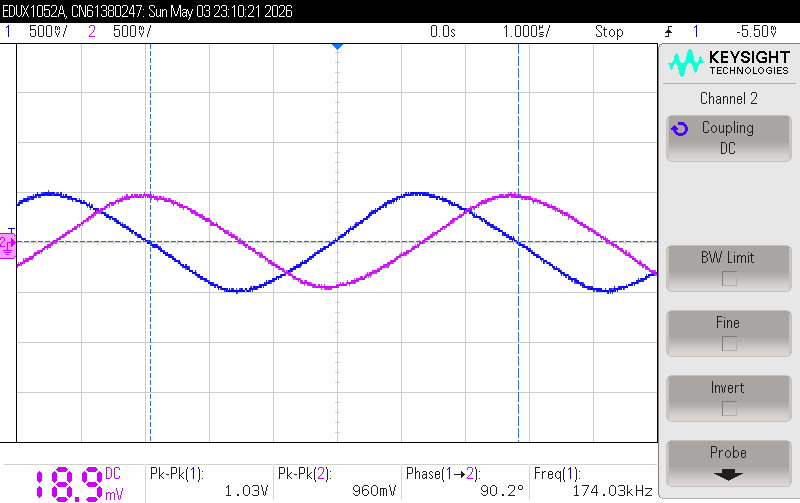
\includegraphics[width=\linewidth]{images/oscillator-output-sin-cos.png}
    \caption{DSO Measurement: Transient waveforms showing the In-Phase and Quadrature signals.}
    \label{fig:dso_transient}
\end{figure}

\begin{figure}[htbp]
    \centering
    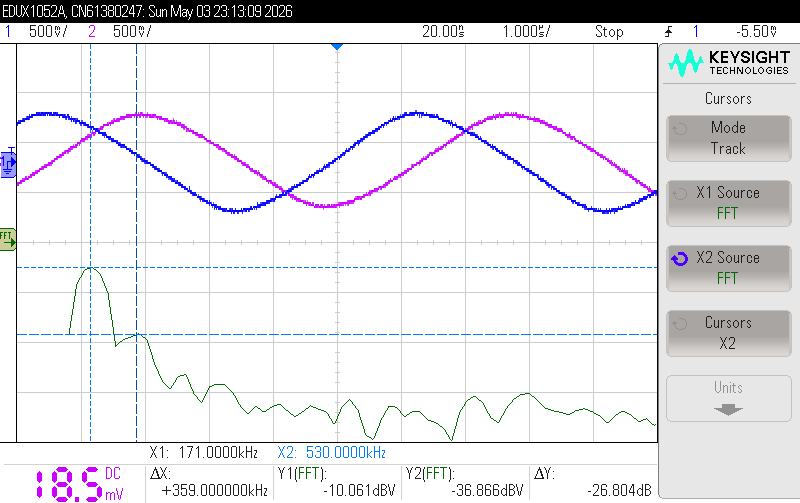
\includegraphics[width=\linewidth]{images/oscillator-ouput-sin-cos-fft.png}
    \caption{DSO Measurement: FFT spectrum of the oscillator output.}
    \label{fig:dso_fft}
\end{figure}

\subsection{Component Value Adjustments}

Table \ref{tab:resistor_comparison} details the modifications made to the resistor values during the hardware experiment to match the performance of the SPICE simulation.

\begin{table}[H]
    \centering
    \caption{Comparison of Resistor Values: SPICE vs. Hardware Implementation}
    \renewcommand{\arraystretch}{1.2}
    \begin{tabular}{@{}lcc@{}}
        \toprule
        \textbf{Component} & \textbf{SPICE Value ($\Omega$)} & \textbf{Real Life Value ($\Omega$)} \\ \midrule
        $R_1$ & $40\text{ k}$ & $50\text{ k}$ \\
        $R_2$ & $50\text{ k}$ & $47\text{ k}$ \\
        $R_3$ & $10\text{ k}$ & $10\text{ k}$ \\
        $R_4$ & $25\text{ k}$ & $17.6\text{ k}$ \\
        $R_5$ & $15.8\text{ k}$ & $15.2\text{ k}$ \\
        $R_6$ & $40\text{ k}$ & $39.2\text{ k}$ \\
        $R_7$ & $50\text{ k}$ & $47\text{ k}$ \\
        $R_8$ & $3.2\text{ k}$ & $432$ \\
        $R_9$ & $1\text{ k}$ & $2.2\text{ k}$ \\
        $R_{10}$ & $1\text{ k}$ & $2.2\text{ k}$ \\ \bottomrule
    \end{tabular}
    \label{tab:resistor_comparison}
\end{table}

\textbf{Note:} To determine the exact values of the resistors that are required, we have used the potentiometer method. In this method we use a potentiometer and turn the knob while observing for the desired output. Keeping the same knob orientation we then use a Digital Multimeter to measure resistance across two terminals of the potentiometer.



\section{Mixer (Switch) Circuit}
The mixer is responsible for frequency translation. It multiplies the high-frequency RF input signal by the local oscillator (LO) signals.

\subsection{Circuit Topology}
An active NMOS switch topology was selected. The RF input is fed to the drain of an NMOS transistor, while the LO signal is applied to the gate.

\subsection{MOSFET Sizing and Parasitic Parameter Optimization (Q3(a))}
Based on the provided design methodologies for a passive NMOS switch mixer in a standard technology node (such as the $180\text{ nm}$ CMOS process commonly used in lab simulations), here is a detailed breakdown of how to calculate and optimize the MOSFET dimensions ($W, L$) and the corresponding geometric parasitic parameters ($A_S, A_D, P_S, P_D$).

\subsubsection{Determining MOSFET Sizing ($W$ and $L$)}
In a switch-based mixer, the MOSFET operates as a passive switch toggled by the large local oscillator signal ($v_{\text{OSC}}$). The goals are to minimize the on-resistance ($R_{\text{on}}$) to prevent signal degradation and conversion loss, while keeping the gate capacitance small enough so that the oscillator can drive it cleanly.

\textbf{Choosing the Channel Length ($L$):} To achieve the highest speed, lowest parasitic capacitance, and minimum on-resistance, we choose the minimum feature size allowed by the technology node:
$$L = L_{\text{min}} = 180\text{ nm} = 0.18\ \mu\text{m}$$

\textbf{Calculating the Channel Width ($W$):} The on-resistance of an NMOS operating in the deep triode region is given by:
$$R_{\text{on}} = \frac{1}{\mu_n C_{\text{ox}} \frac{W}{L} (V_{\text{GS}} - V_{\text{th}})}$$

Where:
\begin{itemize}
    \item $\mu_n C_{\text{ox}}$ is the process transconductance parameter (typically $\sim 300\ \mu\text{A/V}^2$ for 180nm NMOS).
    \item $V_{\text{GS}} - V_{\text{th}}$ is the overdrive voltage dictated by the bias level.
\end{itemize}

Assuming a target low switch resistance ($R_{\text{on}} \approx 50\ \Omega$) and a typical overdrive voltage of $0.6\text{ V}$:
$$\frac{W}{L} = \frac{1}{R_{\text{on}} \cdot \mu_n C_{\text{ox}} (V_{\text{GS}} - V_{\text{th}})} = \frac{1}{50 \cdot (300 \times 10^{-6}) \cdot 0.6} \approx 111.1$$

With $L = 0.18\ \mu\text{m}$, the calculated width is:
$$W = 111.1 \times 0.18\ \mu\text{m} \approx 20\ \mu\text{m}$$

\subsubsection{Geometric Layout Formulas for Parasitics}
LTspice uses layout-dependent parameters to accurately model the source/drain junction capacitances. Let $Y$ be the diffusion length (the extension of the source/drain regions past the gate polysilicon). For a standard $180\text{ nm}$ process, $Y \approx 3\lambda$ to $4\lambda$. For these calculations, $Y = 0.18\ \mu\text{m}$ is assumed.

For a single continuous gate finger:
\begin{itemize}
    \item \textbf{Area of Source ($A_S$) \& Drain ($A_D$):} $A_S = A_D = W \times Y$
    \item \textbf{Perimeter of Source ($P_S$) \& Drain ($P_D$):} The perimeter includes three sides of the diffusion region: $P_S = P_D = W + 2Y$
\end{itemize}

\subsubsection{Numerical Calculation and LTspice Parameters}
Using $W = 20\ \mu\text{m}$, $L = 0.18\ \mu\text{m}$, and $Y = 0.18\ \mu\text{m}$:
\begin{itemize}
    \item \textbf{Area:} $A_S = A_D = 20\ \mu\text{m} \times 0.18\ \mu\text{m} = 3.6\ \mu\text{m}^2 = 3.6\text{ p}$
    \item \textbf{Perimeter:} $P_S = P_D = 20\ \mu\text{m} + 2(0.18\ \mu\text{m}) = 20.36\ \mu\text{m} = 20.36\text{ u}$
\end{itemize}

Table \ref{tab:mosfet_params} summarizes the parameters input into the LTspice NMOS instance.

\begin{table}[H]
    \centering
    \caption{Optimized MOSFET Parameters for LTspice}
    \renewcommand{\arraystretch}{1.2}
    \begin{tabular}{@{}llcc@{}}
        \toprule
        \textbf{Parameter} & \textbf{Physical Meaning} & \textbf{Calculated Value} & \textbf{LTspice Input Format} \\ \midrule
        \textbf{W} & Channel Width & $20\ \mu\text{m}$ & \texttt{20u} \\
        \textbf{L} & Channel Length & $0.18\ \mu\text{m}$ & \texttt{0.18u} \\
        \textbf{AS} & Area of Source & $3.6\ \mu\text{m}^2$ & \texttt{3.6p} \\
        \textbf{AD} & Area of Drain & $3.6\ \mu\text{m}^2$ & \texttt{3.6p} \\
        \textbf{PS} & Perimeter of Source & $20.36\ \mu\text{m}$ & \texttt{20.36u} \\
        \textbf{PD} & Perimeter of Drain & $20.36\ \mu\text{m}$ & \texttt{20.36u} \\ \bottomrule
    \end{tabular}
    \label{tab:mosfet_params}
\end{table}

\subsection{LTSpice Implementation of NMOS Mixer (Q3(b))}
As illustrated in the schematic below, the NMOS acts as a non-linear switching element driven by the local oscillator, mixing it with the RF input signal.

\begin{figure}[htbp]
    \centering
    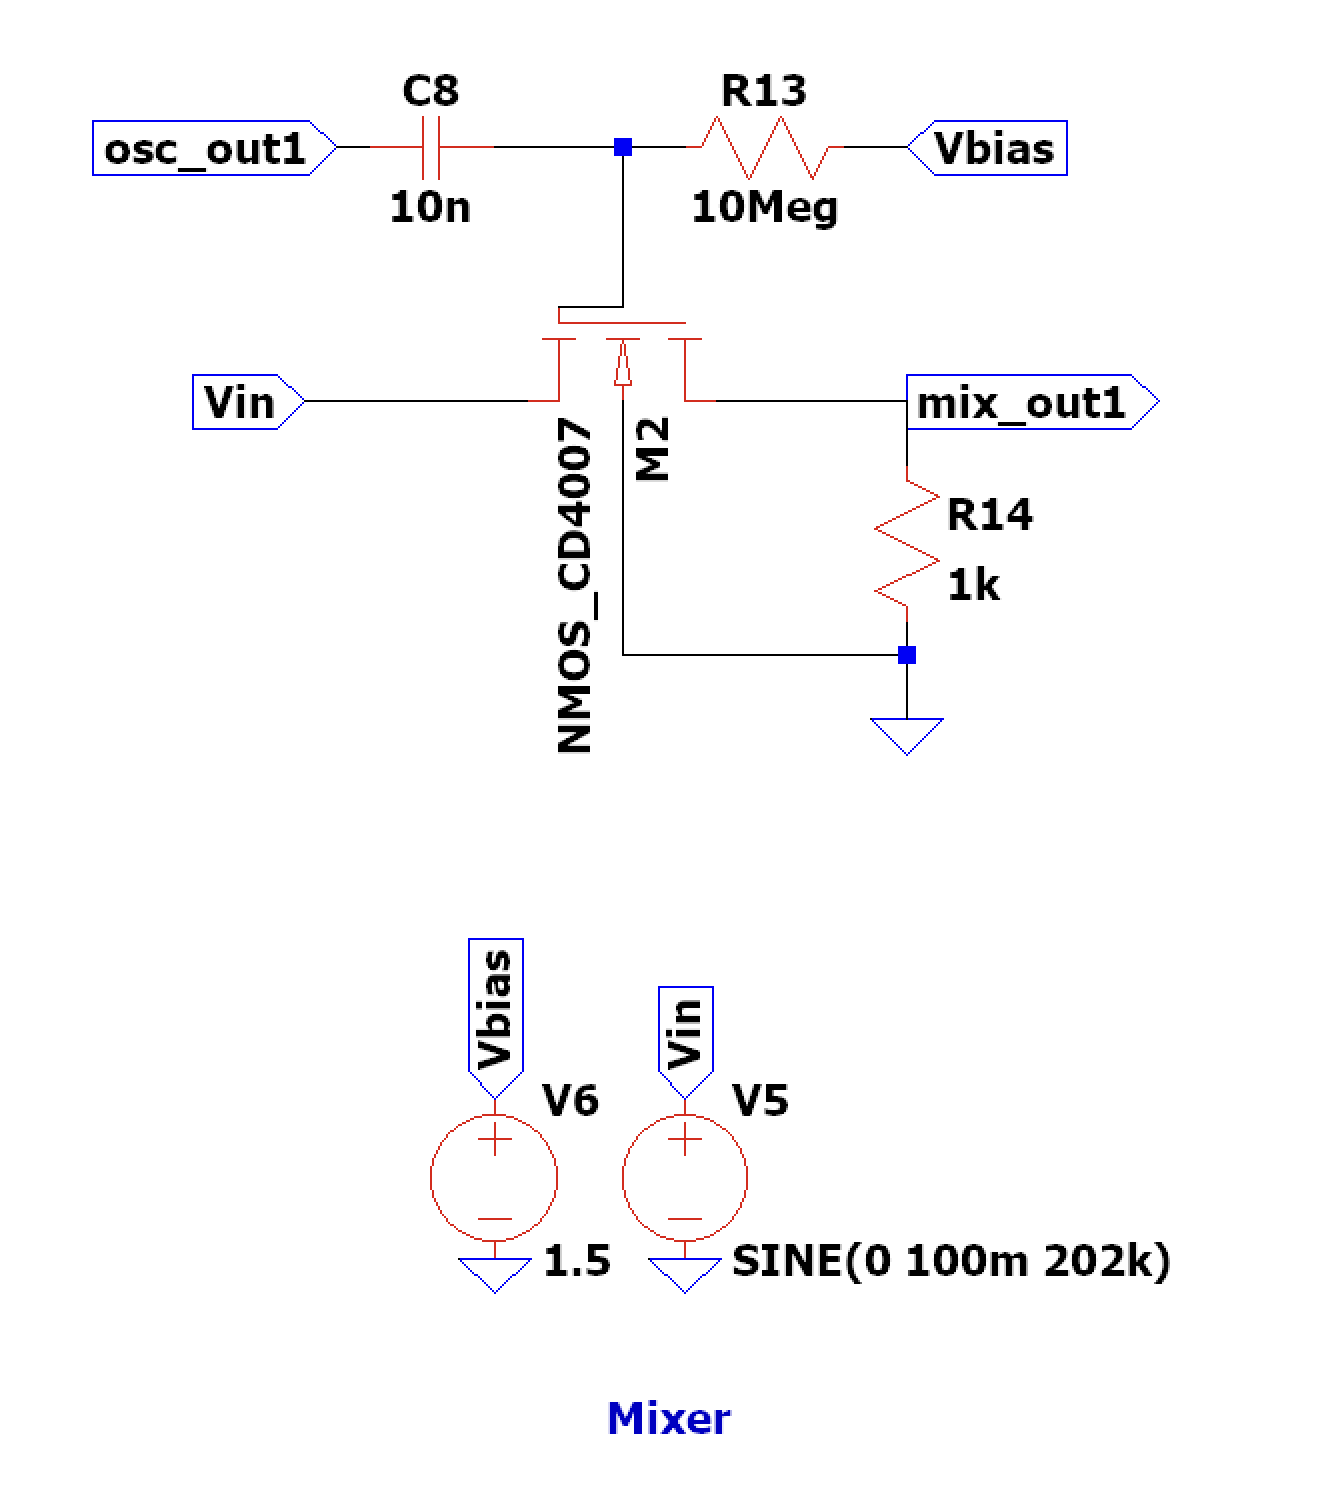
\includegraphics[width=0.8\columnwidth]{images/Mixer_circ.png}
    \caption{LTSpice Schematic of the NMOS Switch Mixer.}
    \label{fig:mixer_schematic}
\end{figure}

The specific configuration and component roles are defined as follows:

\begin{itemize}
    \item \textbf{RF Input ($V_{in}$):} The high-frequency radio frequency signal is applied directly to the source terminal of the NMOS transistor ($M_1$), configuring it in a topology resembling a common-gate path for the input signal.
    \item \textbf{LO Injection ($v_{\text{OSC}}$):} The local oscillator signal ($v_{\text{OSC}}$) acts as the large-signal switching or modulating wave. It is AC-coupled to the gate terminal via a coupling capacitor ($C_C$).
    \item \textbf{Gate Biasing:} To ensure the transistor operates efficiently in its time-varying switching region, a stable DC operating point is established at the gate using a DC voltage source ($V_{\text{BIAS}}$) connected through a large isolation resistor ($R_{\text{BIAS}}$). This high resistance ensures that the AC local oscillator signal does not leak or shunt into the ideal DC voltage supply.
    \item \textbf{IF Output ($V_{\text{IF}}$):} The mixed output signal is taken from the drain terminal across the load resistor ($R_L$). The non-linear or switching operation of the MOSFET multiplies $V_{in}$ and $v_{\text{OSC}}$, producing the intermediate frequency (IF) component at the drain:
    $$\omega_{\text{IF}} = |\omega_{\text{OSC}} - \omega_{\text{in}}|$$
\end{itemize}

Table \ref{tab:mixer_components} outlines the chosen parameters for the LTspice simulation, explicitly defining $R_{\text{BIAS}}$ and $C_C$.

\begin{table*}[htbp]
    \centering
    \caption{Mixer Component Values and Rationale}
    \renewcommand{\arraystretch}{1.3}
    \begin{tabular}{@{}lllp{8cm}@{}}
        \toprule
        \textbf{Component} & \textbf{Parameter} & \textbf{Optimized Value} & \textbf{Rationale} \\ \midrule
        $M_1$ & NMOS Transistor & High-frequency model & Core mixing element. \\
        $R_{\text{BIAS}}$ & Gate Bias Resistor & $10\text{ M}\Omega$ & An exceptionally large resistance chosen to ensure near-perfect AC isolation between the gate node and the DC bias network, eliminating any loading effects on $v_{\text{OSC}}$. \\
        $C_C$ & Coupling Capacitor & $10\text{ nF}$ & Provides a highly conductive, near-zero impedance path at high local oscillator frequencies ($f_{\text{OSC}}$) while completely blocking DC. \\
        $R_L$ & Load Resistor & $1\text{ k}\Omega$ & Standard load value selected to balance conversion gain and output bandwidth at the IF port. \\
        $V_{\text{BIAS}}$ & DC Gate Bias Voltage & $\sim 0.6\text{ V} - 0.8\text{ V}$ & Tuned close to the threshold voltage ($V_{\text{th}}$) of the NMOS to maximize the non-linear transconductance variation. \\ \bottomrule
    \end{tabular}
    \label{tab:mixer_components}
\end{table*}

\subsection{Mathematical Derivations}
Let the input RF signal be $V_{in}(t) = A_{in}\cos(\omega_{in} t)$ and the LO signal be a square wave approximation of the high-amplitude oscillator output $s(t)$, alternating between $0$ and $1$ with fundamental frequency $\omega_{osc}$. 
The output of the switch mixer can be approximated as:
\begin{equation}
    V_{out}(t) = V_{in}(t) \cdot s(t)
\end{equation}
Using the Fourier series expansion for a square wave $s(t)$:
\begin{equation}
    s(t) = \frac{1}{2} + \frac{2}{\pi} \sum_{n=1,3,5...}^{\infty} \frac{\sin(n\omega_{osc}t)}{n}
\end{equation}
Multiplying $V_{in}(t)$ by the fundamental component of $s(t)$ yields:
\begin{equation}
    V_{out}(t) \approx A_{in}\cos(\omega_{in}t) \cdot \frac{2}{\pi}\sin(\omega_{osc}t)
\end{equation}
Applying the trigonometric product-to-sum identity:
\begin{equation}
    V_{out}(t) \approx \frac{A_{in}}{\pi} [\sin((\omega_{osc} - \omega_{in})t) + \sin((\omega_{osc} + \omega_{in})t)]
\end{equation}
The downconverted intermediate frequency (IF) is the difference component: $f_{IF} = |f_{osc} - f_{in}|$.

\subsection{Theoretical Calculations for 165 kHz Input}
For an input frequency $f_{in} = 165\text{ kHz}$ and the local oscillator $f_{osc} = 170\text{ kHz}$:
\begin{equation}
    f_{IF} = |170\text{ kHz} - 165\text{ kHz}| = 5\text{ kHz}
\end{equation}
The upper sideband at $f_{osc} + f_{in} = 335\text{ kHz}$ and other higher-order harmonics must be attenuated by the subsequent low-pass filter stage.

\subsection{Mixer Performance Analysis (Q3(c) and Q3(d))}
To evaluate the mixer's performance across different input frequencies, $V_{in}$ was set to an amplitude of $100\text{ mV}$ with a load resistor $R_L = 1\text{ k}\Omega$. The local oscillator frequency ($f_{OSC}$) was held constant at $170\text{ kHz}$. Transient responses and their corresponding FFT spectrums were recorded for various input frequencies ($f_{IN}$) swept around the $170\text{ kHz}$ carrier.

\begin{figure}[htbp]
    \centering
    \begin{subfigure}[b]{\columnwidth}
        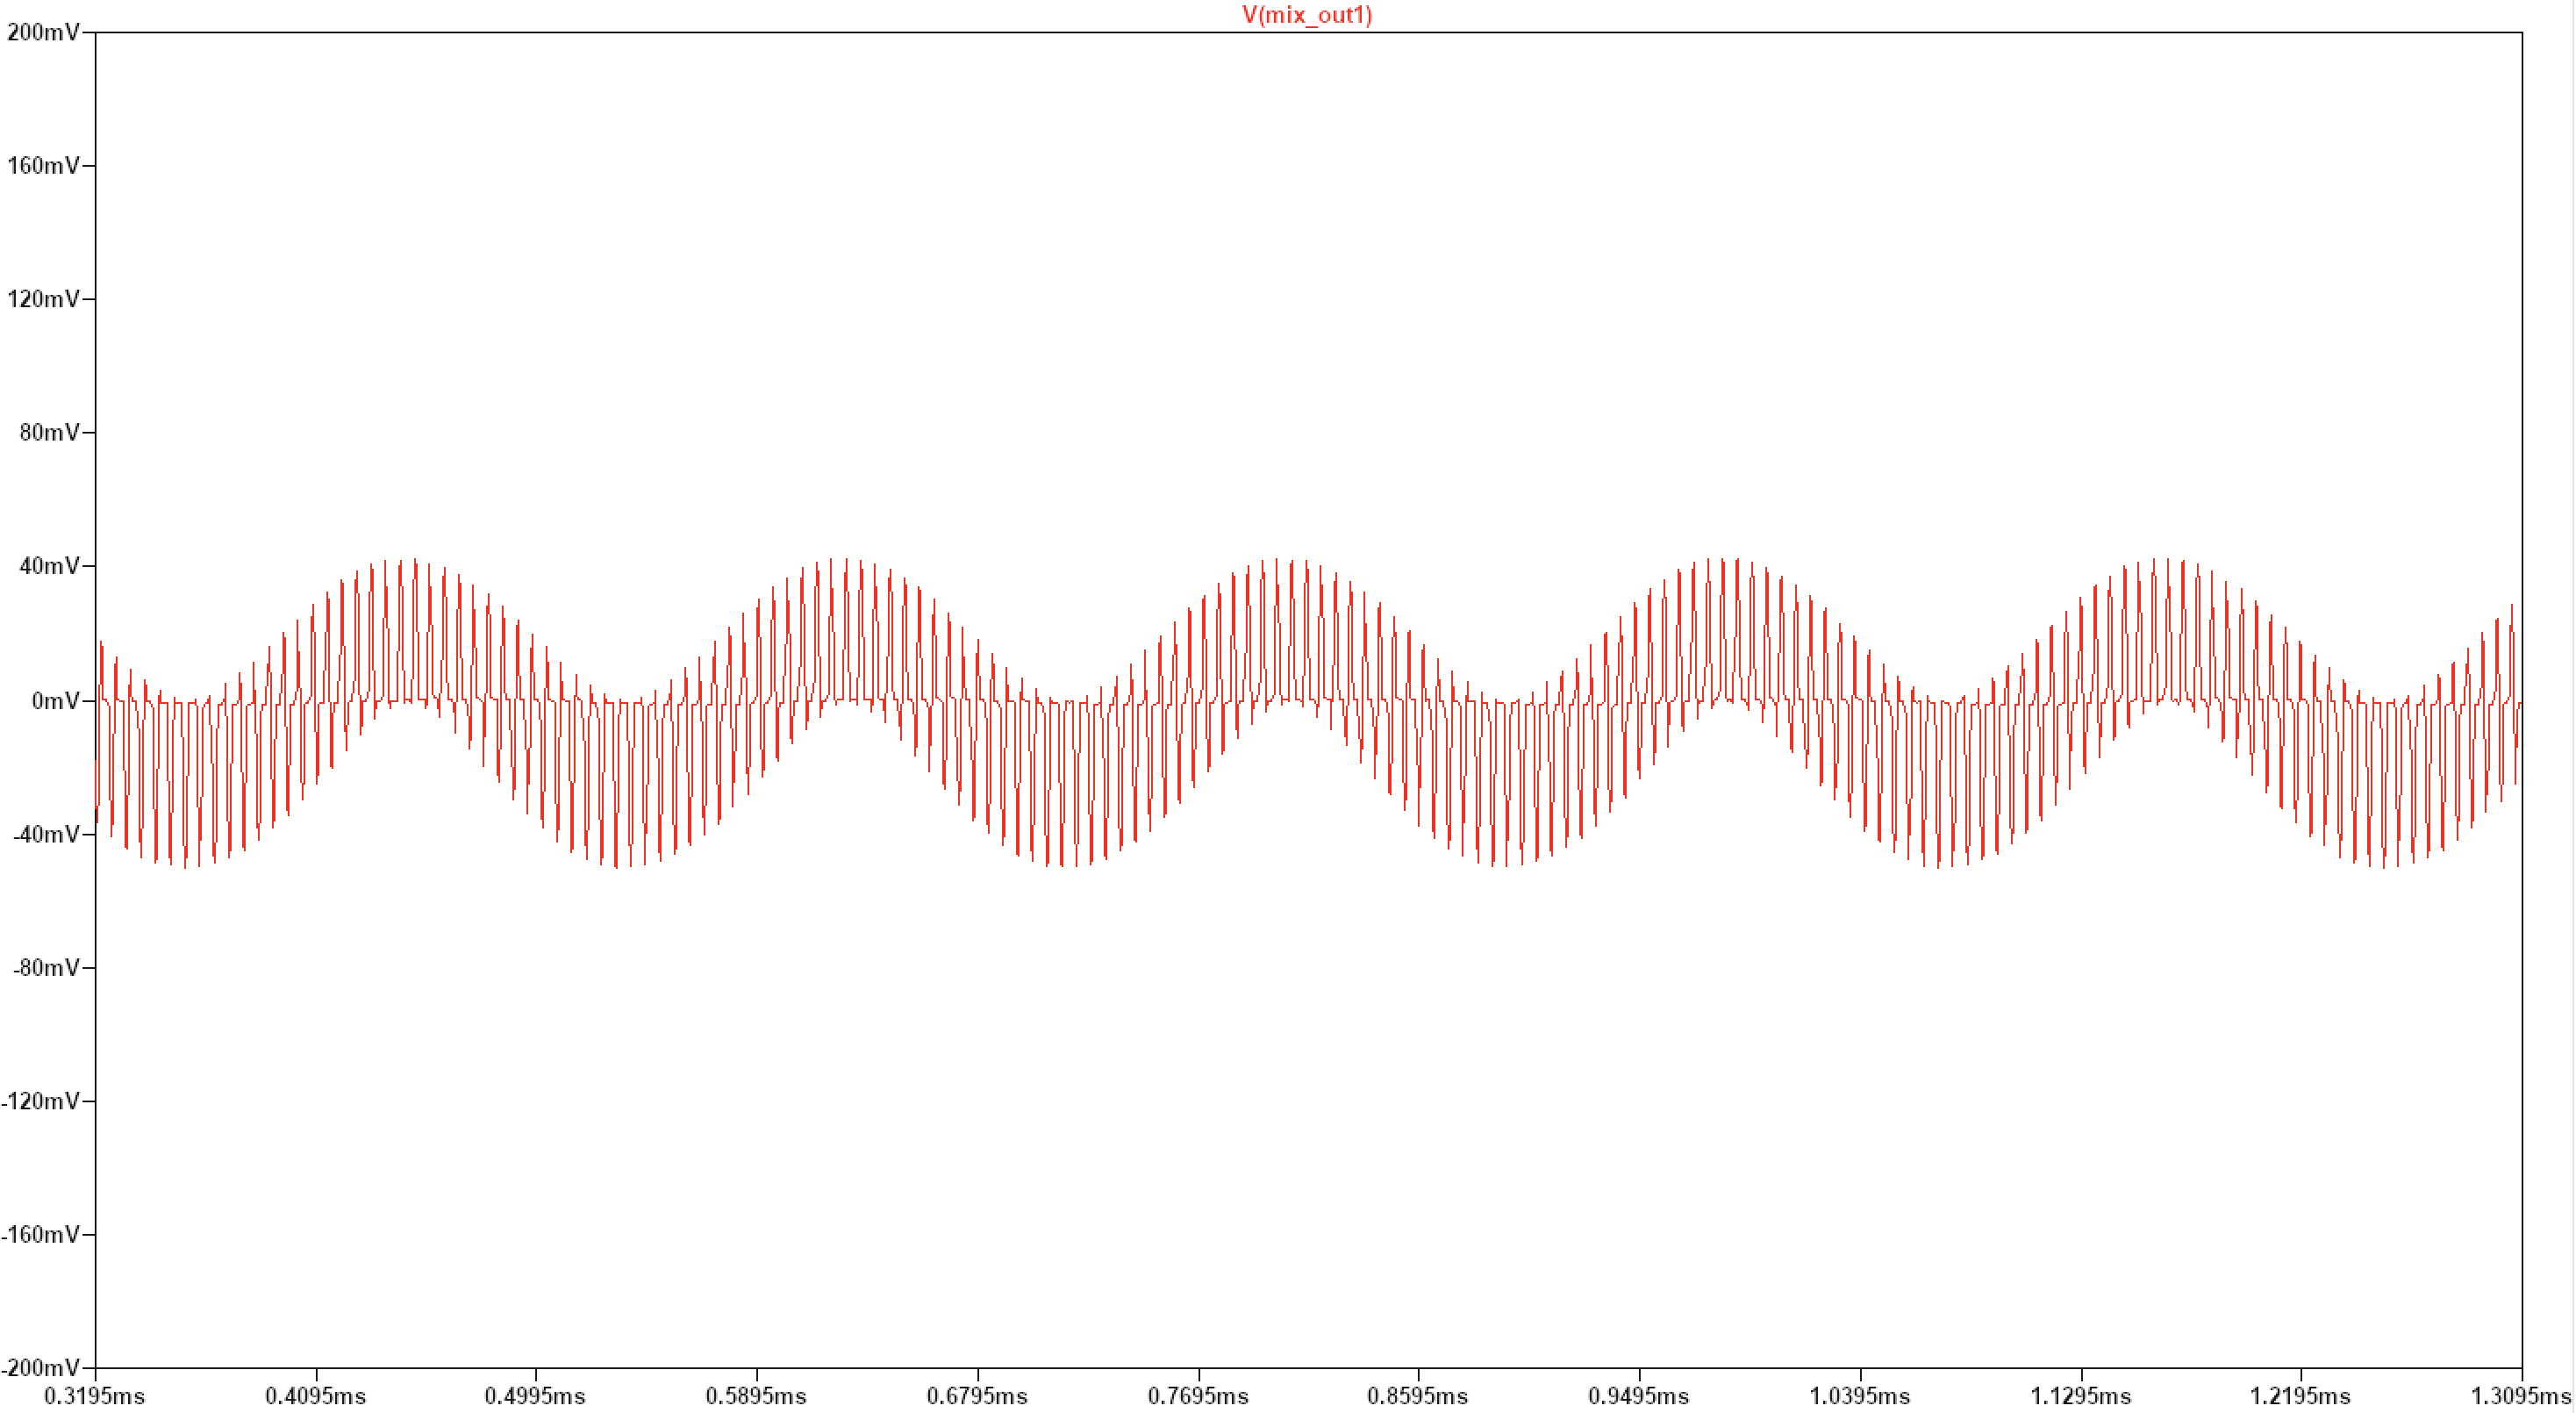
\includegraphics[width=\columnwidth]{images/165k-t.png}
        \caption{$f_{IN} = 165\text{ kHz}$ Transient}
    \end{subfigure}
    
    \vspace{0.3cm}
    \begin{subfigure}[b]{\columnwidth}
        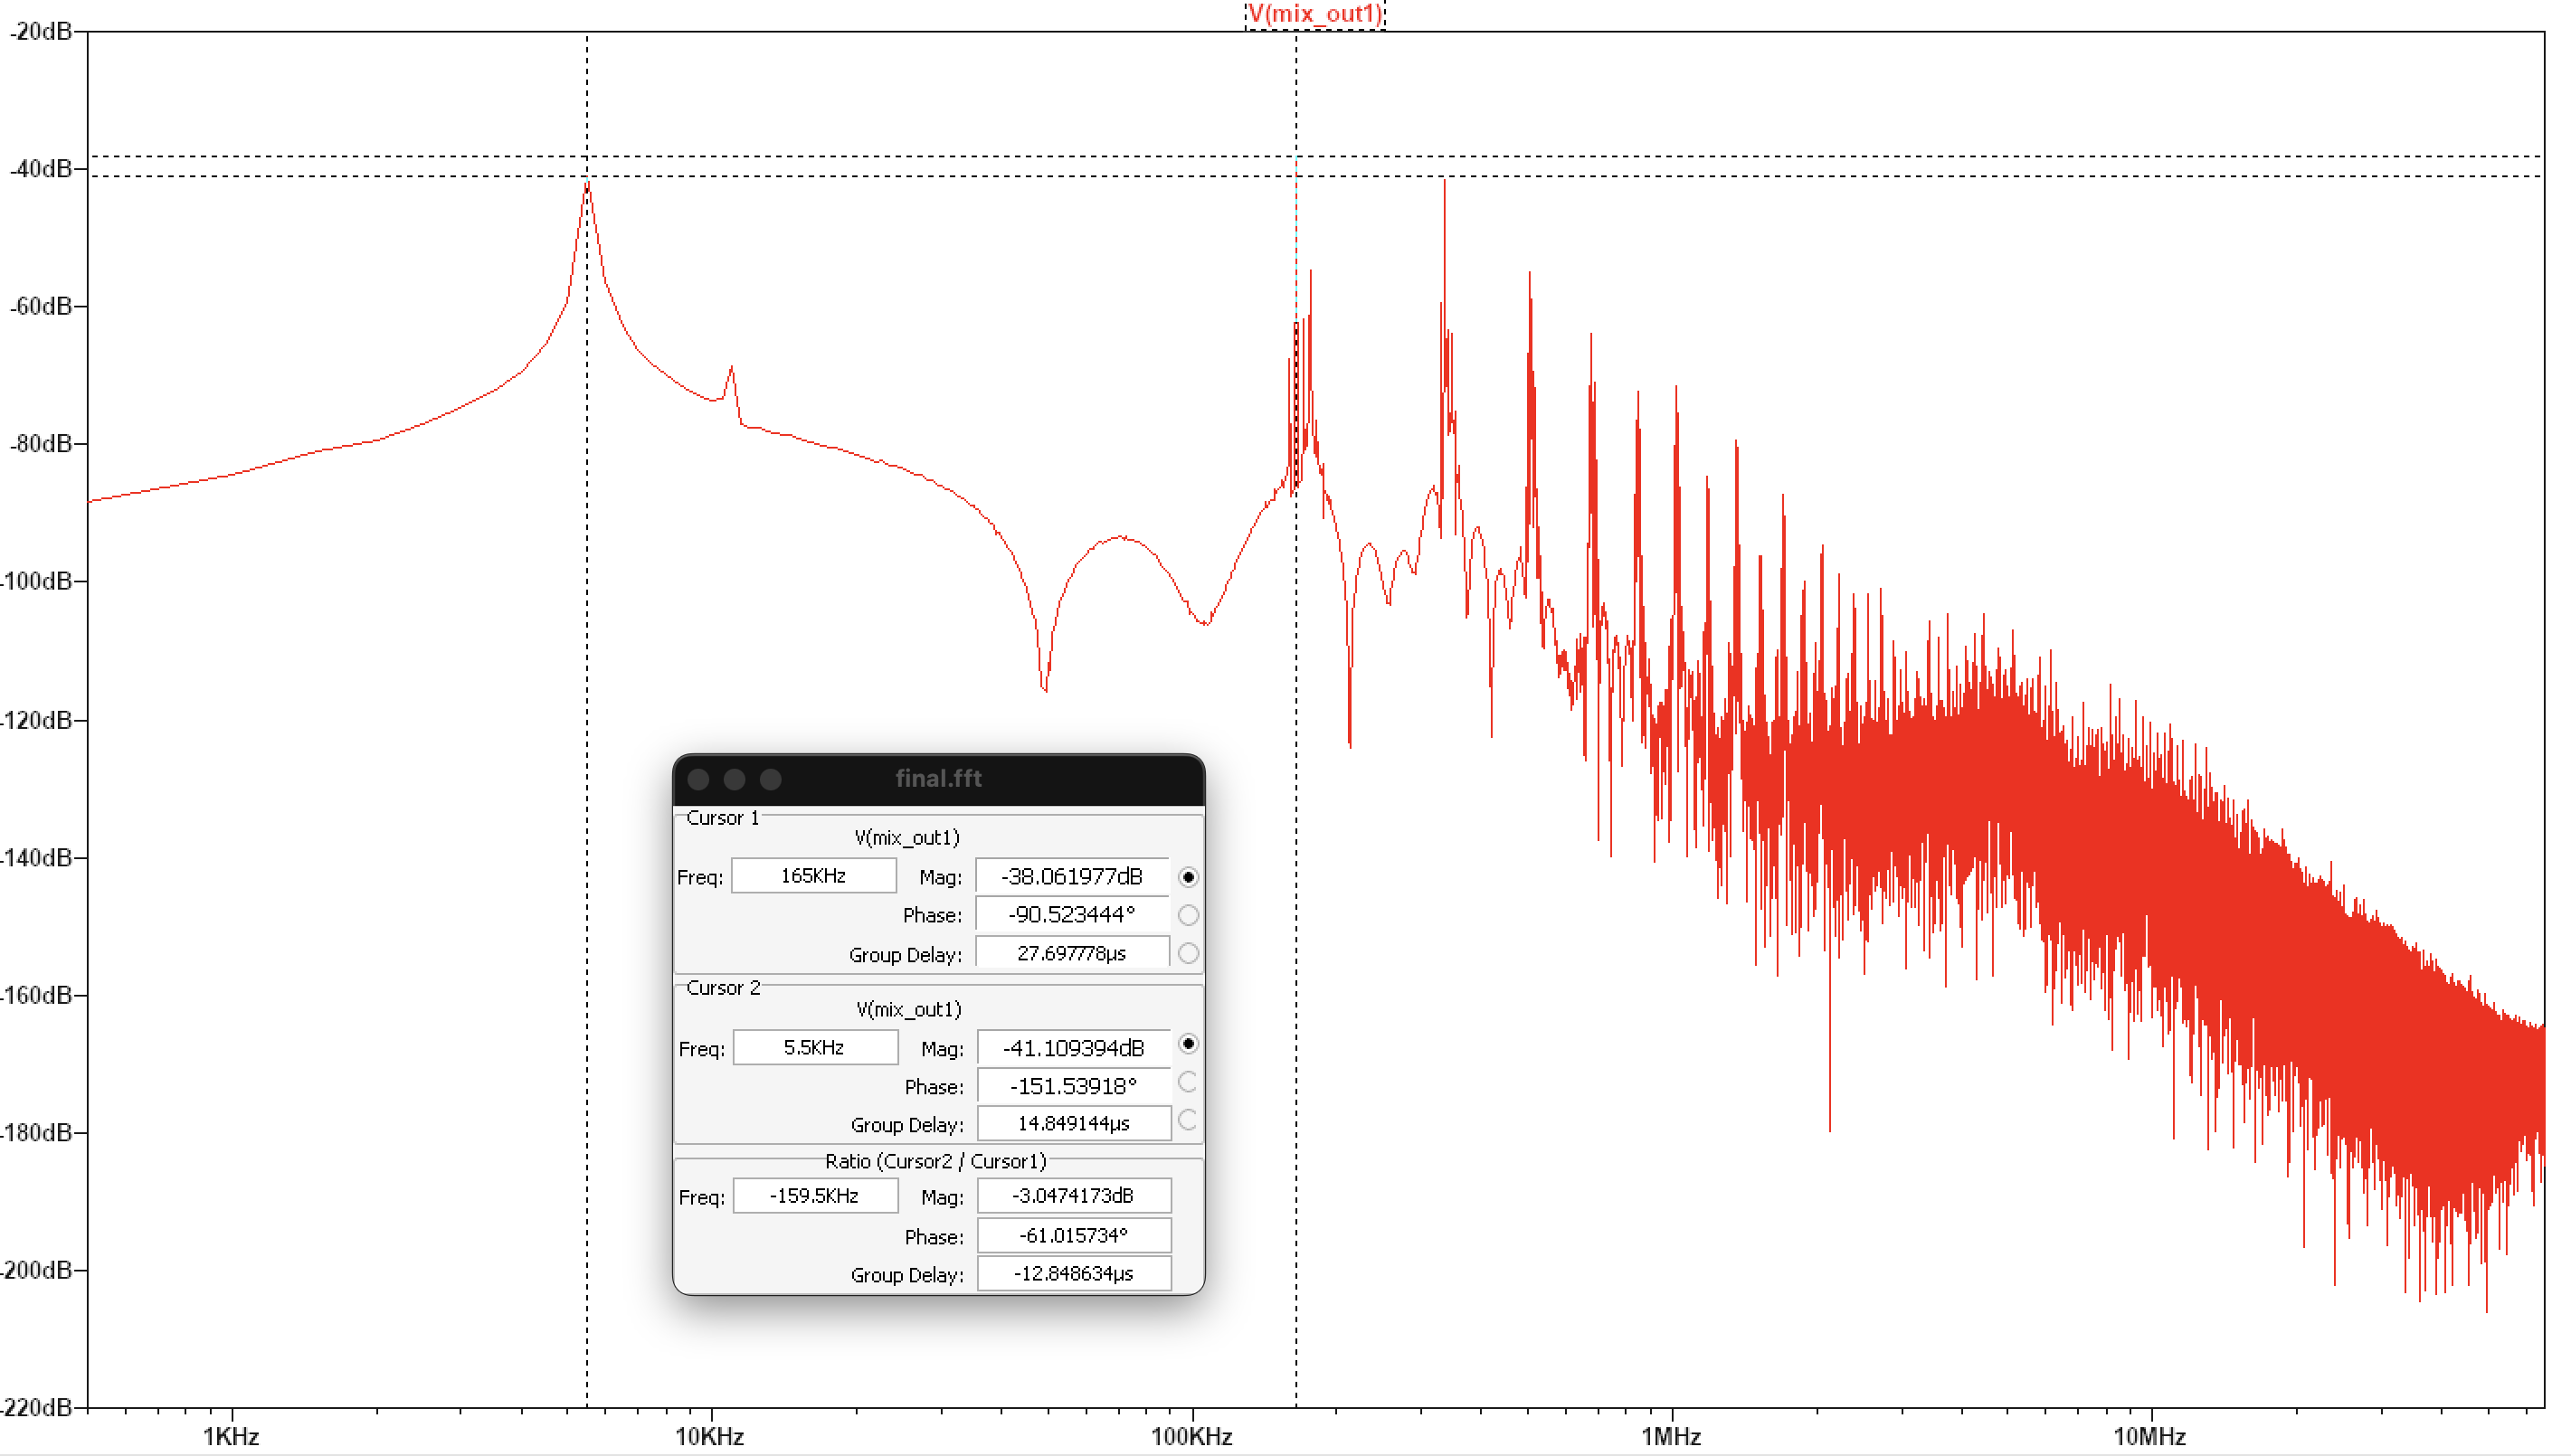
\includegraphics[width=\columnwidth]{images/165k-fft.png}
        \caption{$f_{IN} = 165\text{ kHz}$ FFT ($f_{IF} = 5\text{ kHz}$)}
    \end{subfigure}
    \caption{Mixer Output for $f_{IN} = 165\text{ kHz}$}
\end{figure}

\begin{figure}[htbp]
    \centering
    \begin{subfigure}[b]{\columnwidth}
        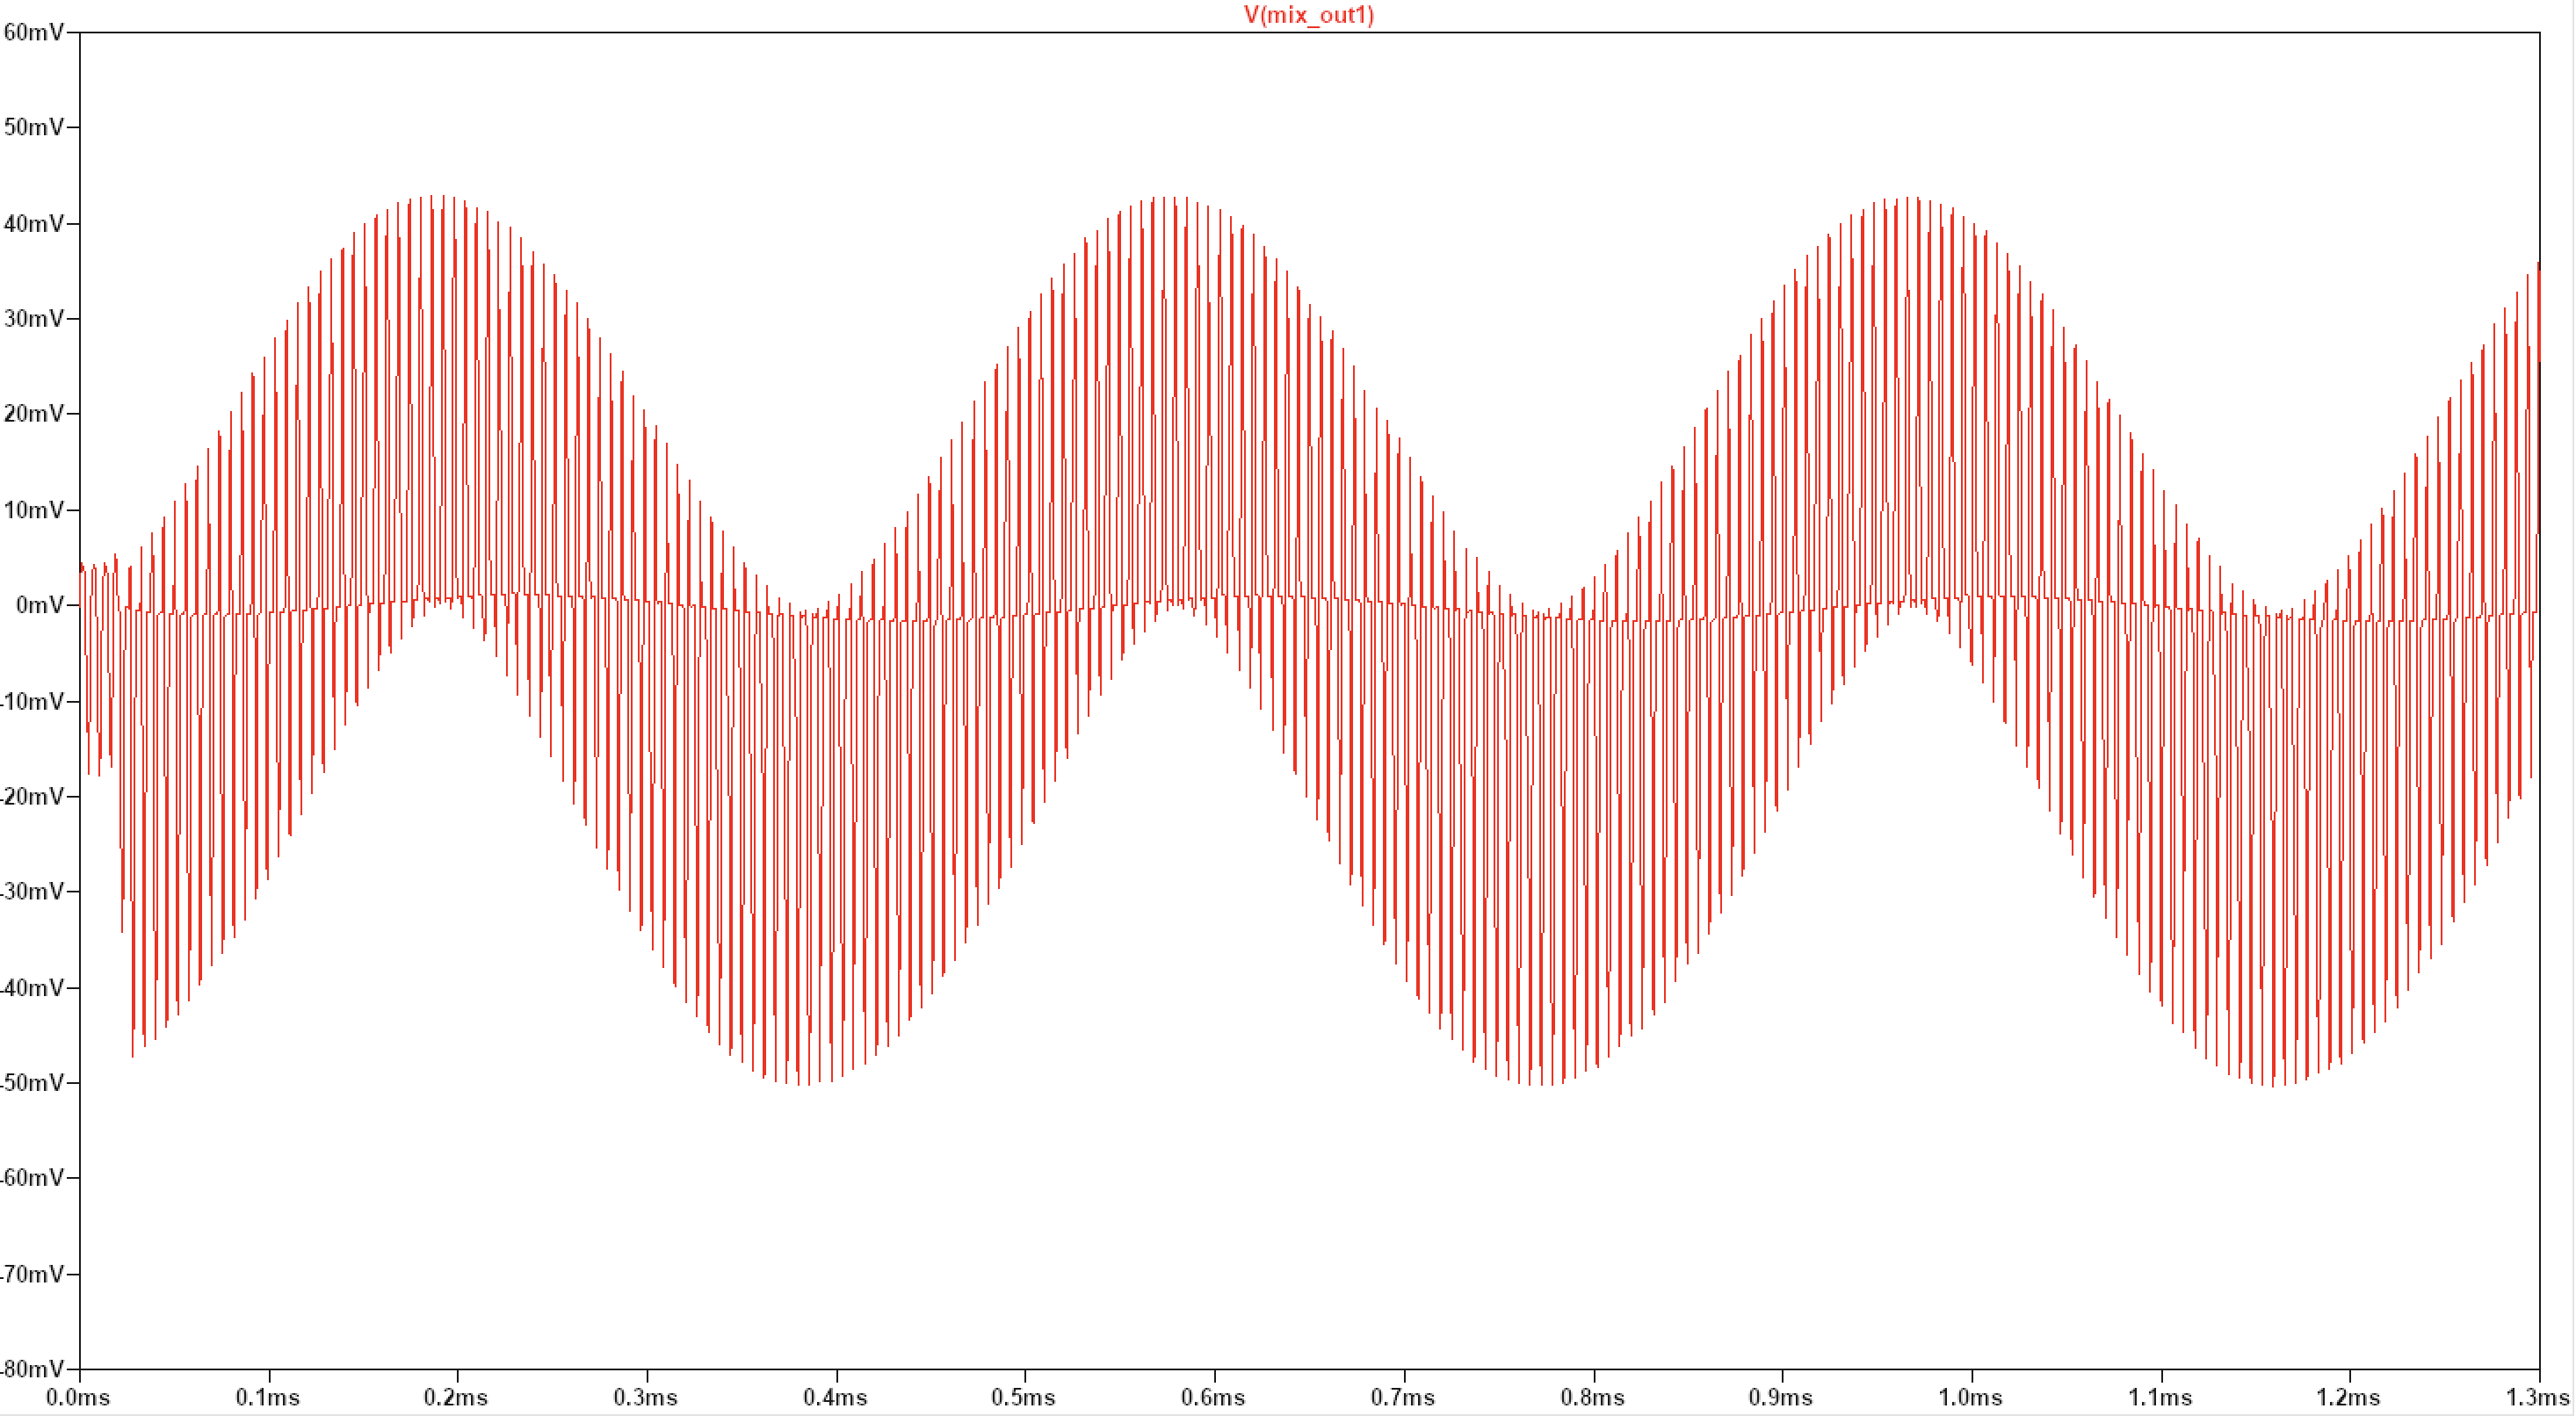
\includegraphics[width=\columnwidth]{images/168k-t.png}
        \caption{$f_{IN} = 168\text{ kHz}$ Transient}
    \end{subfigure}
    
    \vspace{0.3cm}
    \begin{subfigure}[b]{\columnwidth}
        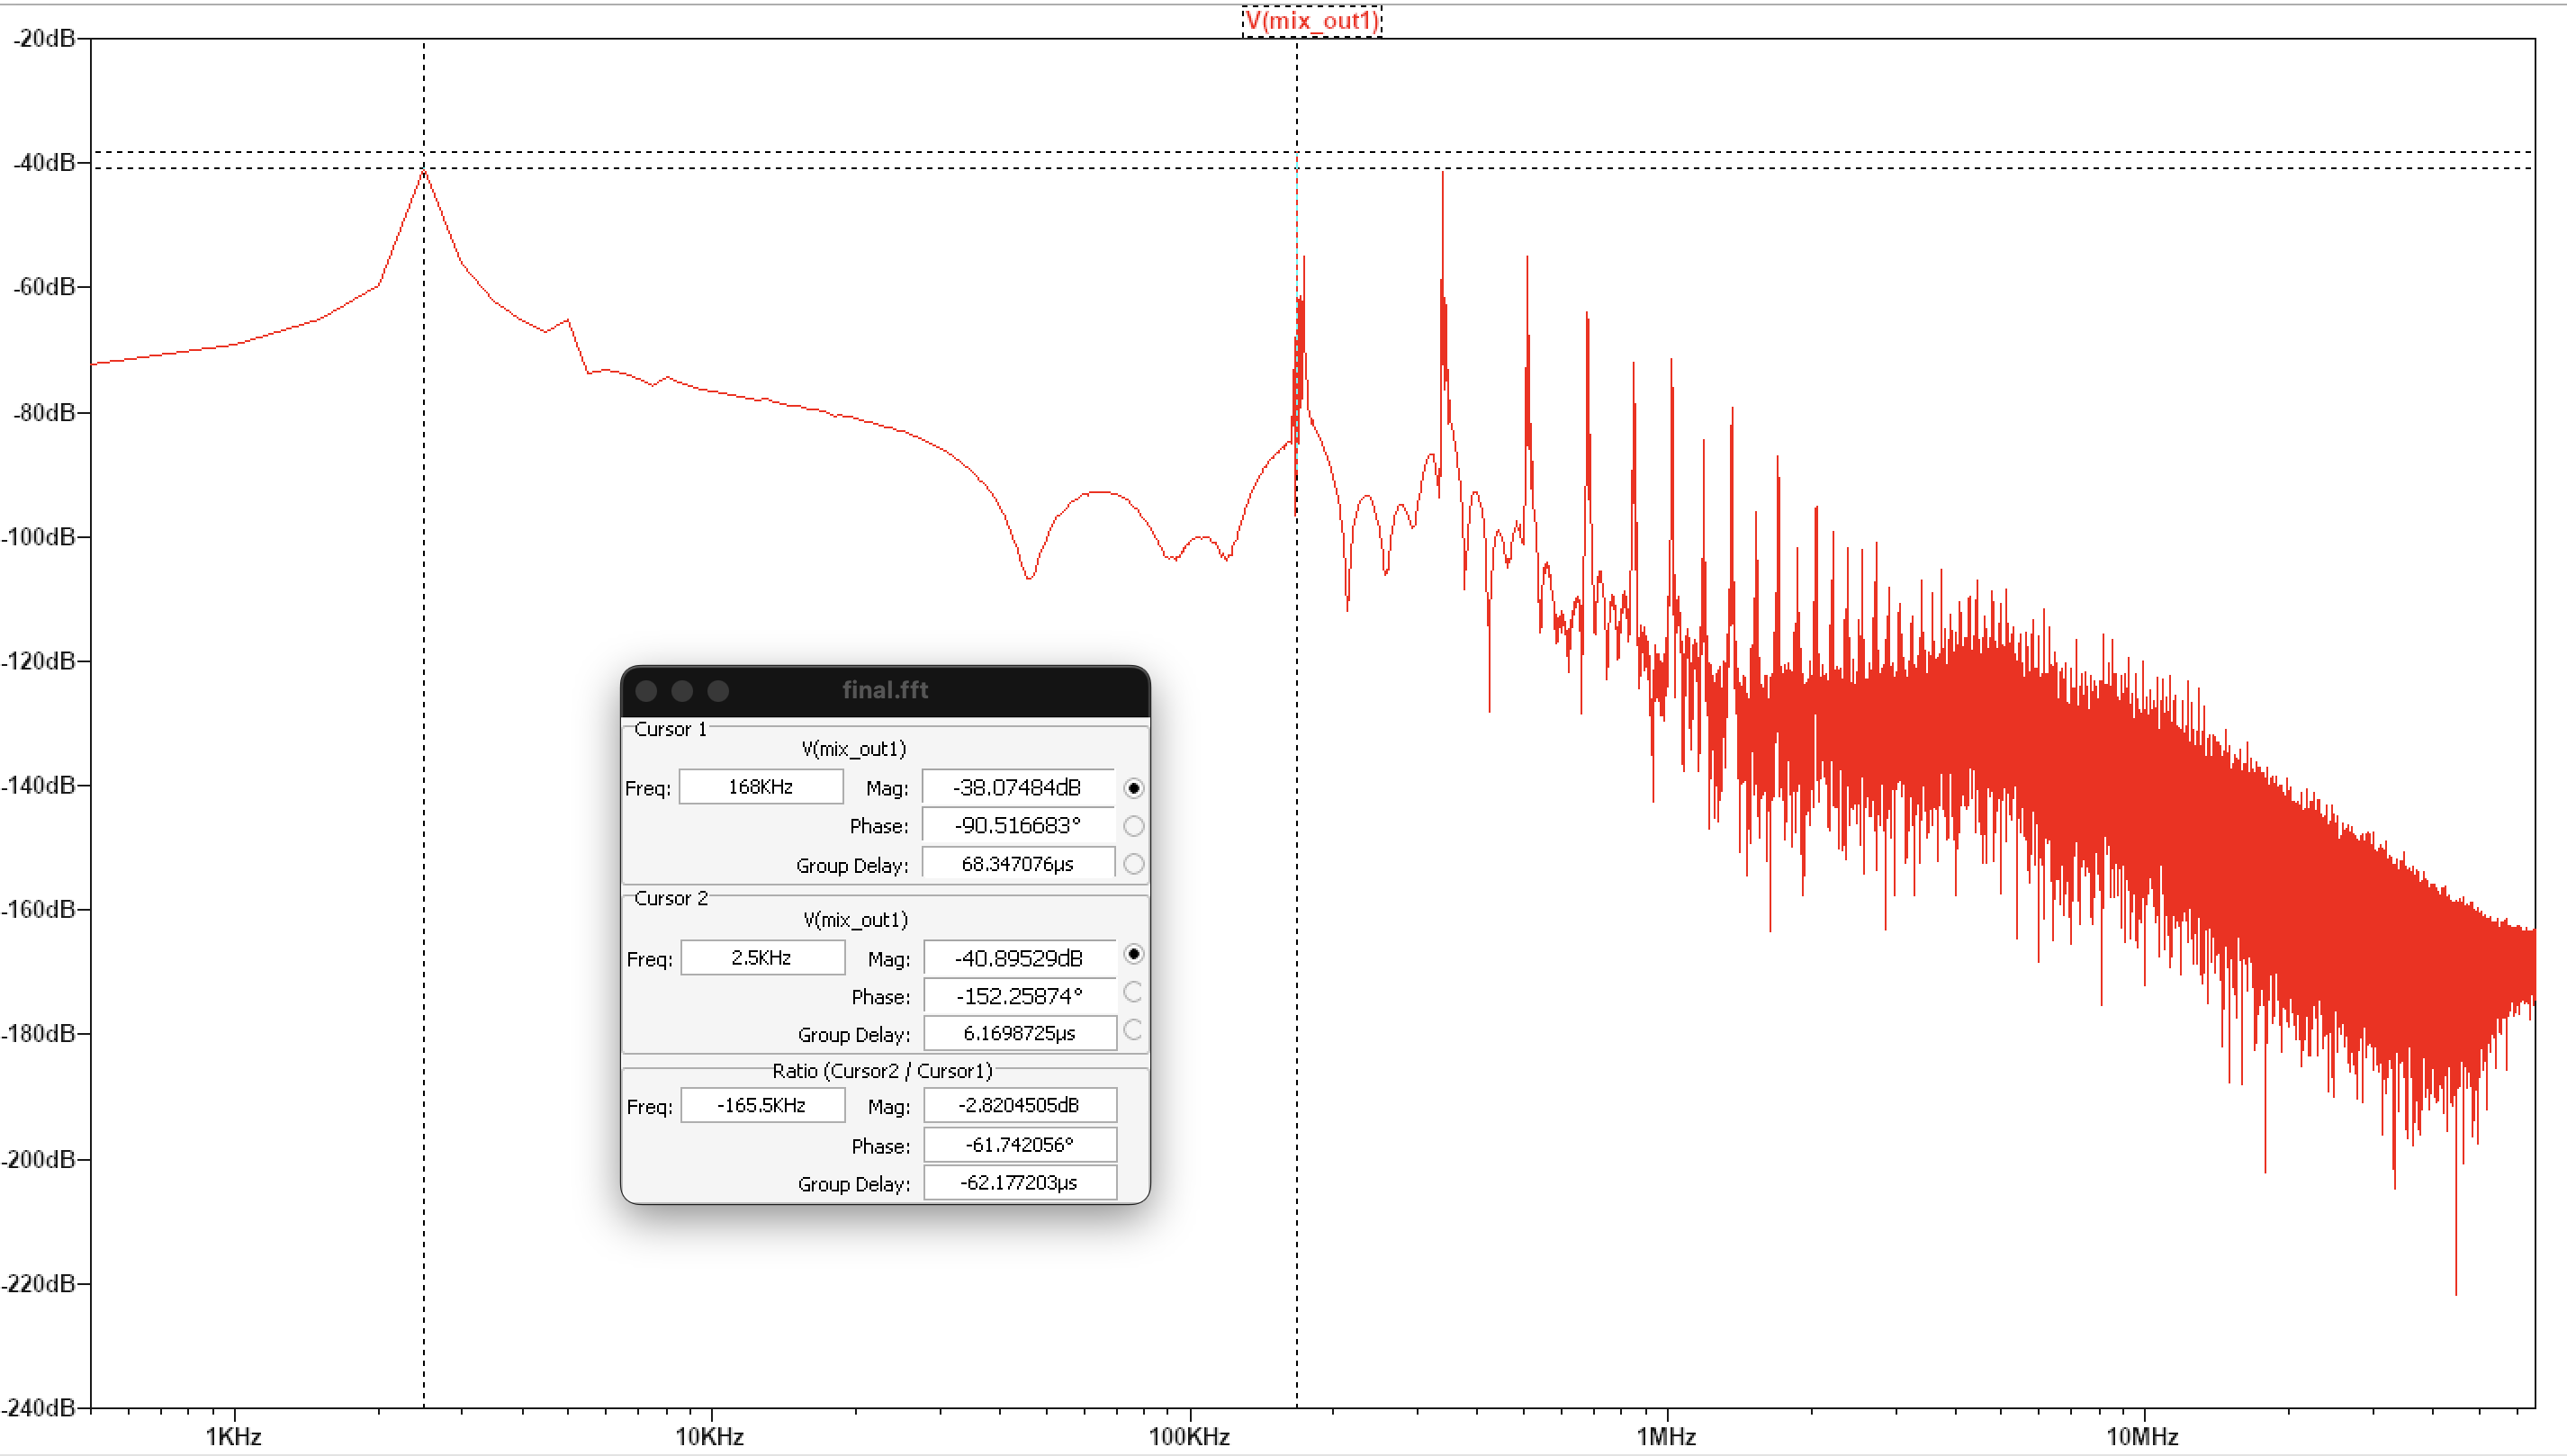
\includegraphics[width=\columnwidth]{images/168k-fft.png}
        \caption{$f_{IN} = 168\text{ kHz}$ FFT ($f_{IF} = 2\text{ kHz}$)}
    \end{subfigure}
    \caption{Mixer Output for $f_{IN} = 168\text{ kHz}$}
\end{figure}

\begin{figure}[htbp]
    \centering
    \begin{subfigure}[b]{\columnwidth}
        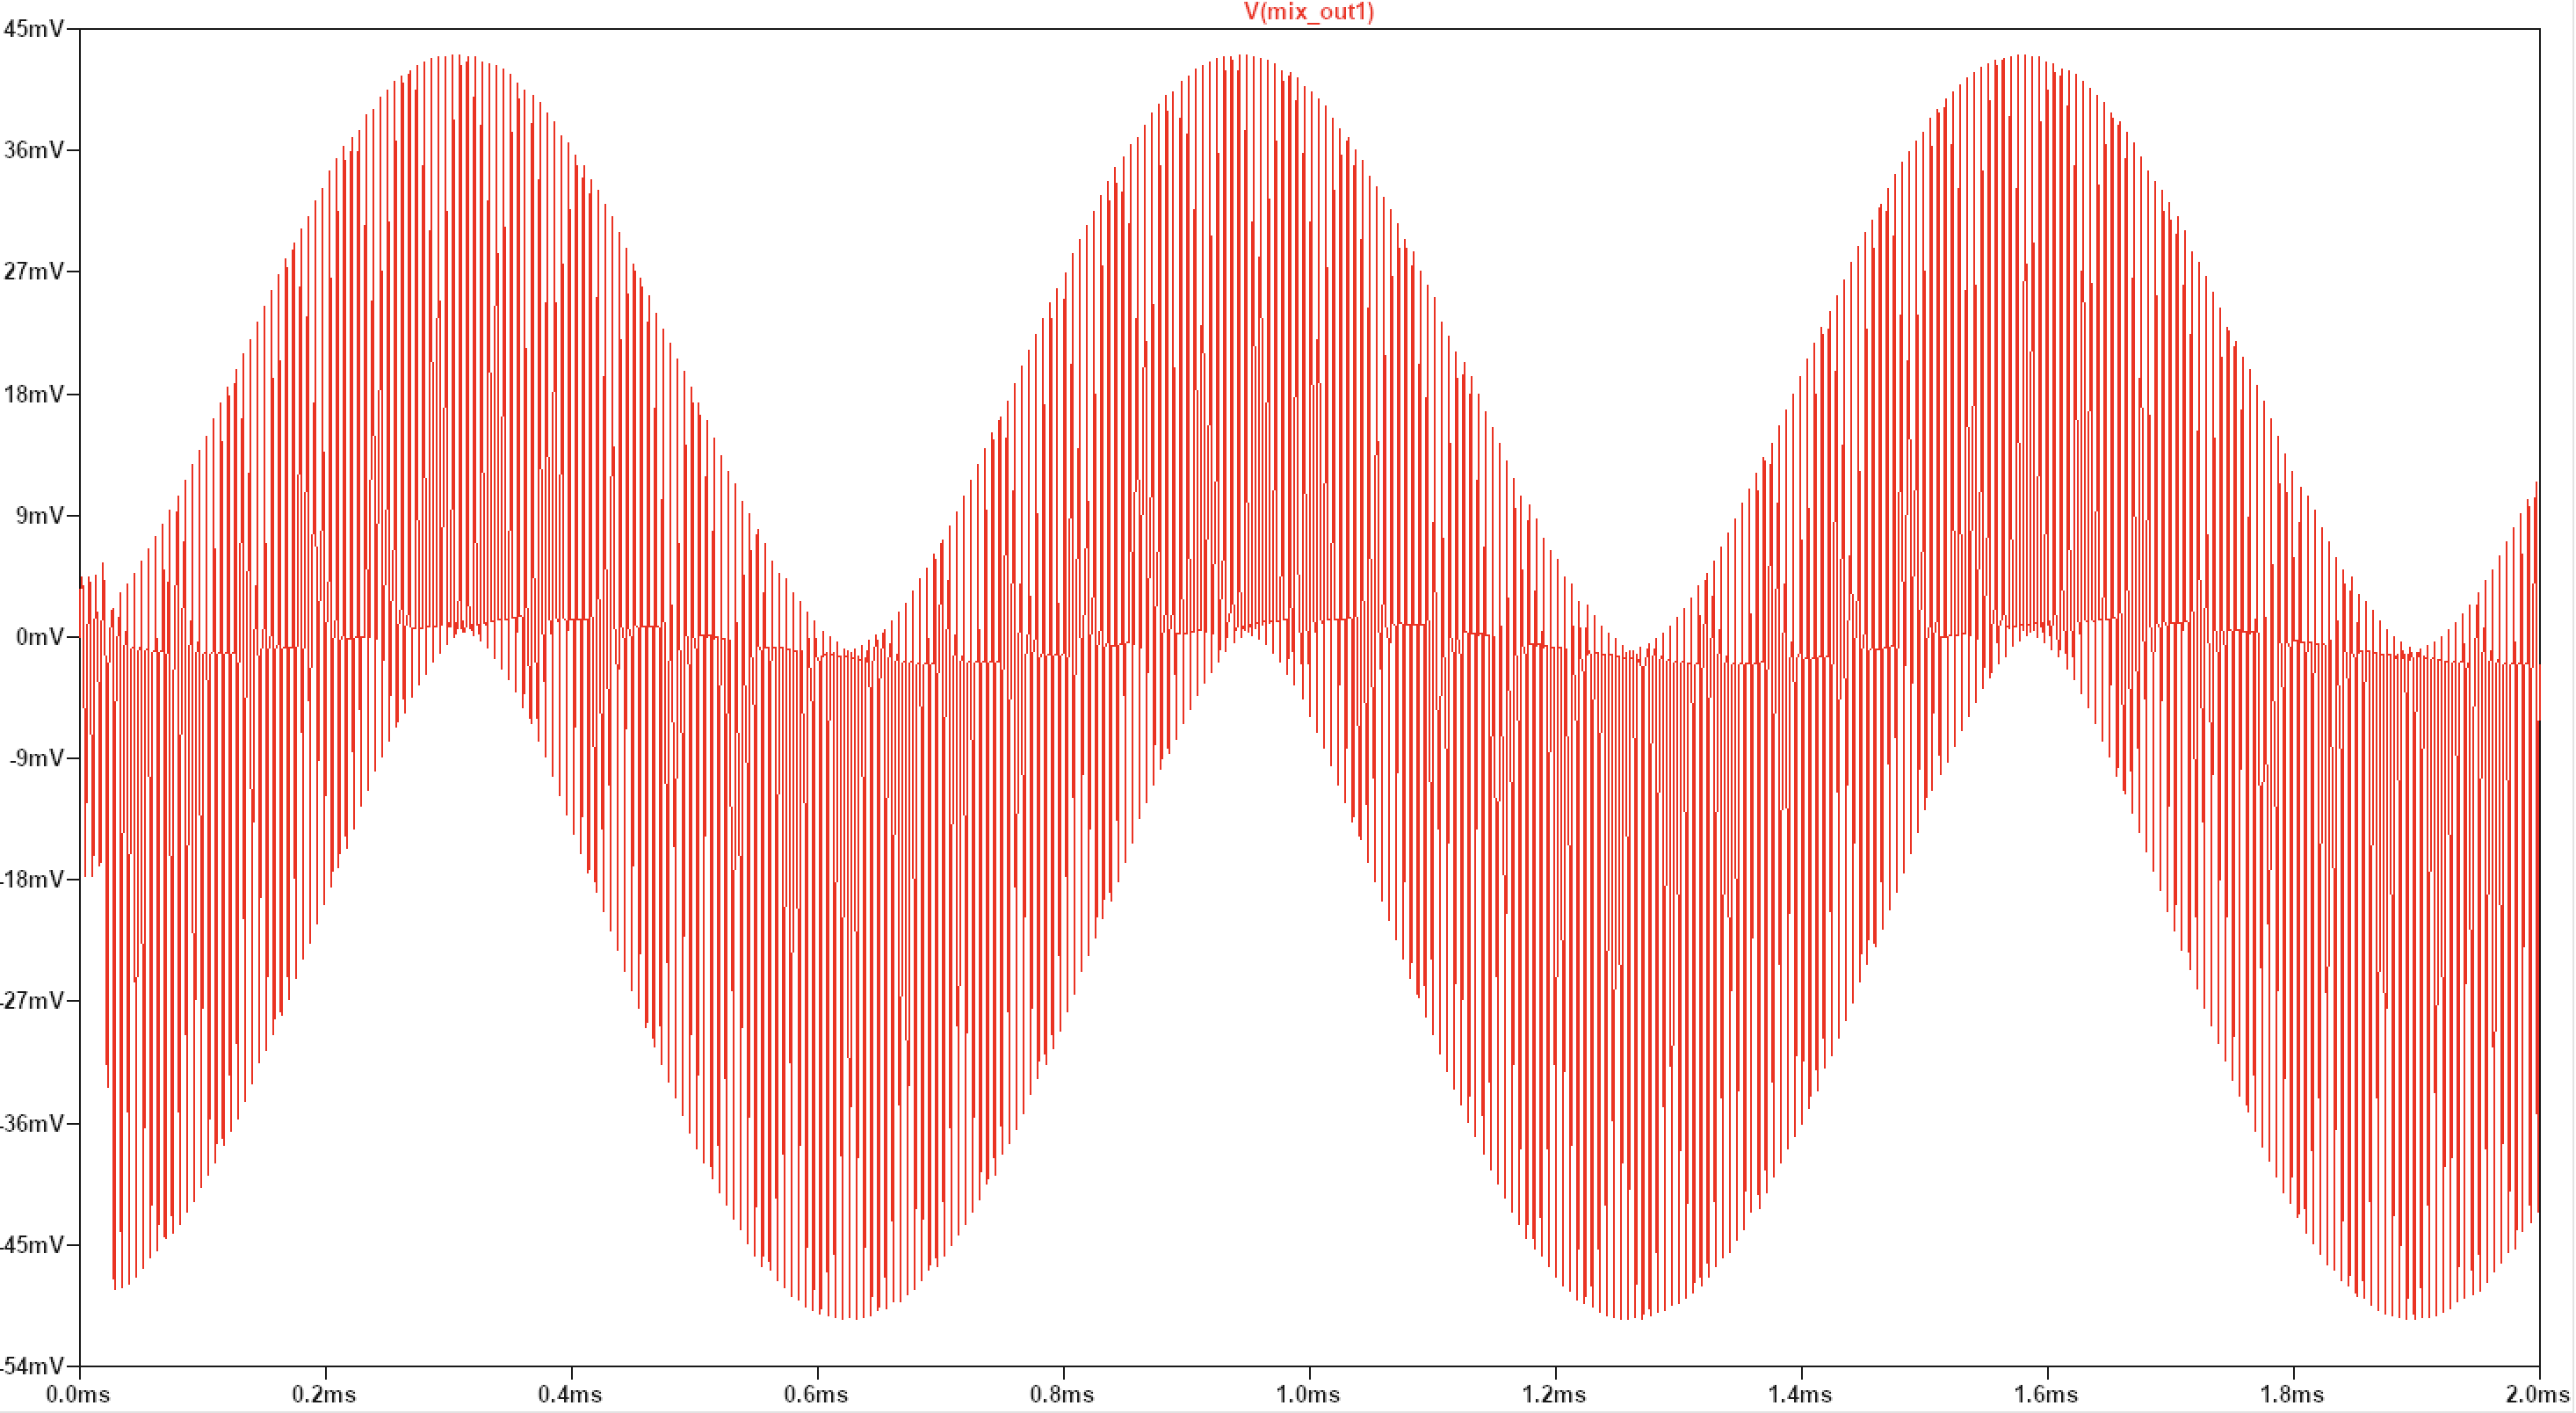
\includegraphics[width=\columnwidth]{images/169k-t.png}
        \caption{$f_{IN} = 169\text{ kHz}$ Transient}
    \end{subfigure}
    
    \vspace{0.3cm}
    \begin{subfigure}[b]{\columnwidth}
        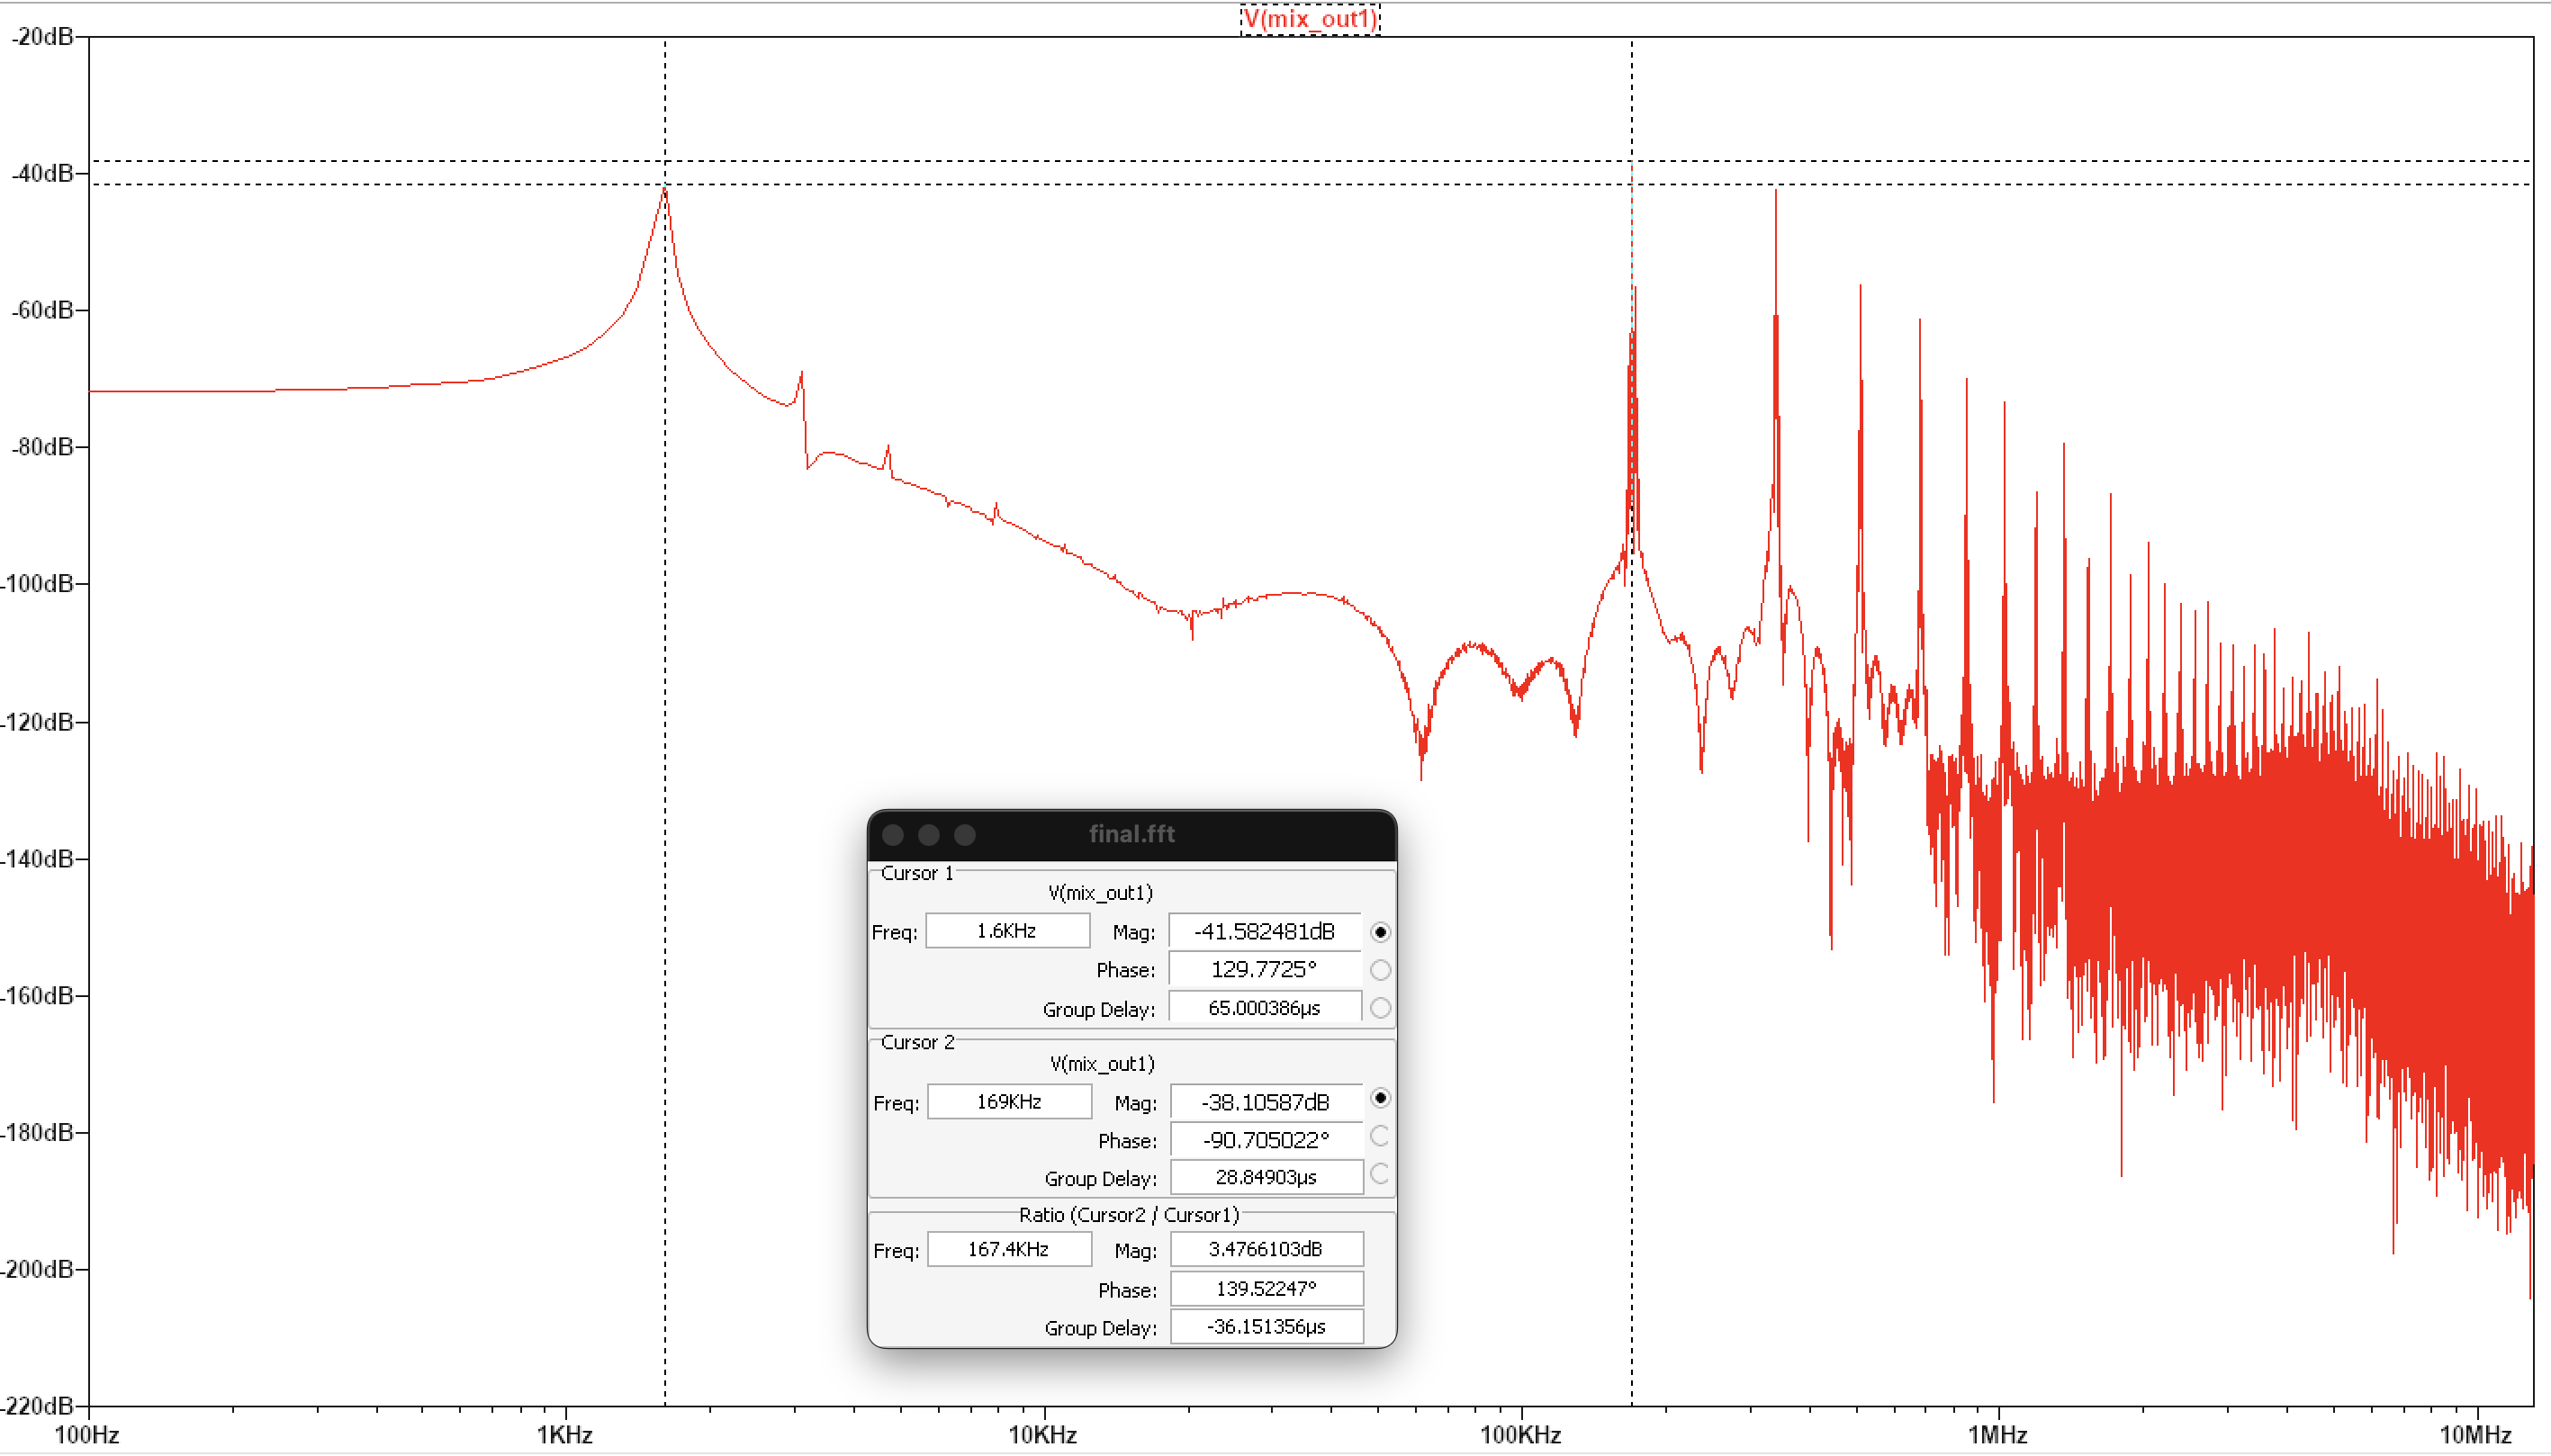
\includegraphics[width=\columnwidth]{images/169k-fft.png}
        \caption{$f_{IN} = 169\text{ kHz}$ FFT ($f_{IF} = 1\text{ kHz}$)}
    \end{subfigure}
    \caption{Mixer Output for $f_{IN} = 169\text{ kHz}$}
    \label{fig:mixer_sweep_below}
\end{figure}

\begin{figure}[htbp]
    \centering
    \begin{subfigure}[b]{\columnwidth}
        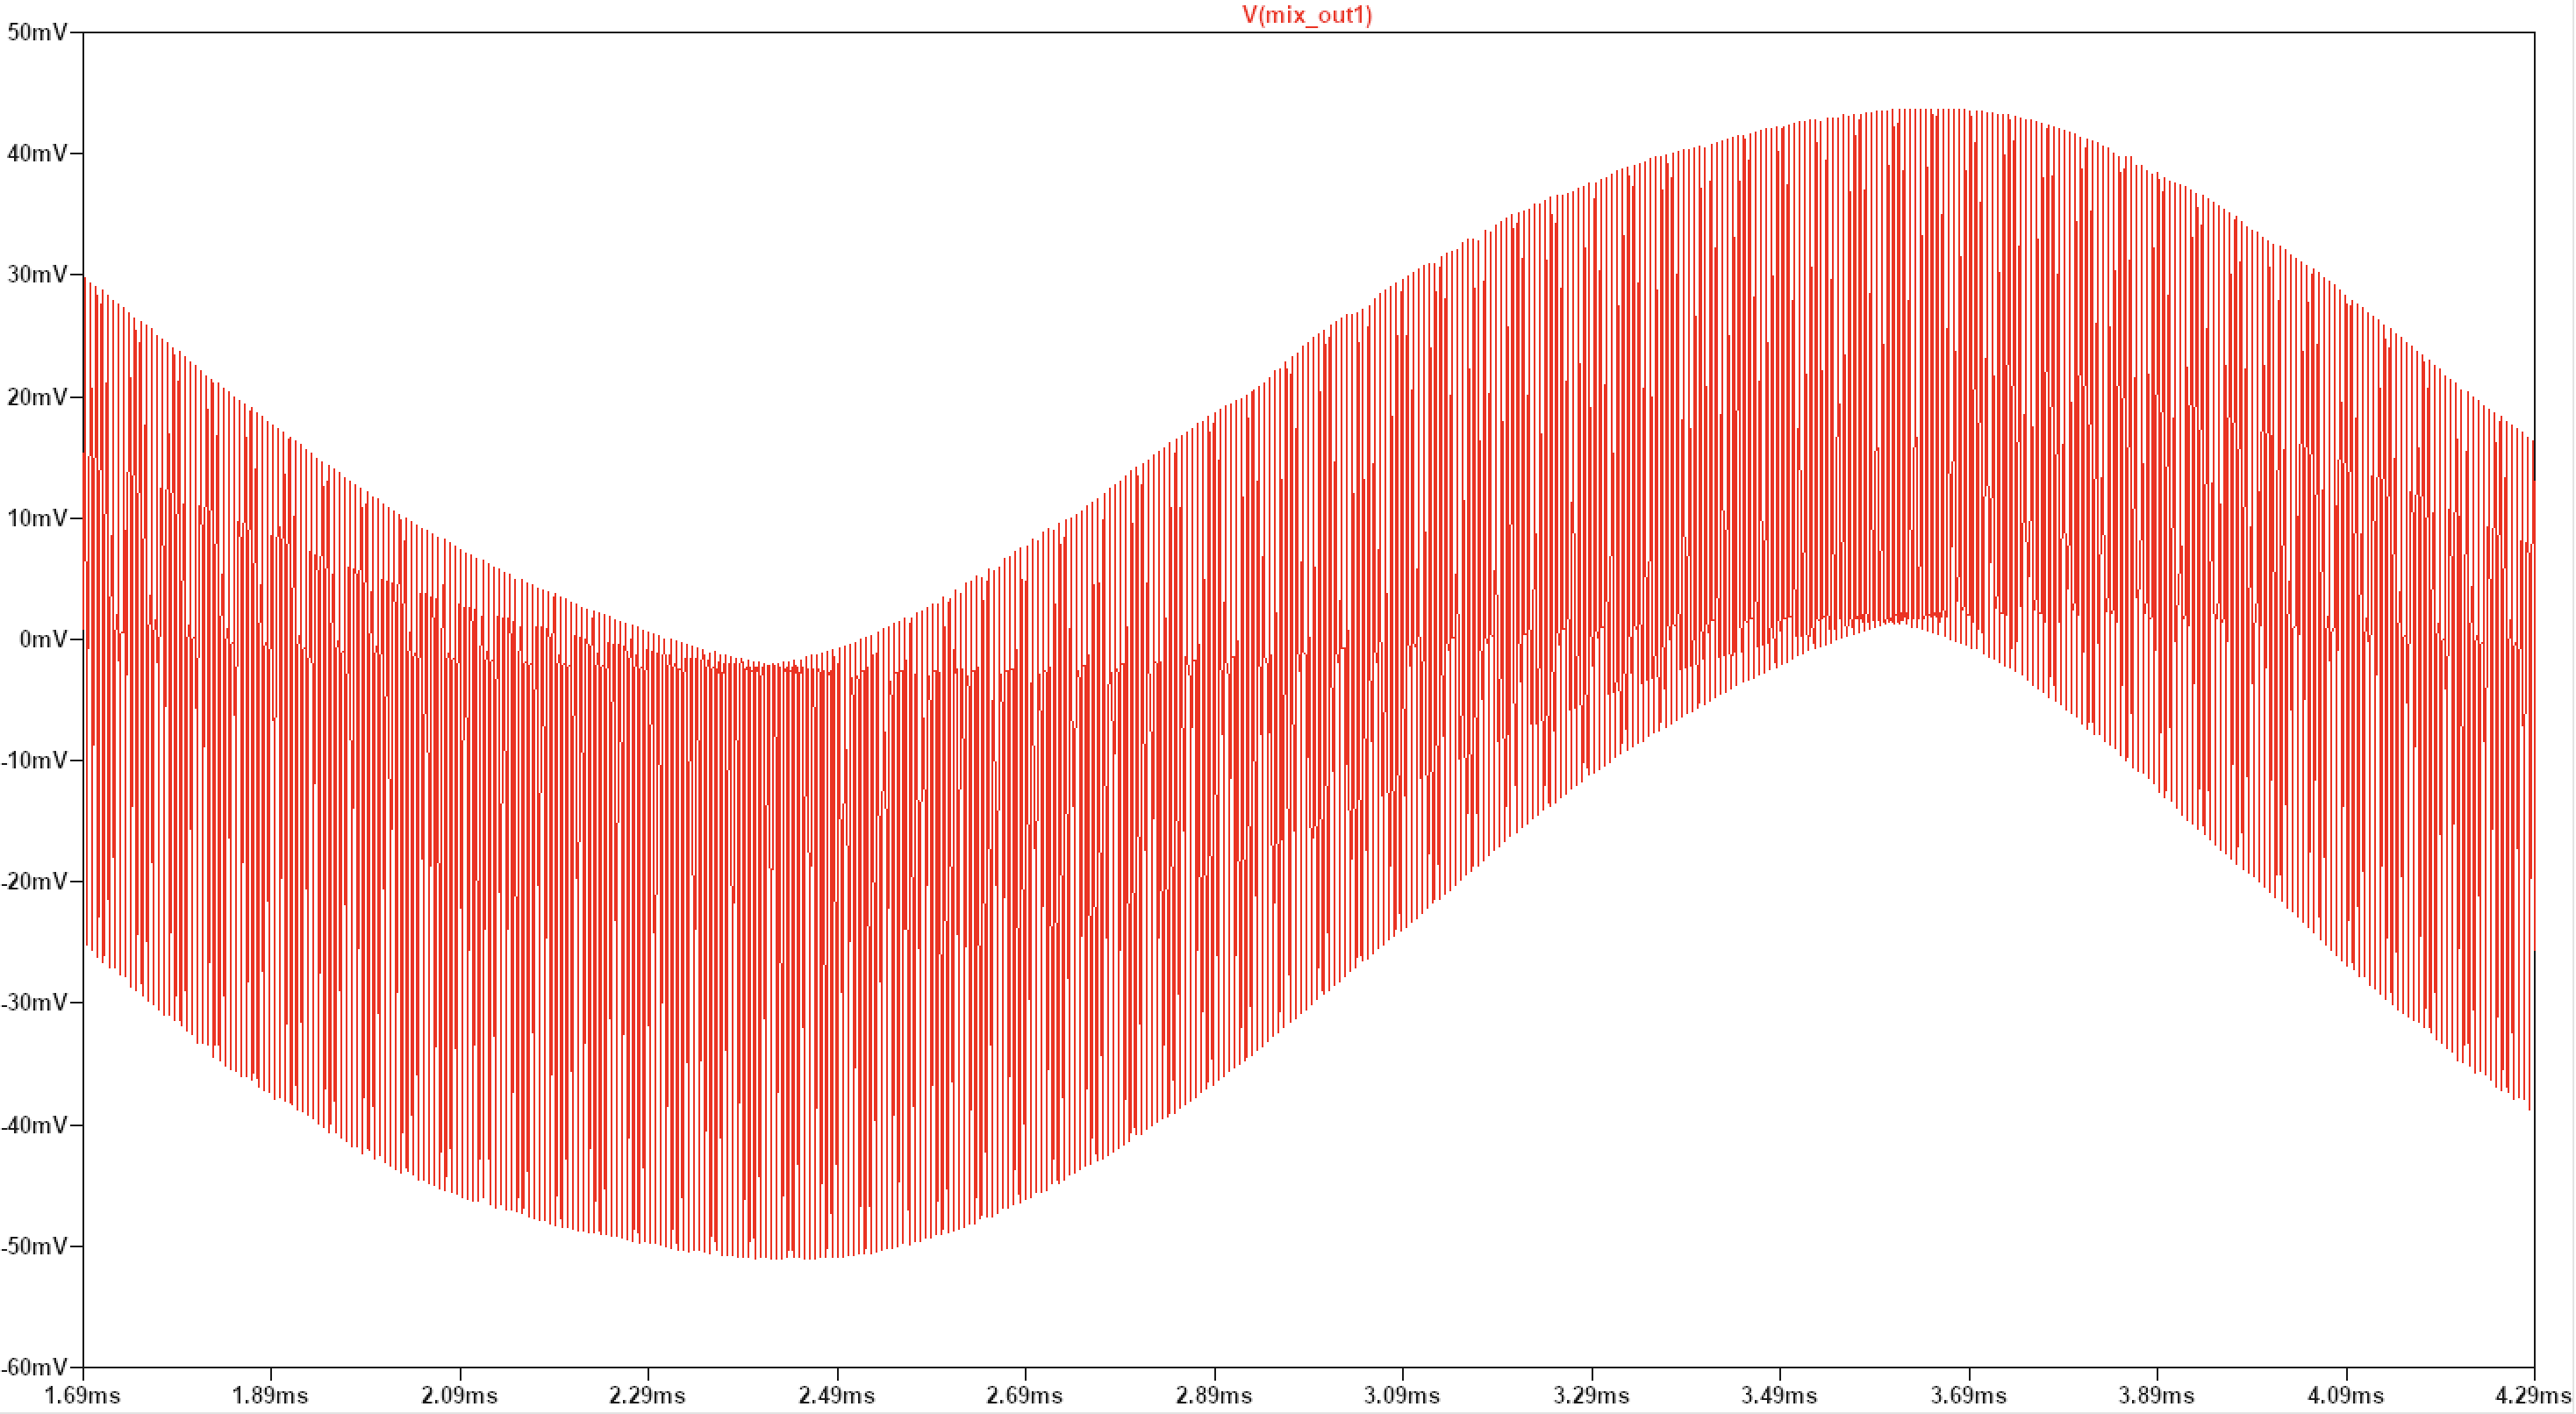
\includegraphics[width=\columnwidth]{images/171k-t.png}
        \caption{$f_{IN} = 171\text{ kHz}$ Transient}
    \end{subfigure}
    
    \vspace{0.3cm}
    \begin{subfigure}[b]{\columnwidth}
        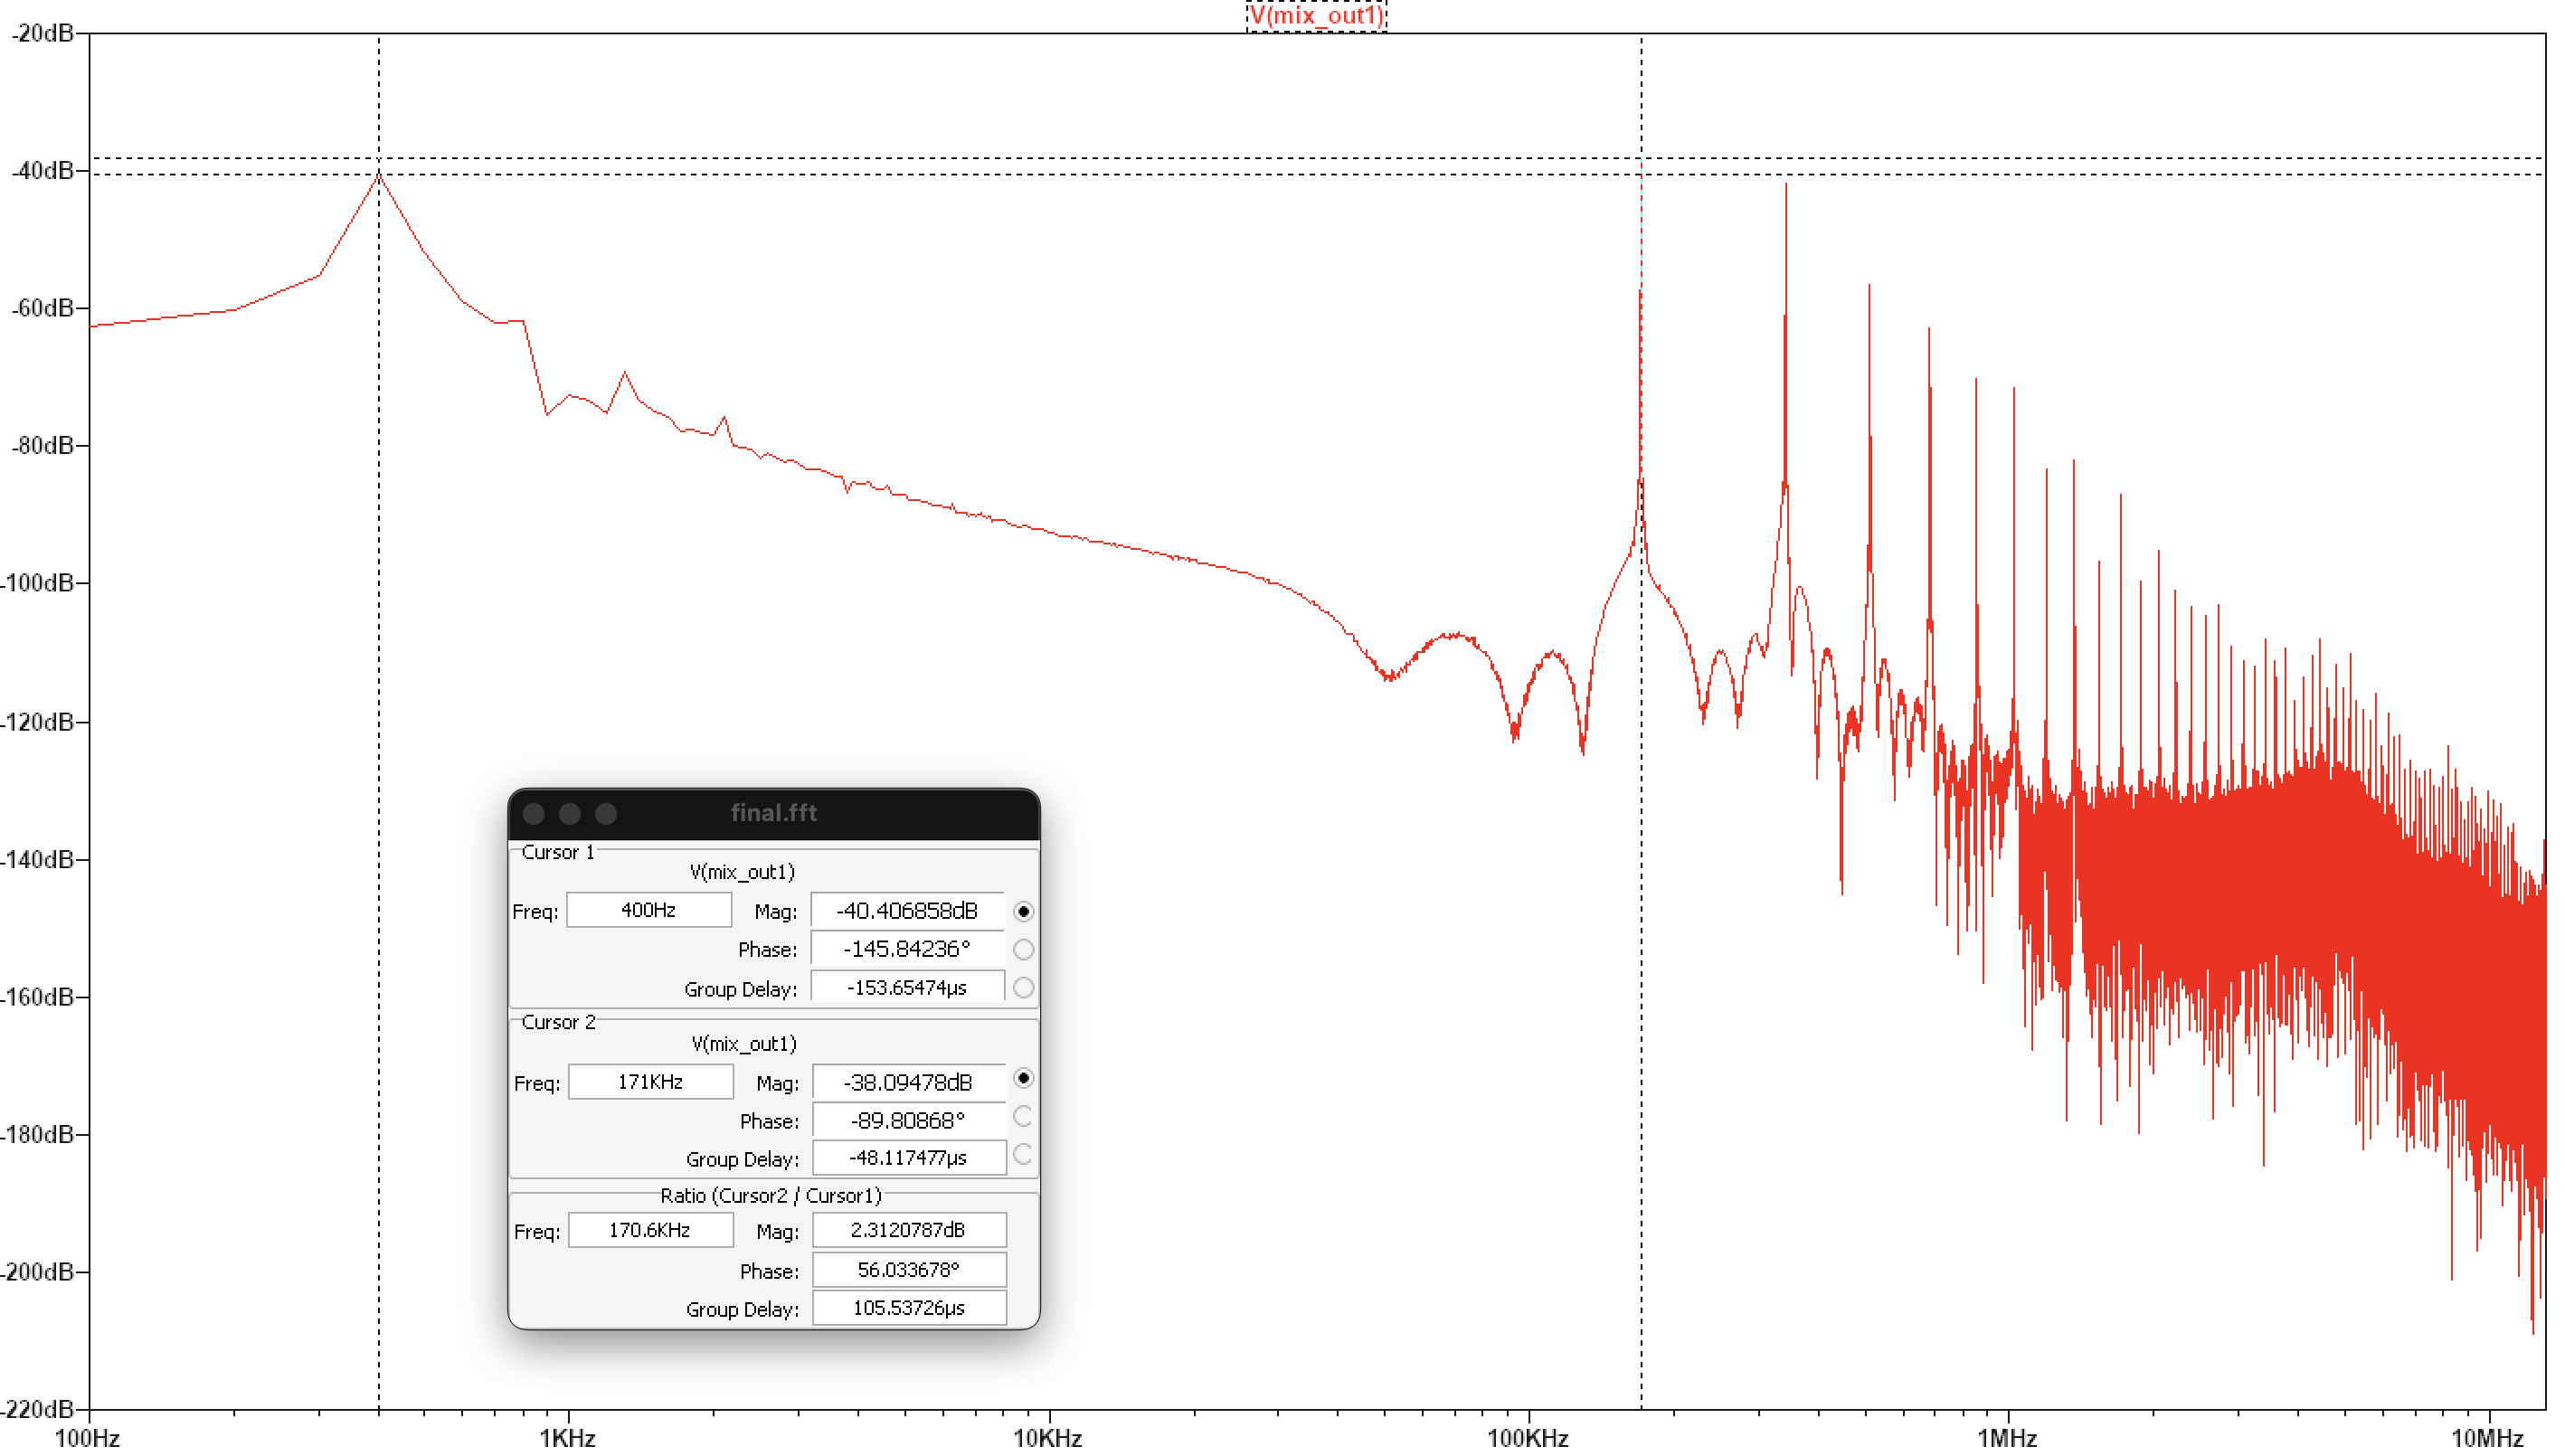
\includegraphics[width=\columnwidth]{images/171k-fft.png}
        \caption{$f_{IN} = 171\text{ kHz}$ FFT ($f_{IF} = 1\text{ kHz}$)}
    \end{subfigure}
    \caption{Mixer Output for $f_{IN} = 171\text{ kHz}$}
\end{figure}

\begin{figure}[htbp]
    \centering
    \begin{subfigure}[b]{\columnwidth}
        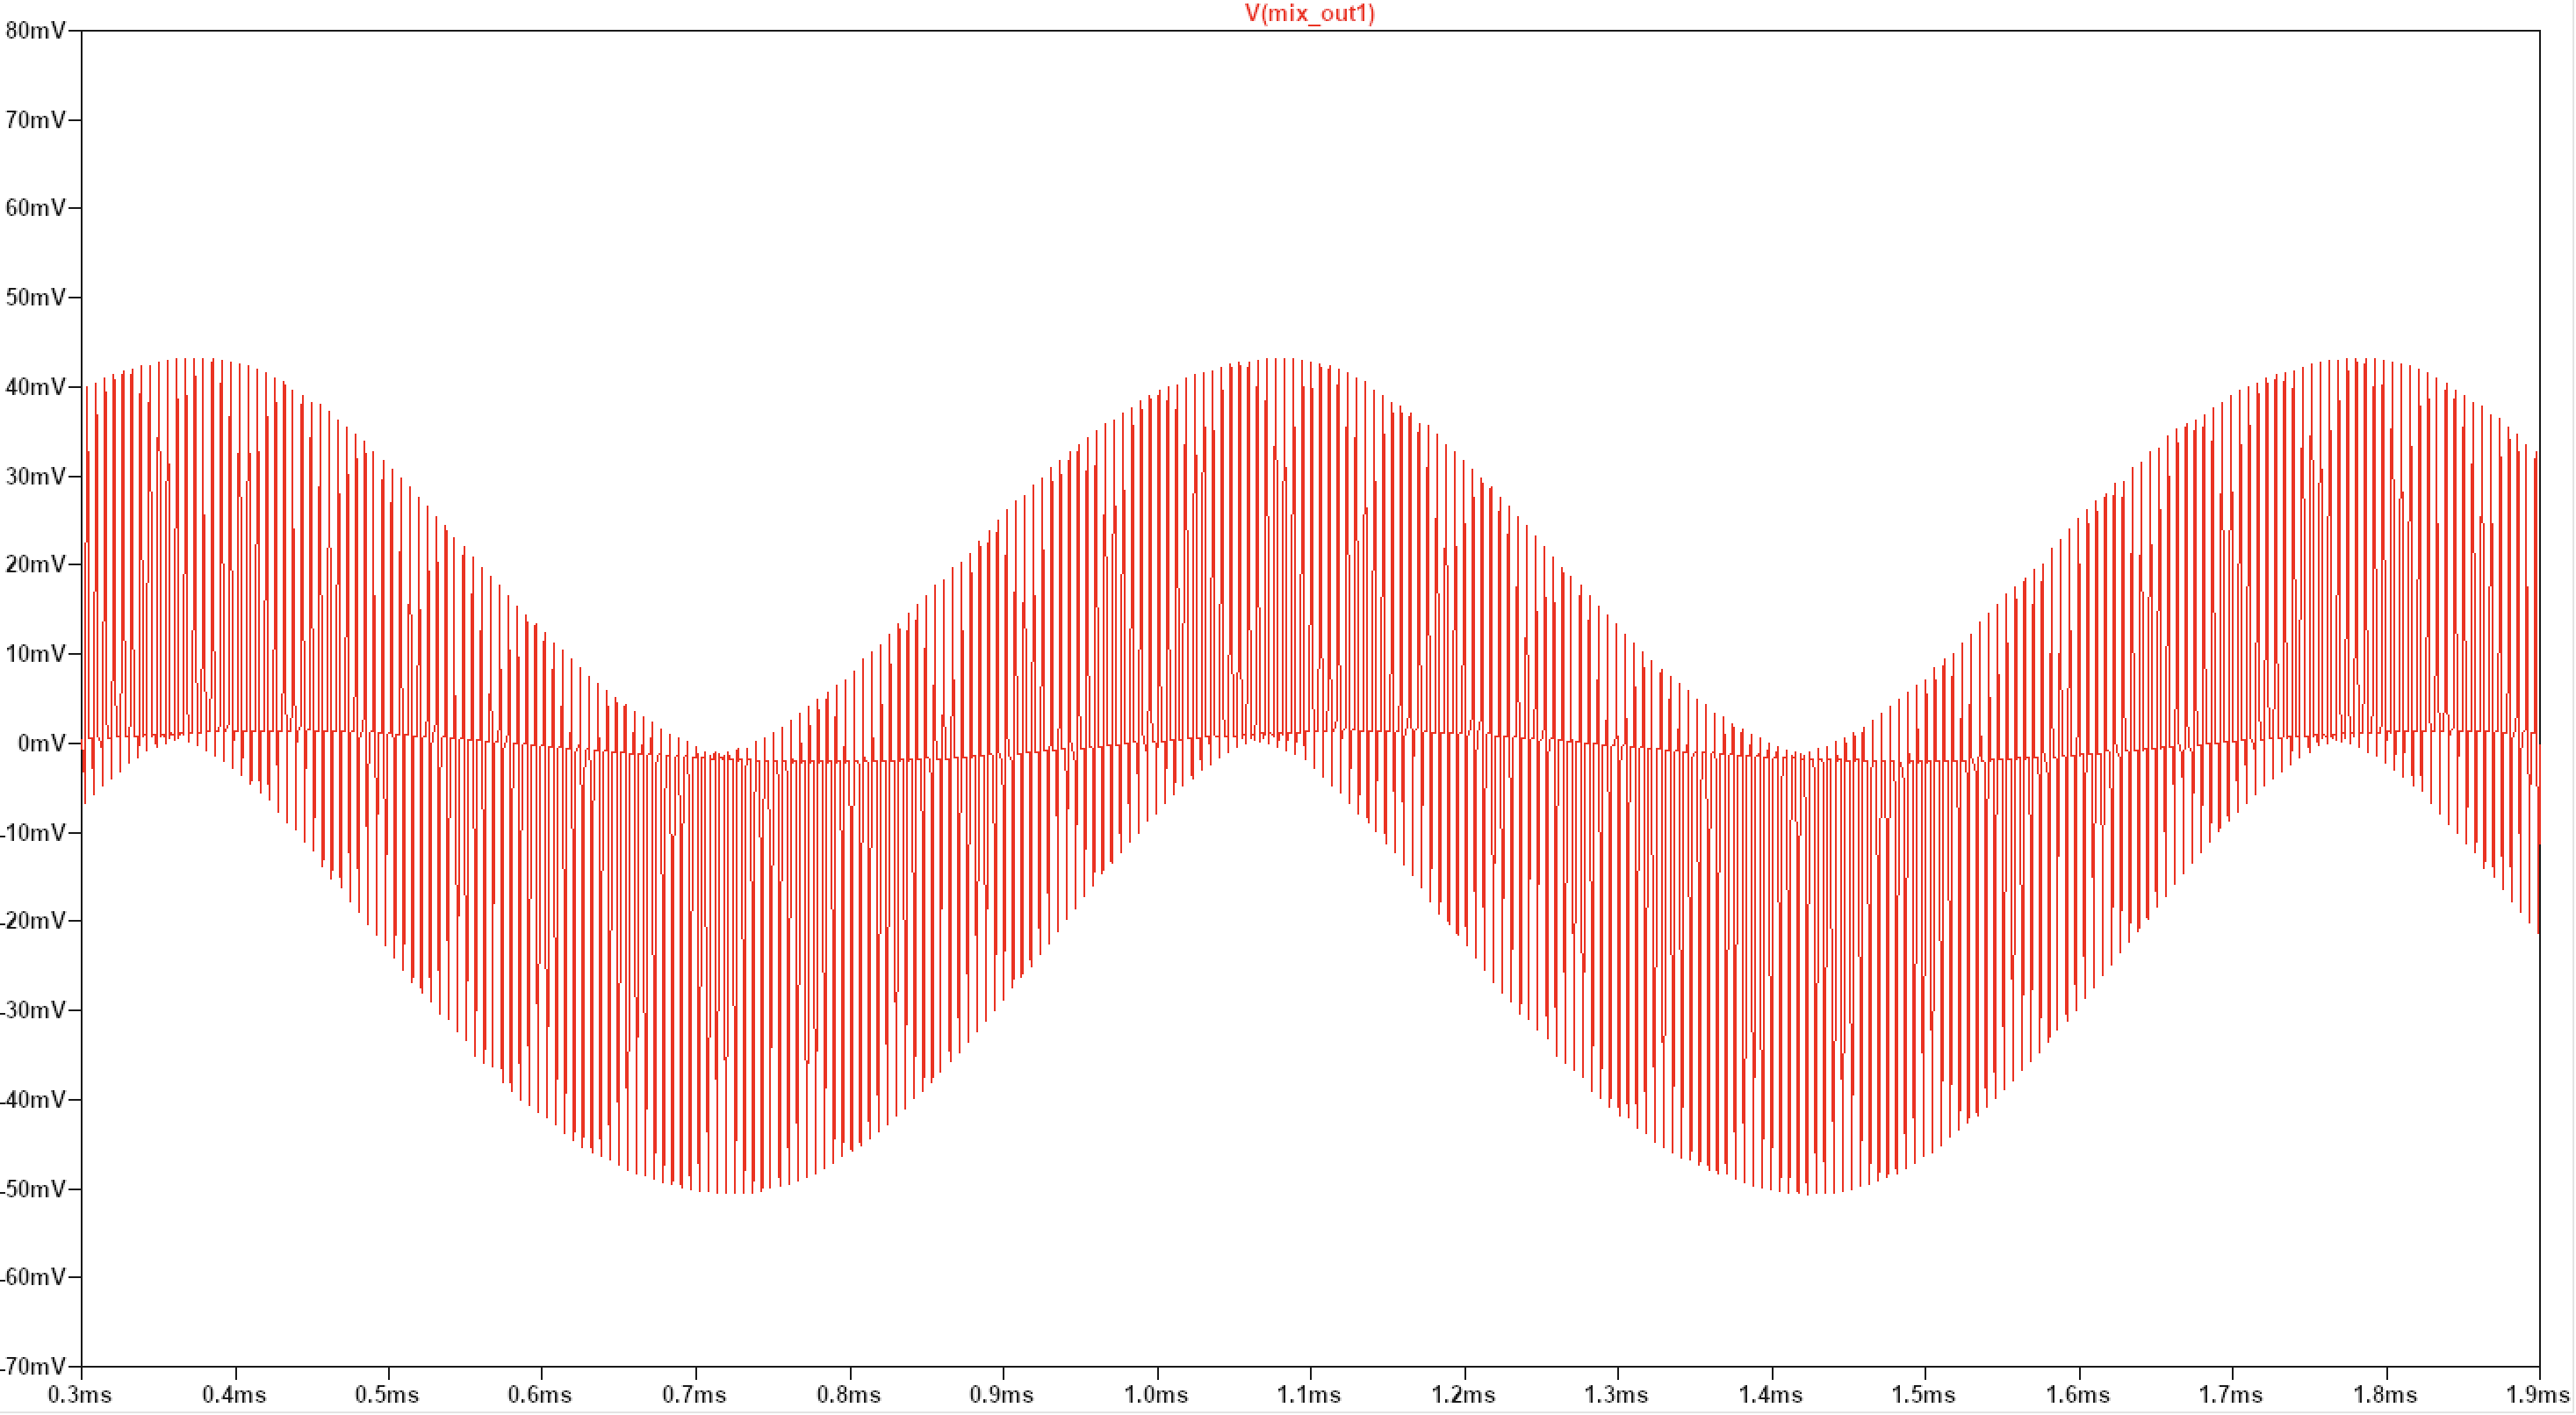
\includegraphics[width=\columnwidth]{images/172k-t.png}
        \caption{$f_{IN} = 172\text{ kHz}$ Transient}
    \end{subfigure}
    
    \vspace{0.3cm}
    \begin{subfigure}[b]{\columnwidth}
        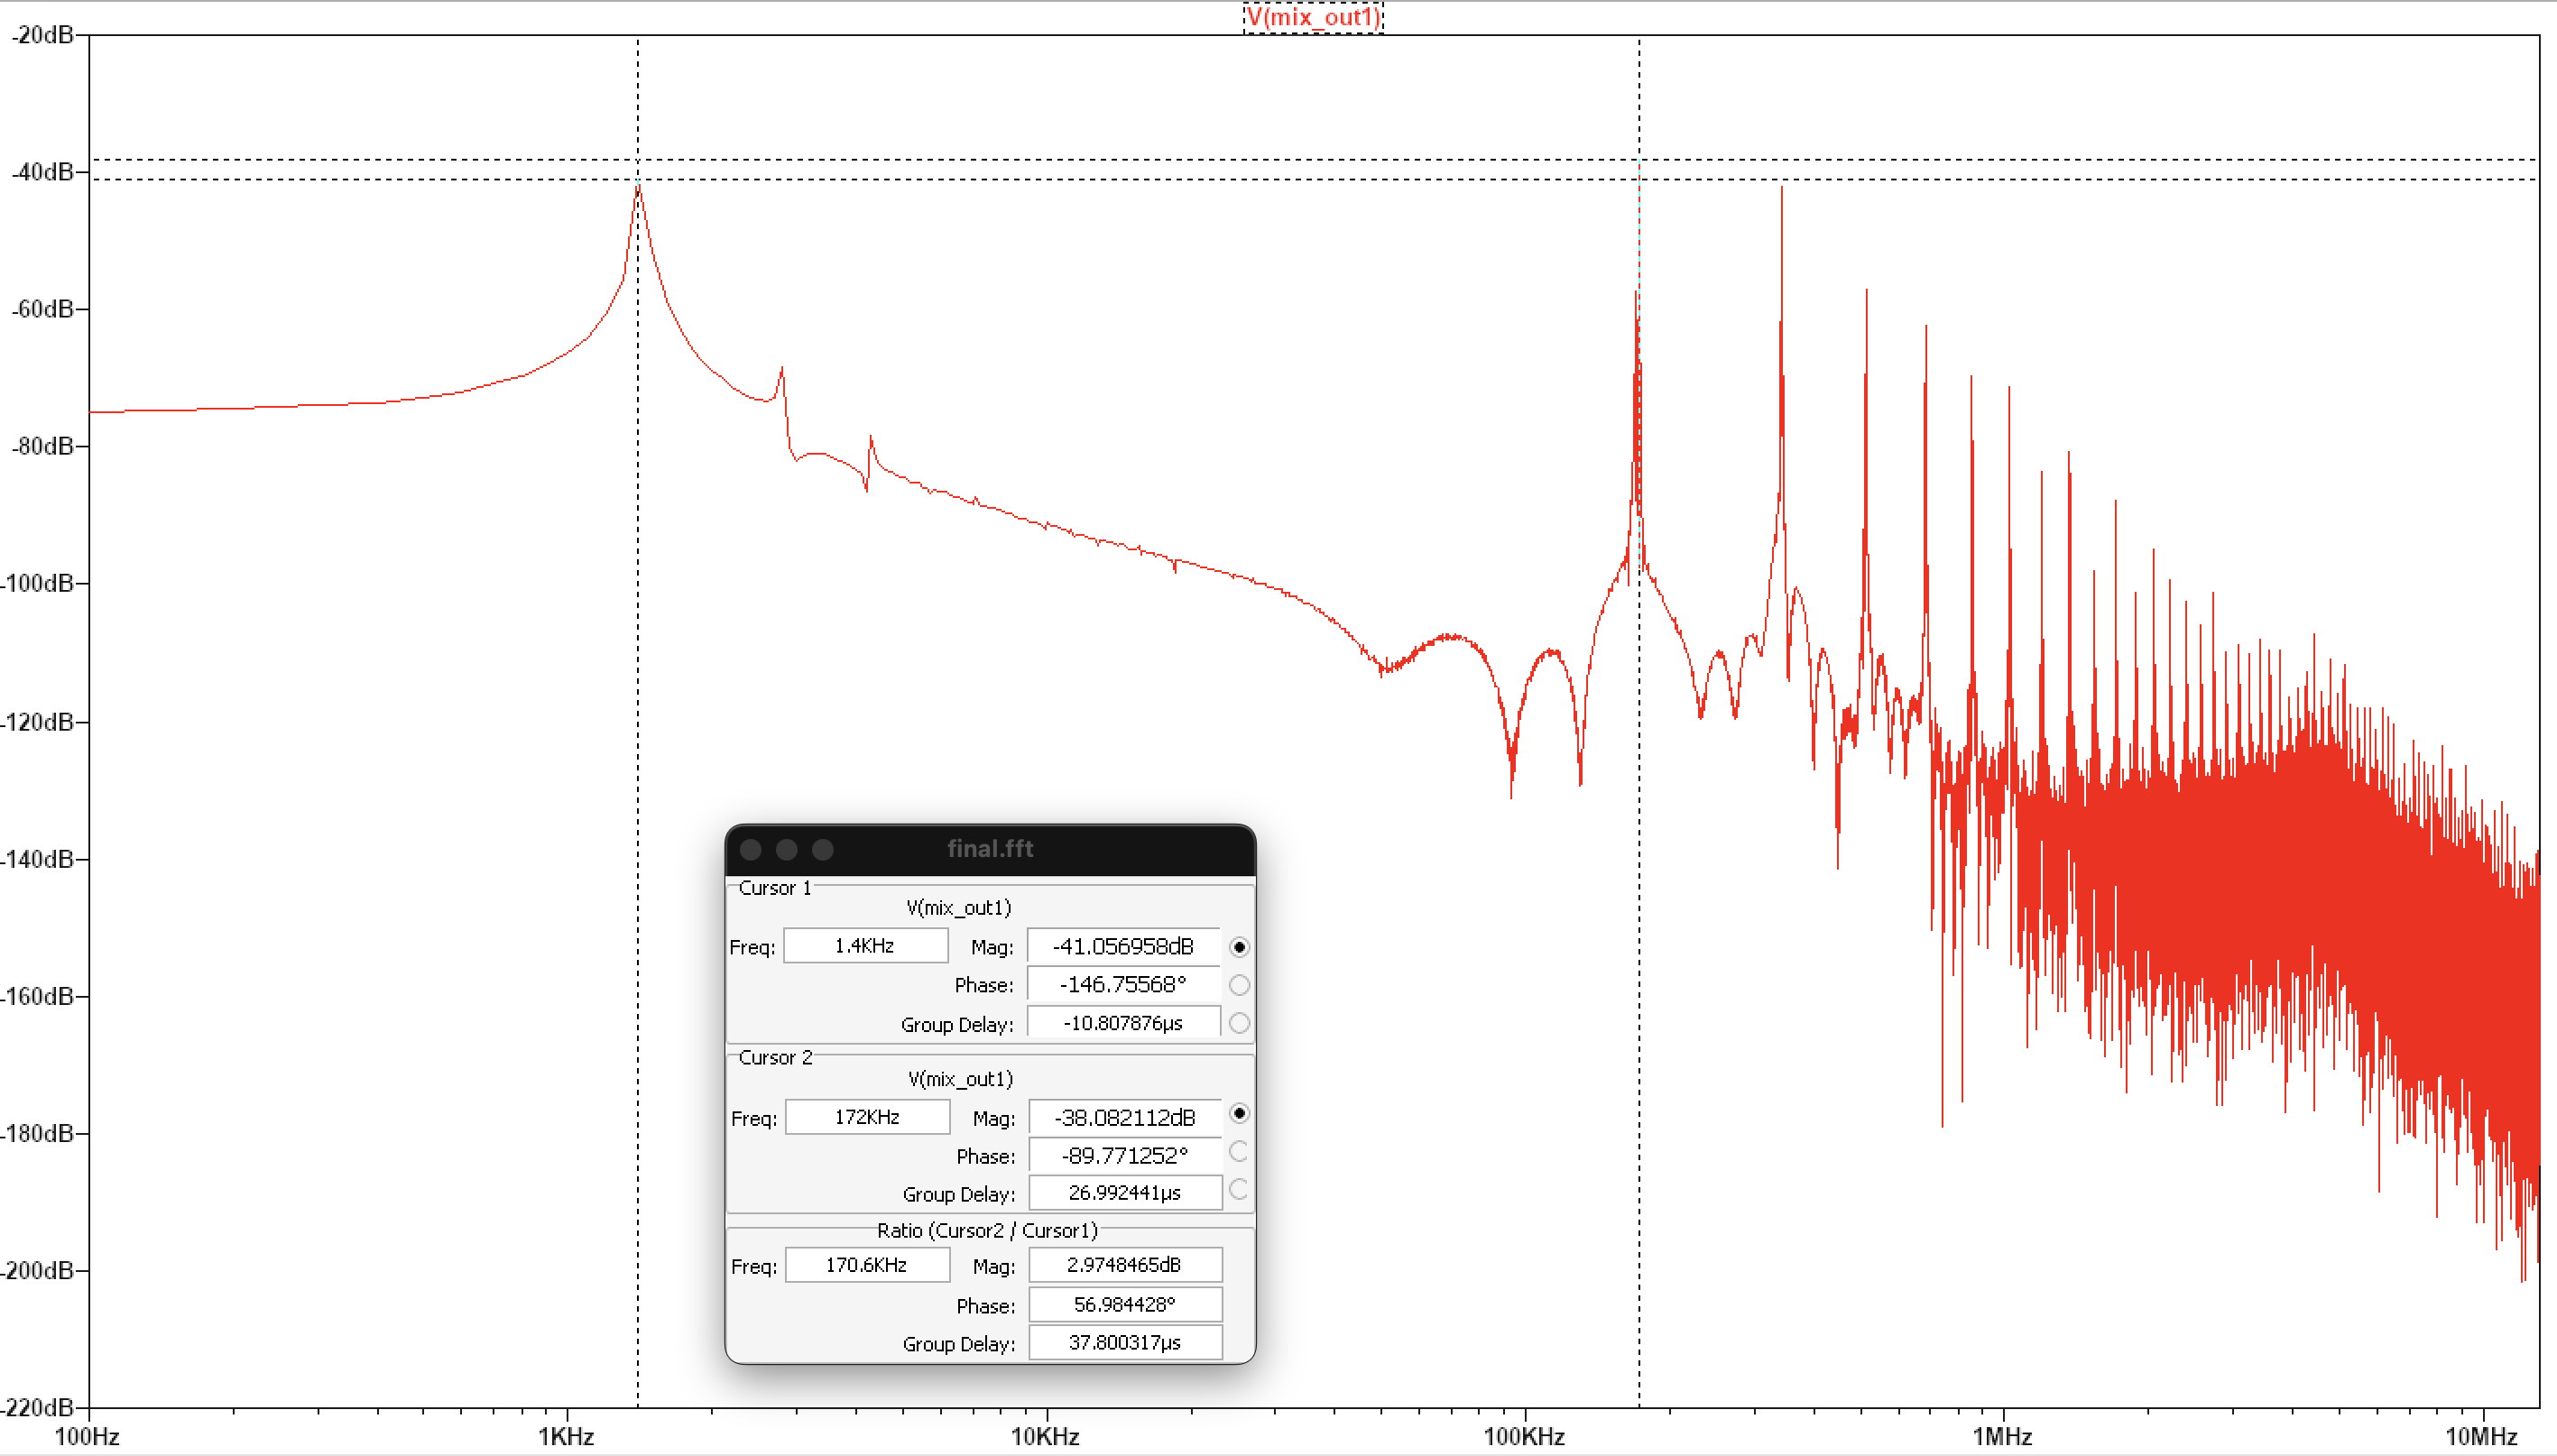
\includegraphics[width=\columnwidth]{images/172k-fft.png}
        \caption{$f_{IN} = 172\text{ kHz}$ FFT ($f_{IF} = 2\text{ kHz}$)}
    \end{subfigure}
    \caption{Mixer Output for $f_{IN} = 172\text{ kHz}$}
\end{figure}

\begin{figure}[htbp]
    \centering
    \begin{subfigure}[b]{\columnwidth}
        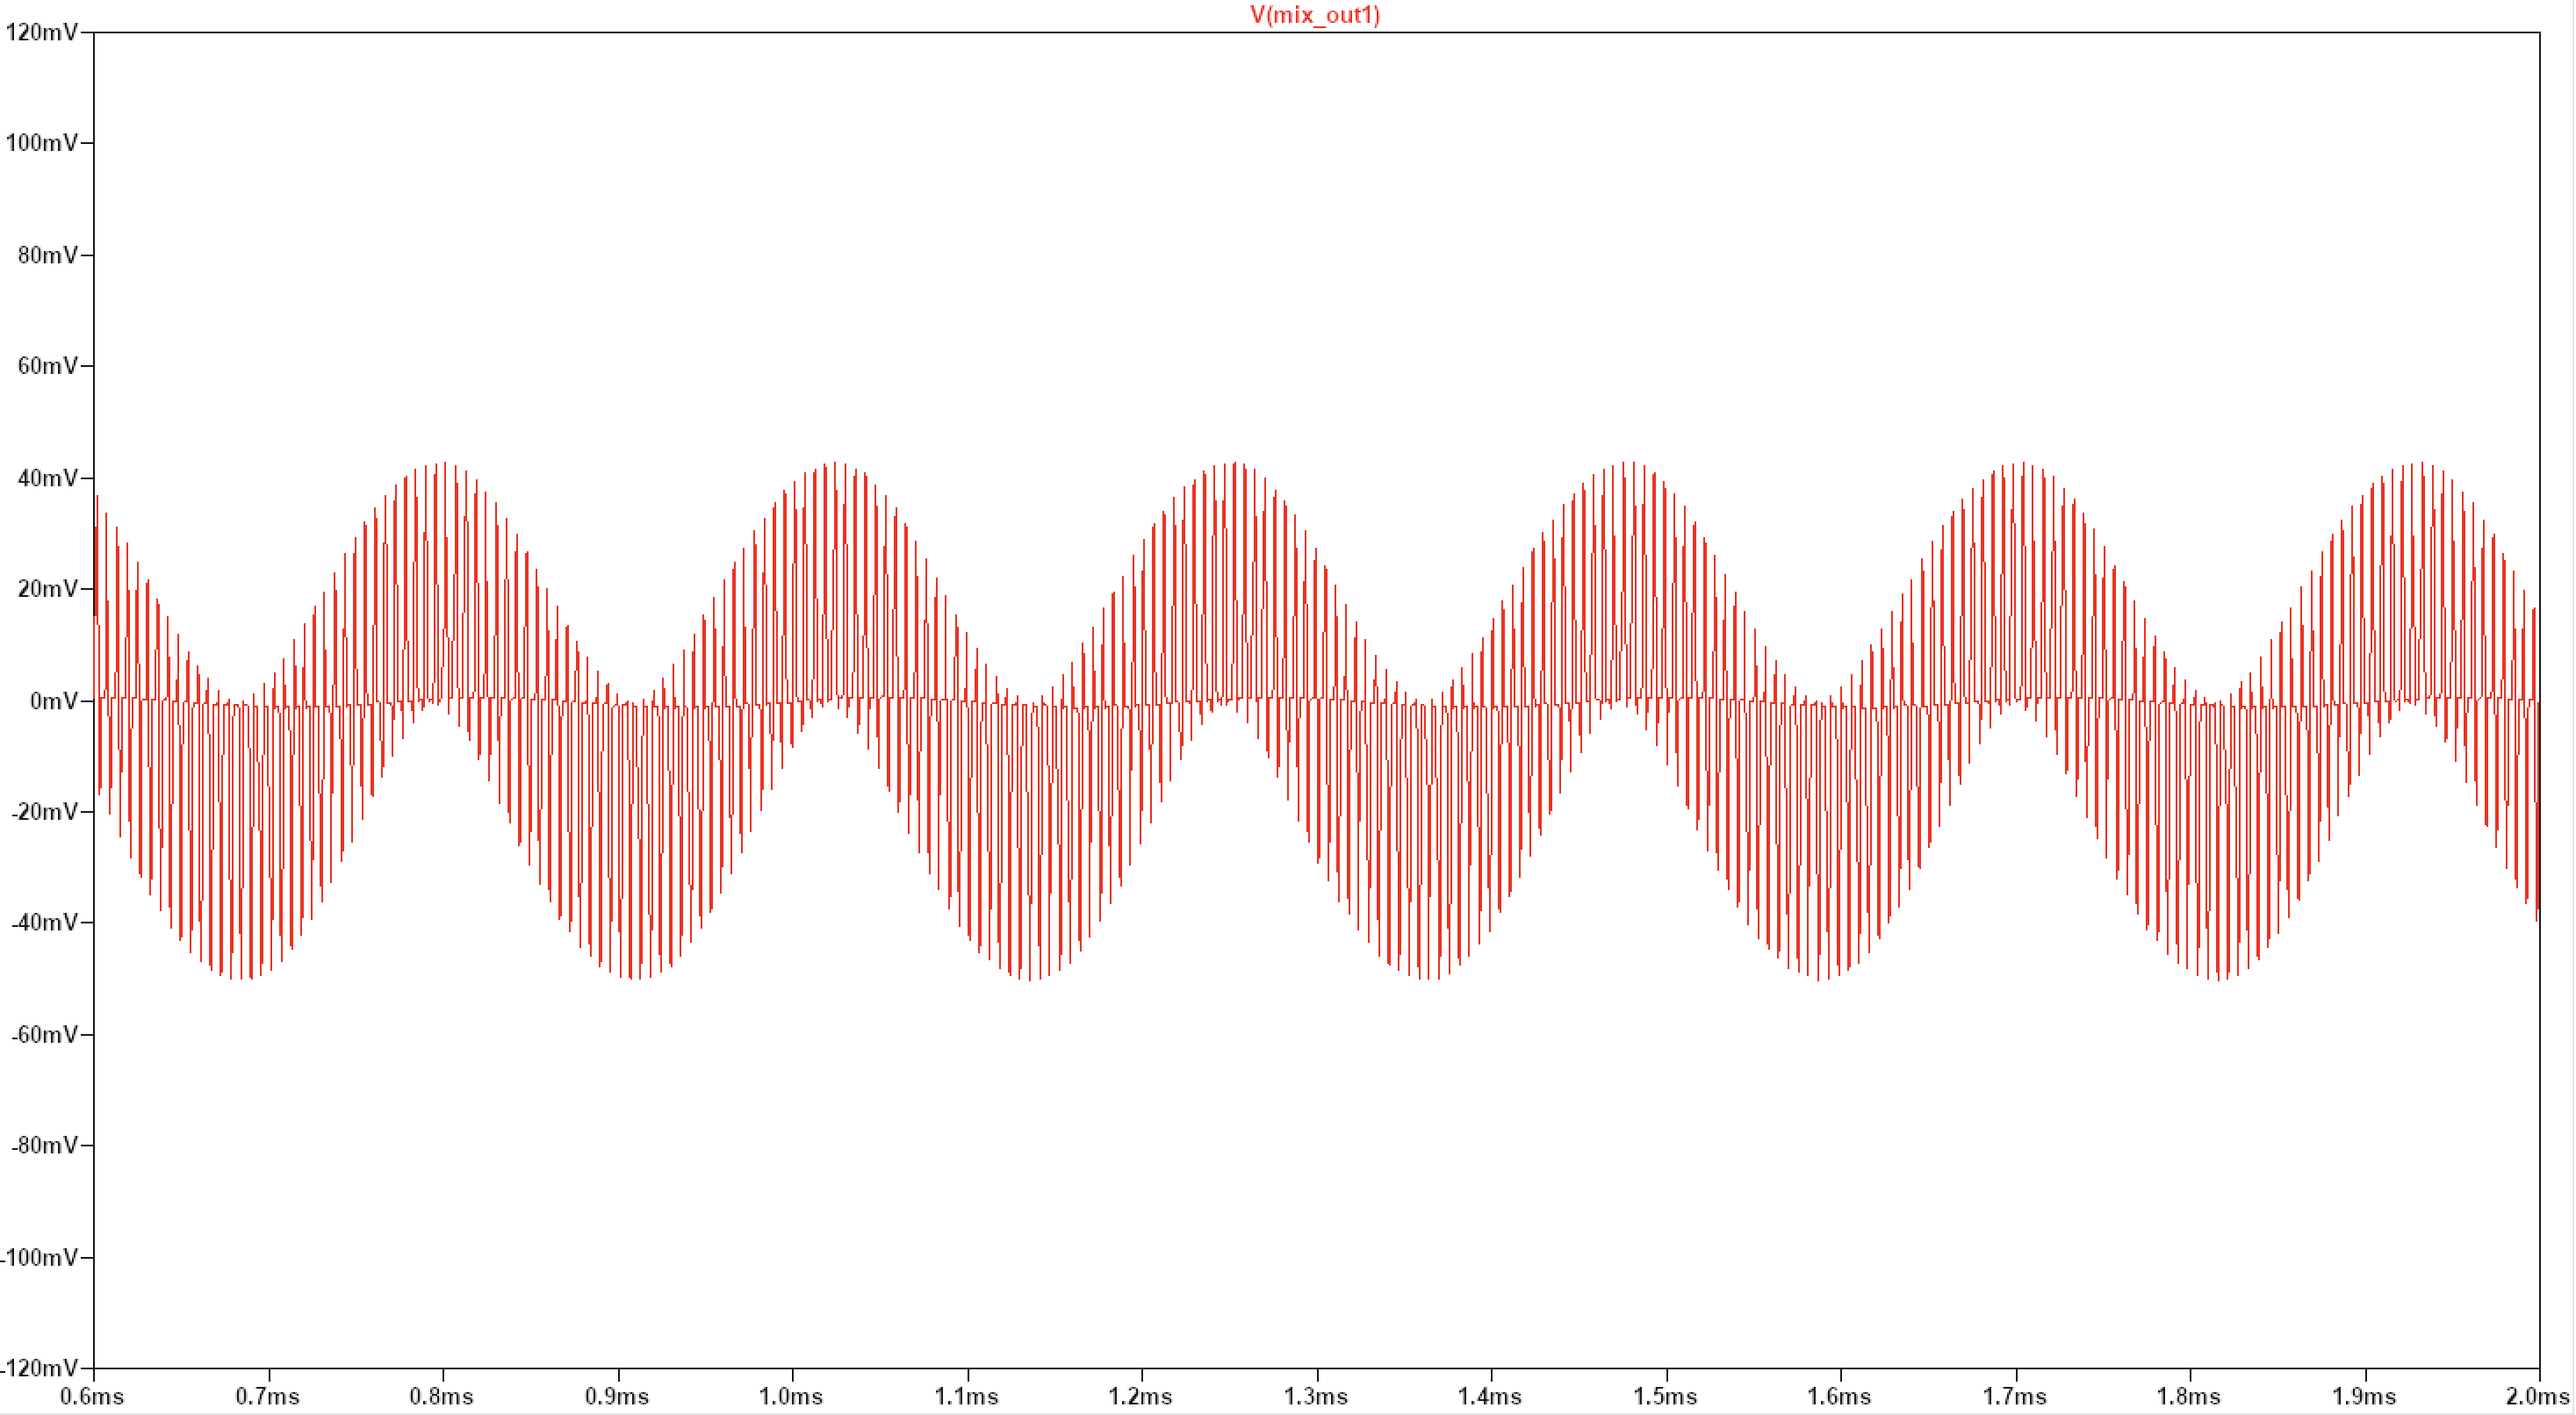
\includegraphics[width=\columnwidth]{images/175k-t.png}
        \caption{$f_{IN} = 175\text{ kHz}$ Transient}
    \end{subfigure}
    
    \vspace{0.3cm}
    \begin{subfigure}[b]{\columnwidth}
        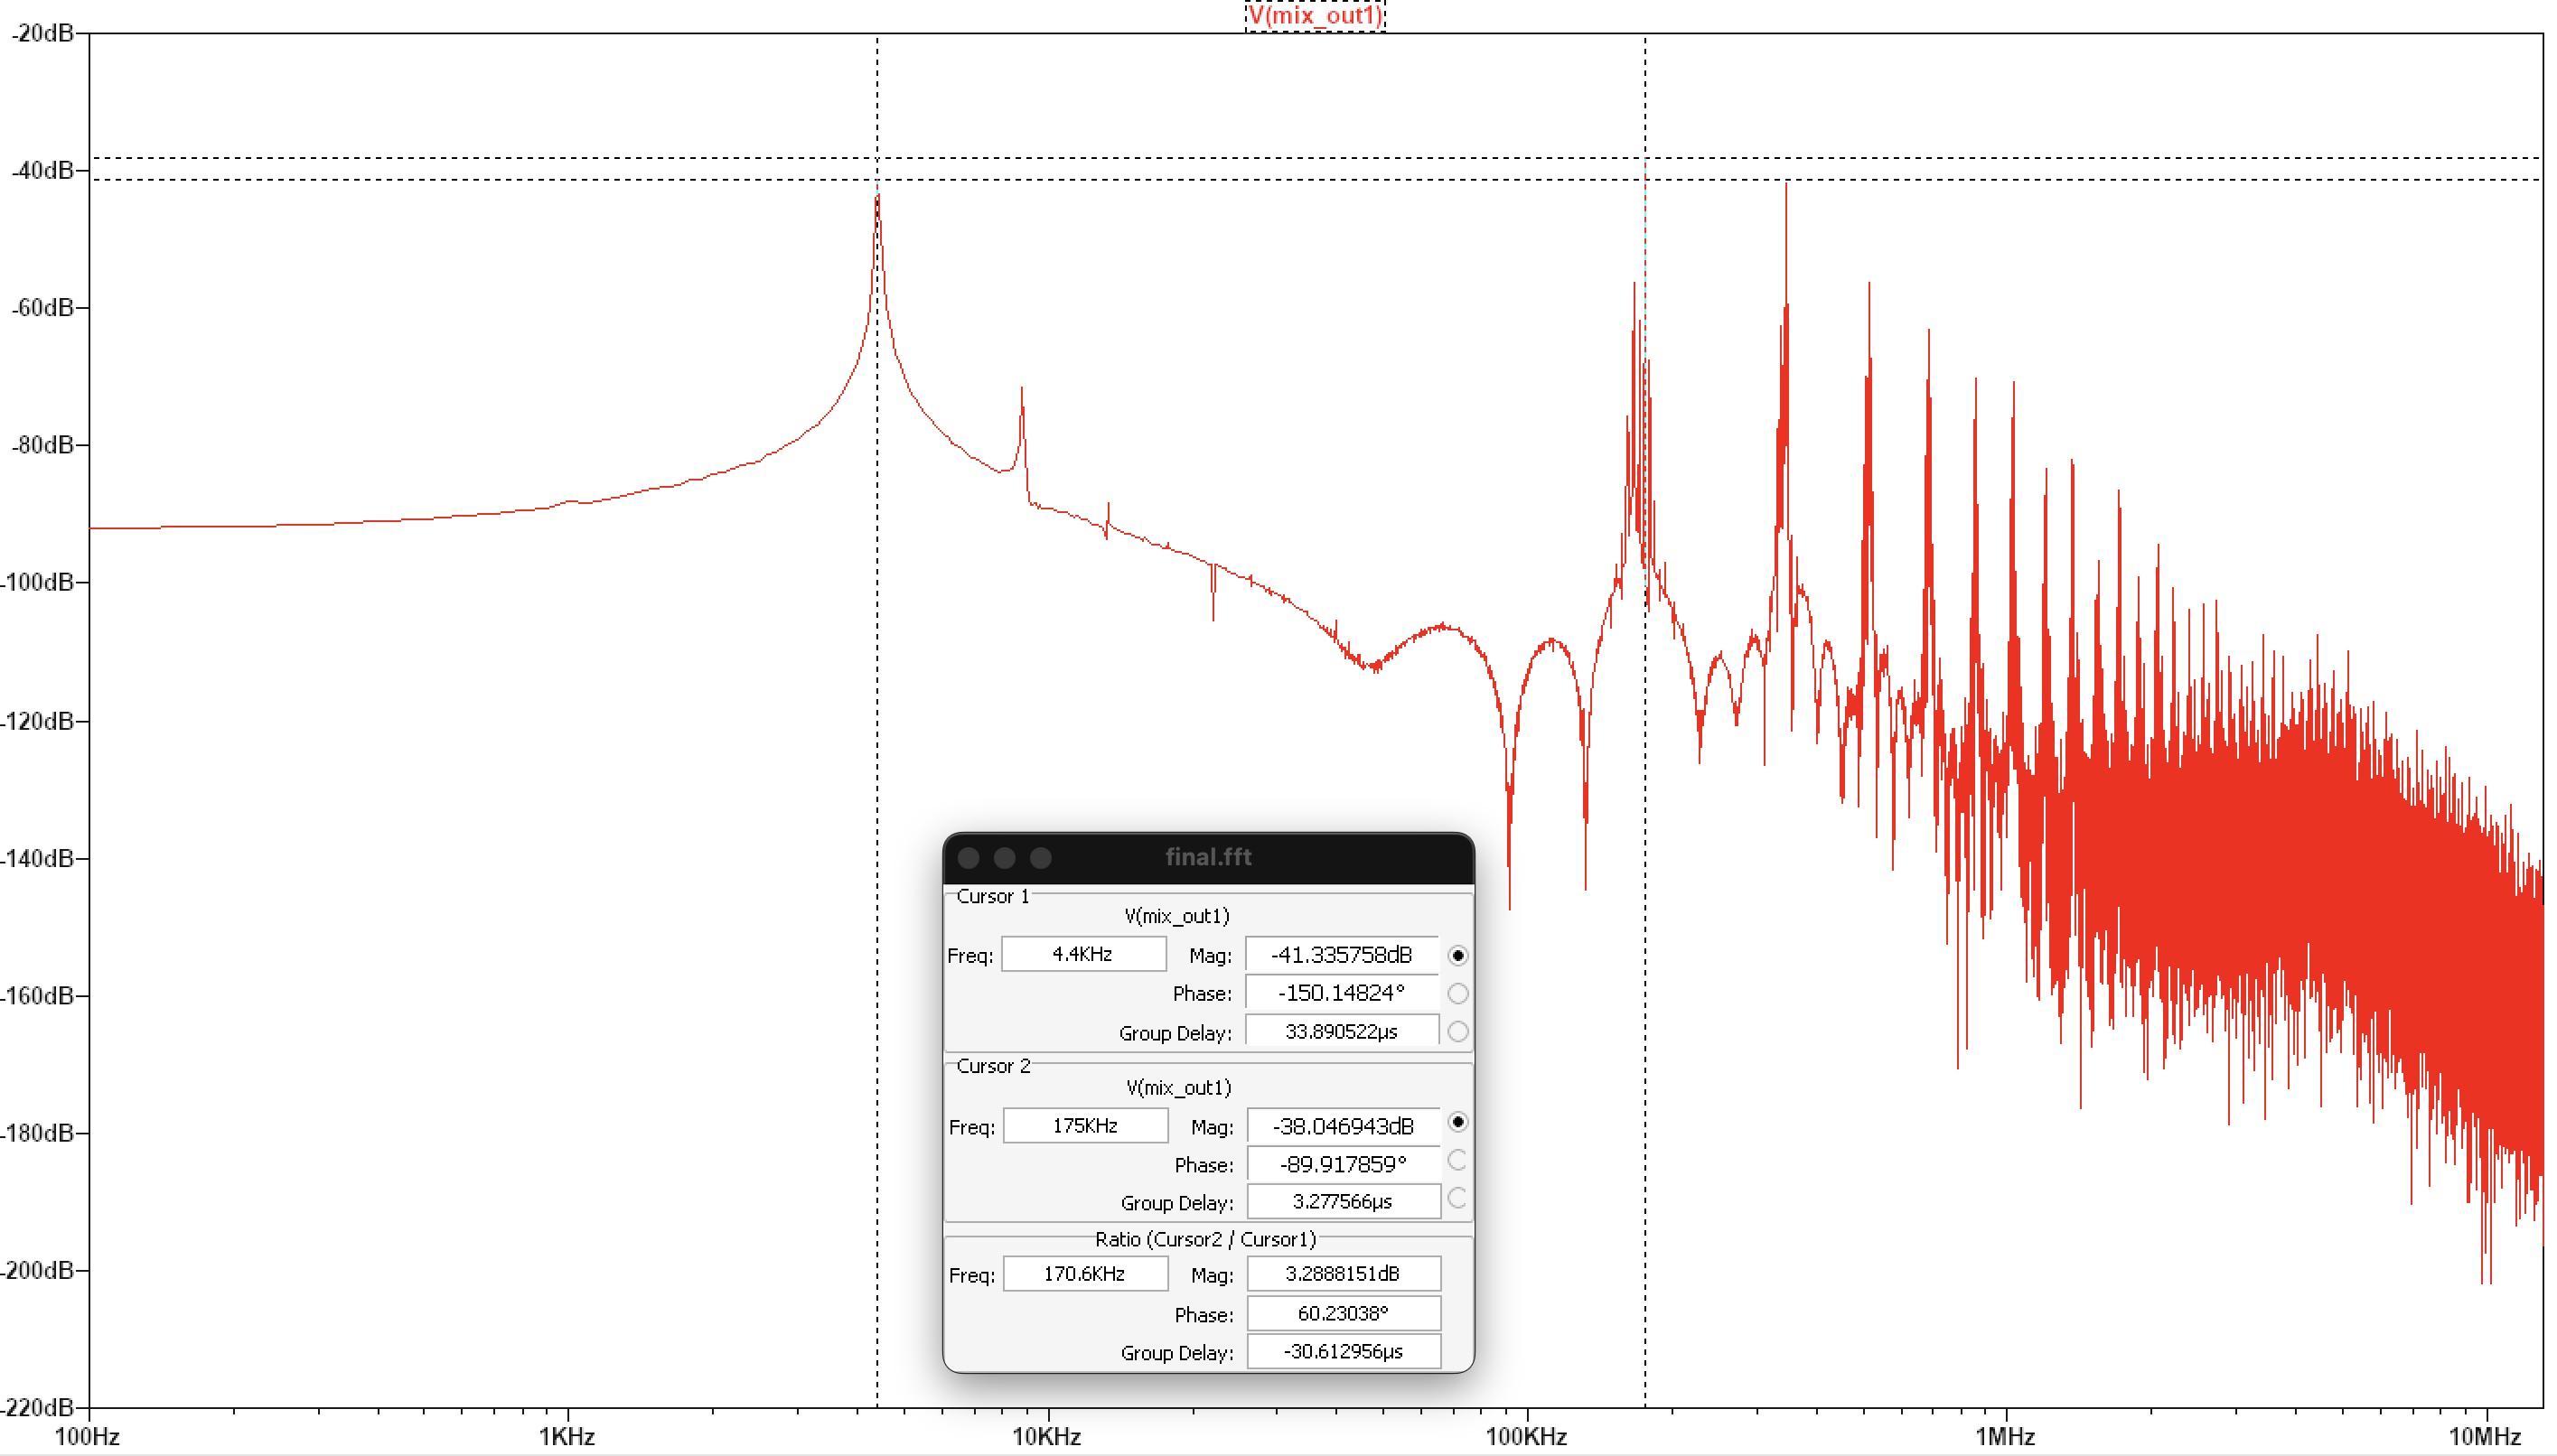
\includegraphics[width=\columnwidth]{images/175k-fft.png}
        \caption{$f_{IN} = 175\text{ kHz}$ FFT ($f_{IF} = 5\text{ kHz}$)}
    \end{subfigure}
    \caption{Mixer Output for $f_{IN} = 175\text{ kHz}$}
    \label{fig:mixer_sweep_above}
\end{figure}

\subsubsection{Explanation of Mixer Operation and Frequency Conversion}
Based on the transient and FFT plots presented above, the operation of the NMOS switch mixer can be summarized by the following key principles:

\begin{itemize}
    \item \textbf{Mathematical Downconversion:} The fundamental purpose of the mixer is to multiply the RF input ($f_{IN}$) with the local oscillator ($f_{OSC} = 170\text{ kHz}$). According to trigonometric identities, this multiplication creates two primary new frequency bands: the sum ($f_{OSC} + f_{IN}$) and the difference ($|f_{OSC} - f_{IN}|$).
    \item \textbf{The Intermediate Frequency (IF):} The difference component is the desired Intermediate Frequency ($f_{IF}$). As $f_{IN}$ is swept from $165\text{ kHz}$ to $175\text{ kHz}$, the resulting $f_{IF}$ is strictly the absolute difference from the $170\text{ kHz}$ carrier. For example, both $165\text{ kHz}$ and $175\text{ kHz}$ yield an identical $5\text{ kHz}$ IF envelope.
    \item \textbf{Time-Domain Envelopes:} In the transient plots, this $f_{IF}$ manifests as a slow, low-frequency amplitude modulation envelope riding over the high-frequency carrier. As $f_{IN}$ approaches $f_{OSC}$ (e.g., $169\text{ kHz}$ or $171\text{ kHz}$), the difference frequency shrinks to $1\text{ kHz}$, which is clearly visible as a much slower envelope period in the transient domain compared to the $165\text{ kHz}$ test.
    \item \textbf{FFT Spectral Verification:} The FFT plots definitively confirm this behavior. For every input frequency, a strong, distinct spectral peak appears exactly at the predicted $f_{IF}$ (e.g., at $f_{IN} = 168\text{ kHz}$, a prominent spike is observed exactly at $2\text{ kHz}$).
    \item \textbf{High-Frequency Spurious Content:} The transient waveforms also contain visible high-frequency "fuzz" or rapid switching noise. This consists of the sum frequency ($f_{OSC} + f_{IN} \approx 340\text{ kHz}$) and other LO harmonics ($3f_{OSC}$, etc.) caused by the square-wave nature of the NMOS switching. This high-frequency content dictates the strict necessity of the subsequent Low-Pass Filter (LPF) stage to isolate the pure IF tone.
\end{itemize}

\subsubsection{Hardware Realization and DSO Measurements}
To verify the mixer's theoretical performance in a physical environment, the NMOS switch mixer was constructed on a breadboard. Digital Storage Oscilloscope (DSO) measurements were taken to confirm that the physical hardware successfully downconverts the RF signal and produces the expected Intermediate Frequency (IF).

\begin{figure}[htbp]
    \centering
    \includegraphics[width=\columnwidth]{"images/mixer/WhatsApp Image 2026-04-17 at 21.17.00.jpeg"}
    \caption{Hardware Realization of the NMOS Switch Mixer.}
    \label{fig:mixer_hardware}
\end{figure}

\begin{figure}[htbp]
    \centering
    \begin{subfigure}[b]{\columnwidth}
        \includegraphics[width=\columnwidth]{"images/mixer/WhatsApp Image 2026-04-17 at 21.14.02.jpeg"}
        \caption{DSO Transient Capture ($f_{IN} = 175\text{ kHz}$).}
        \label{fig:mixer_dso_transient}
    \end{subfigure}
    
    \vspace{0.3cm}
    \begin{subfigure}[b]{\columnwidth}
        \includegraphics[width=\columnwidth]{"images/mixer/WhatsApp Image 2026-04-17 at 21.14.04 (1).jpeg"}
        \caption{DSO FFT Capture ($f_{IN} = 175\text{ kHz}$, showing $5\text{ kHz}$ peak).}
        \label{fig:mixer_dso_fft}
    \end{subfigure}
    \caption{Mixer Output DSO Measurements for $175\text{ kHz}$ Input.}
    \label{fig:mixer_dso_output}
\end{figure}

\begin{figure}[htbp]
    \centering
    \begin{subfigure}[b]{\columnwidth}
        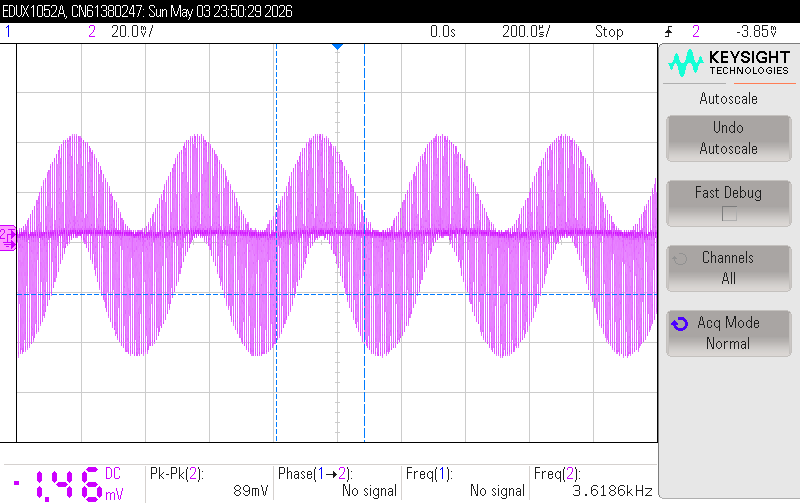
\includegraphics[width=\columnwidth]{images/mixer-img1.png}
        \caption{Mixer Output Measurement 1.}
        \label{fig:mixer_img1}
    \end{subfigure}
    
    \vspace{0.3cm}
    \begin{subfigure}[b]{\columnwidth}
        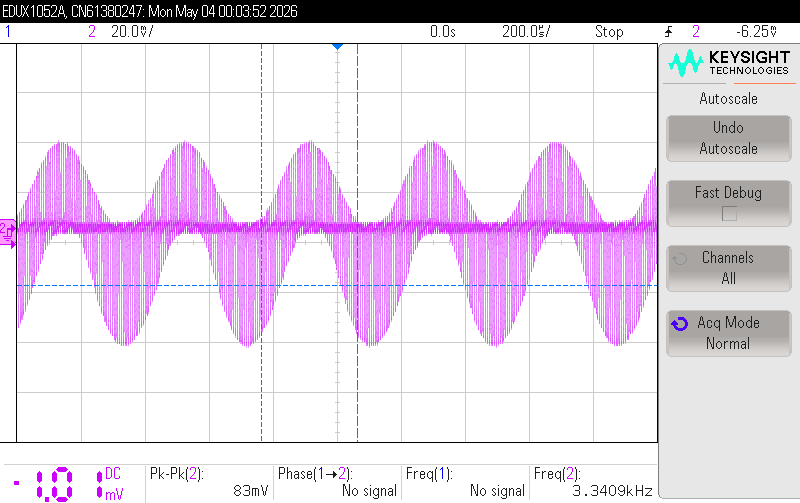
\includegraphics[width=\columnwidth]{images/mixer-img2.png}
        \caption{Mixer Output Measurement 2.}
        \label{fig:mixer_img2}
    \end{subfigure}
    \caption{Additional Mixer Output Measurements.}
    \label{fig:mixer_additional_outputs}
\end{figure}

The DSO captures for the $175\text{ kHz}$ input frequency perfectly mirror the LTSpice simulations. The transient waveform clearly displays the expected $5\text{ kHz}$ low-frequency modulation envelope. Furthermore, the FFT measurement provides definitive proof of downconversion, displaying a prominent spike at exactly $5\text{ kHz}$, successfully validating the hardware implementation.

\section{Low Pass Filter Design}
To extract the $5\text{ kHz}$ IF signal while sufficiently rejecting the $335\text{ kHz}$ sum component and mixer switching noise, a Low-Pass Filter (LPF) is required.

\begin{figure}[htbp]
    \centering
    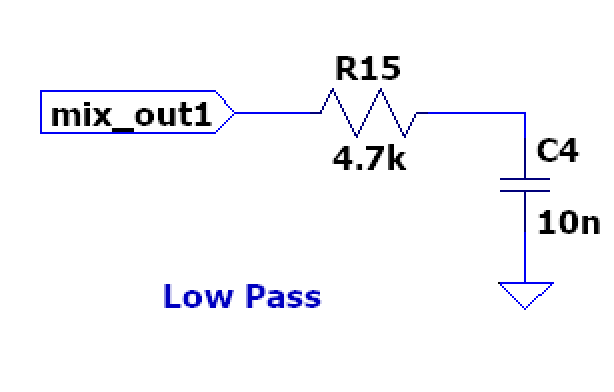
\includegraphics[width=0.6\linewidth]{images/lowpass.png}
    \caption{Low-Pass RC Filter Schematic.}
    \label{fig:lowpass}
\end{figure}

\subsection{Low-Pass RC Filter Design \& Calculations (Q4(a))}
The formula for the $-3\text{ dB}$ cut-off frequency ($f_c$) of a first-order low-pass RC filter is:
$$f_c = \frac{1}{2\pi R C}$$

\subsubsection{Given Component Values (Lab Practical)}
\begin{itemize}
    \item \textbf{Resistor ($R$):} $4.7\text{ k}\Omega = 4700\ \Omega$
    \item \textbf{Capacitor ($C$):} $10\text{ nF} = 10 \times 10^{-9}\text{ F}$
\end{itemize}

\subsubsection{Calculation of Actual Cut-off Frequency}
$$f_c = \frac{1}{2\pi \times 4700 \times (10 \times 10^{-9})}$$
$$f_c = \frac{1}{2\pi \times 4.7 \times 10^{-5}} = \frac{1}{0.00029531} \approx 3386.3\text{ Hz} \approx 3.39\text{ kHz}$$

\textbf{Note:} The question requests a design for a $3\text{ kHz}$ cut-off frequency. Utilizing standard available lab components ($4.7\text{ k}\Omega$ and $10\text{ nF}$), the cut-off frequency achieved is $3.39\text{ kHz}$, which serves as an excellent practical approximation for the desired target.

\subsubsection{Theoretical $3\text{ kHz}$ Design}
If the filter strictly needs exactly a $3\text{ kHz}$ cut-off frequency utilizing the available $10\text{ nF}$ capacitor, the ideal resistor value would instead be:
$$R = \frac{1}{2\pi \times 3000 \times 10 \times 10^{-9}} \approx 5.3\text{ k}\Omega$$

\subsection{LPF Simulation Results (Q4(b) \& Q4(c))}
The performance of the designed Low-Pass Filter was simulated to observe its time-domain and frequency-domain characteristics.

\begin{figure}[htbp]
    \centering
    \begin{subfigure}[b]{\columnwidth}
        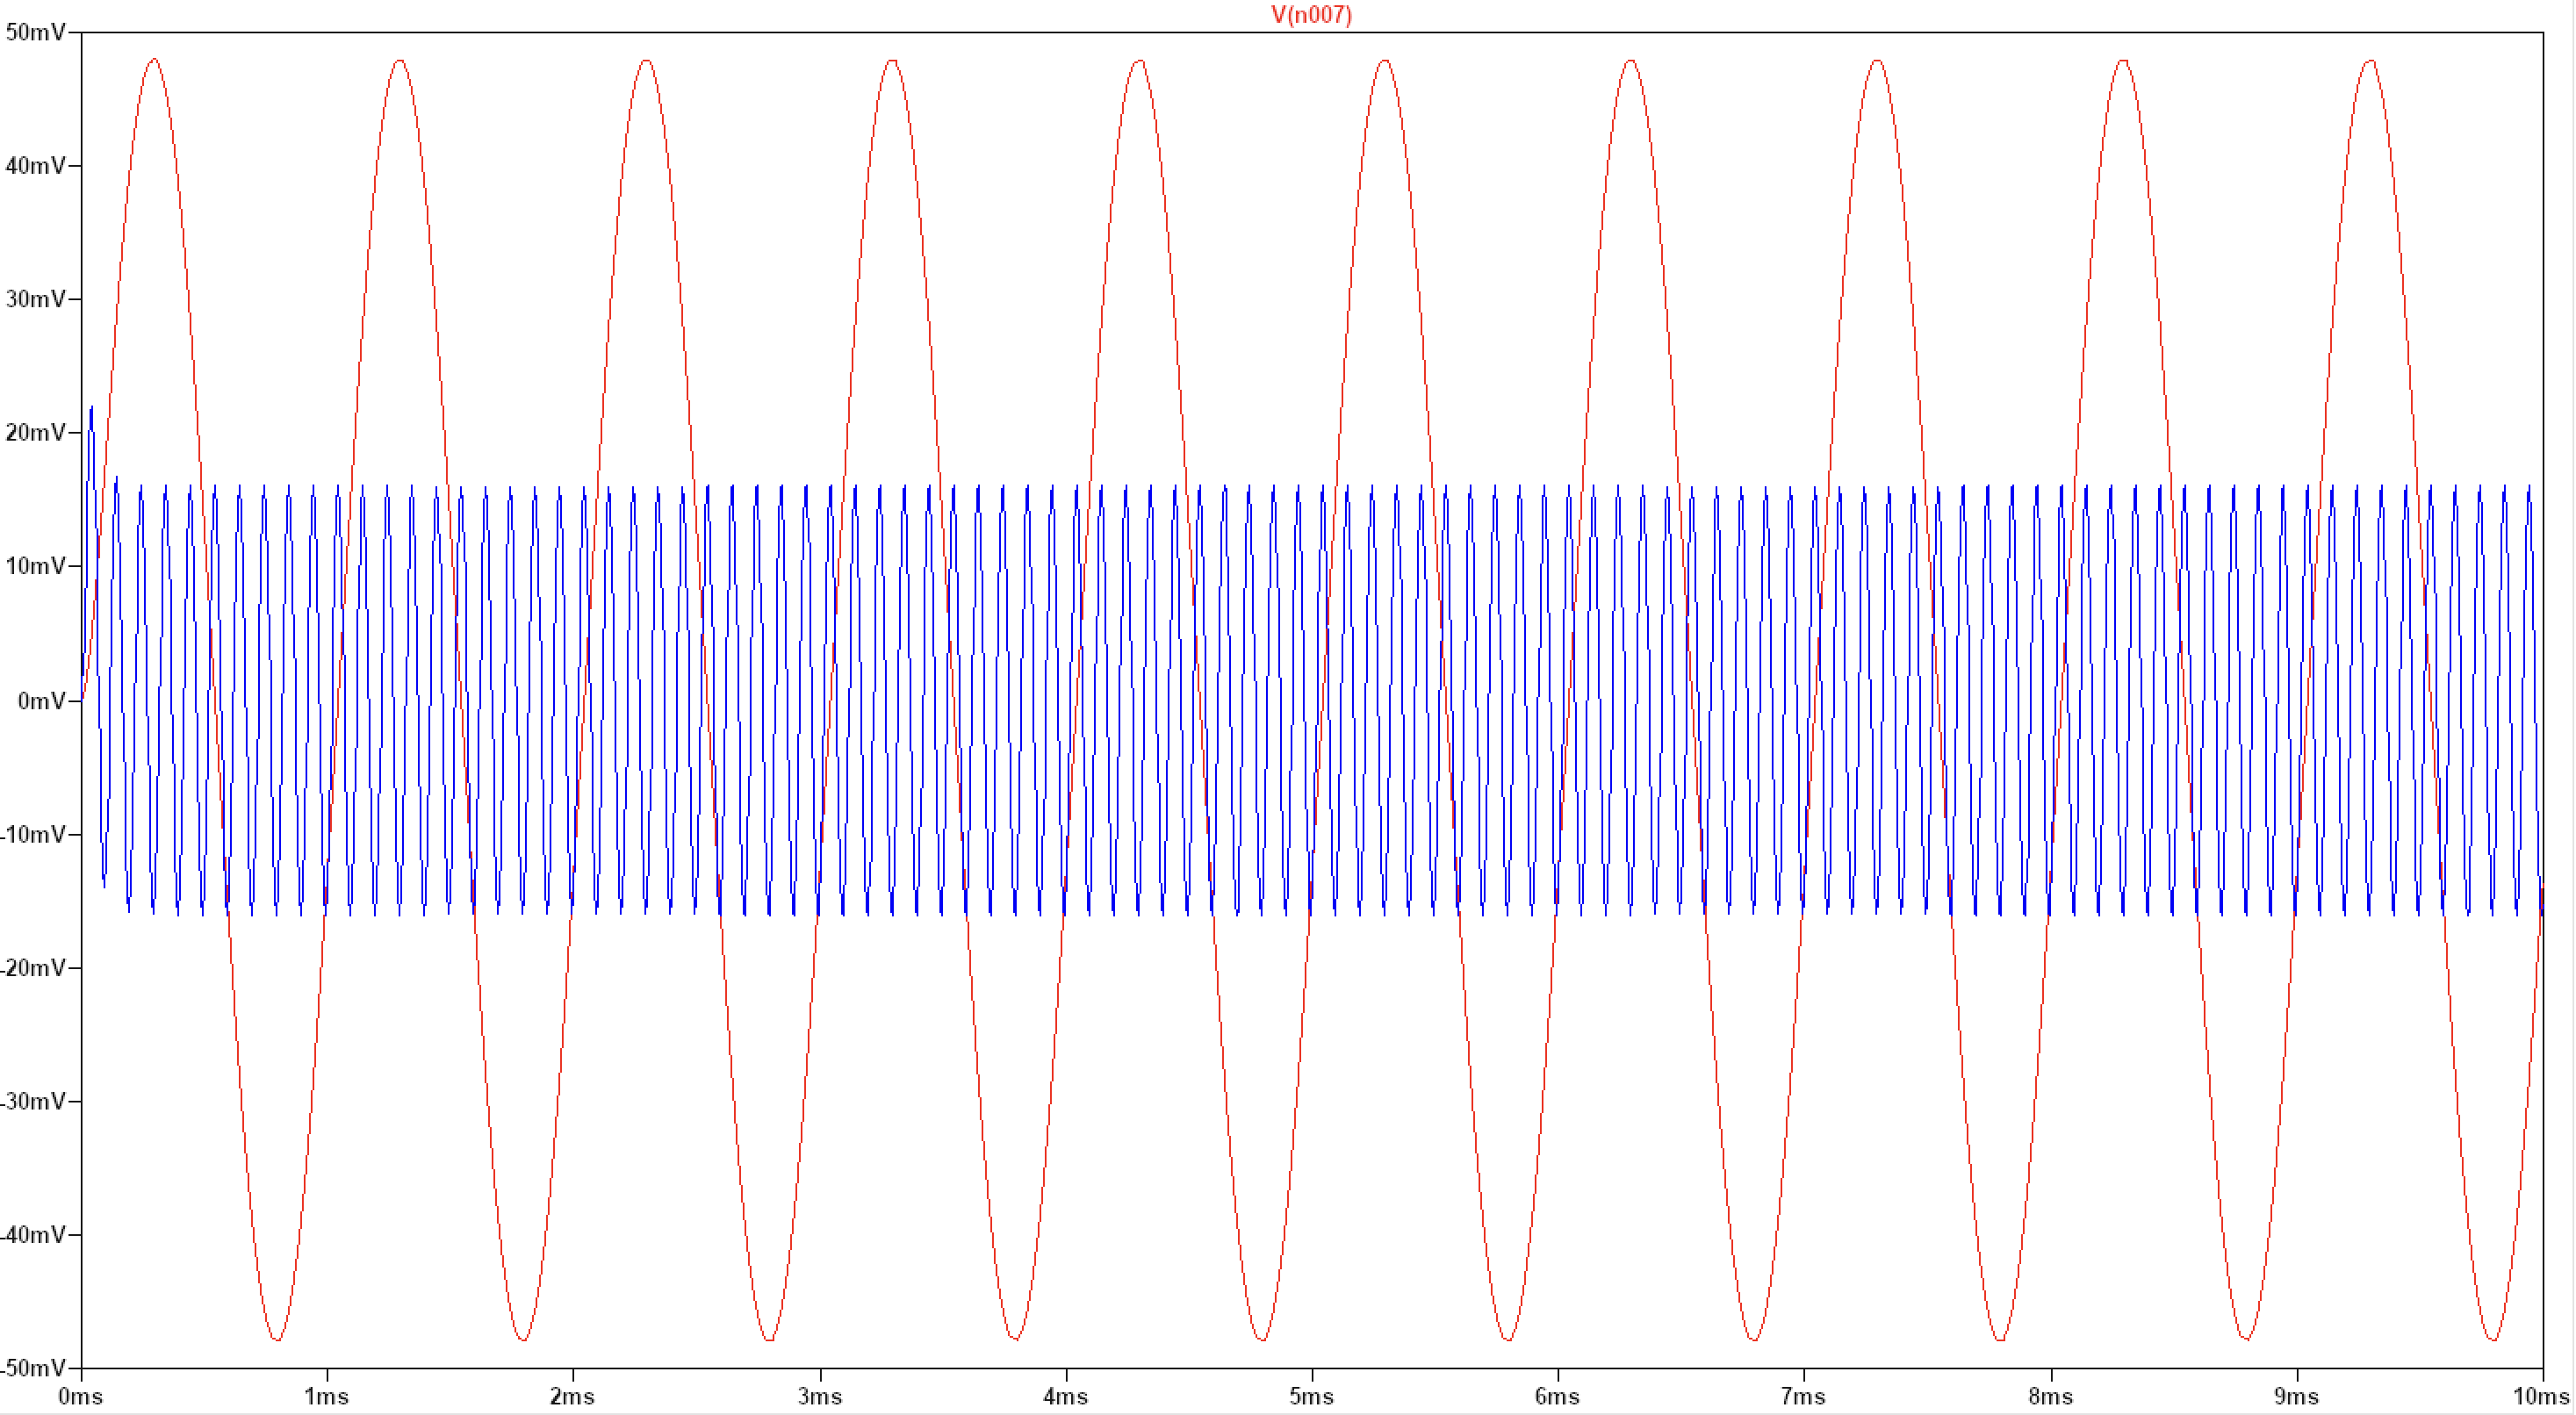
\includegraphics[width=\columnwidth]{images/LPF1-transient.png}
        \caption{Transient Response of the LPF.}
        \label{fig:lpf1_transient}
    \end{subfigure}
    
    \vspace{0.3cm}
    \begin{subfigure}[b]{\columnwidth}
        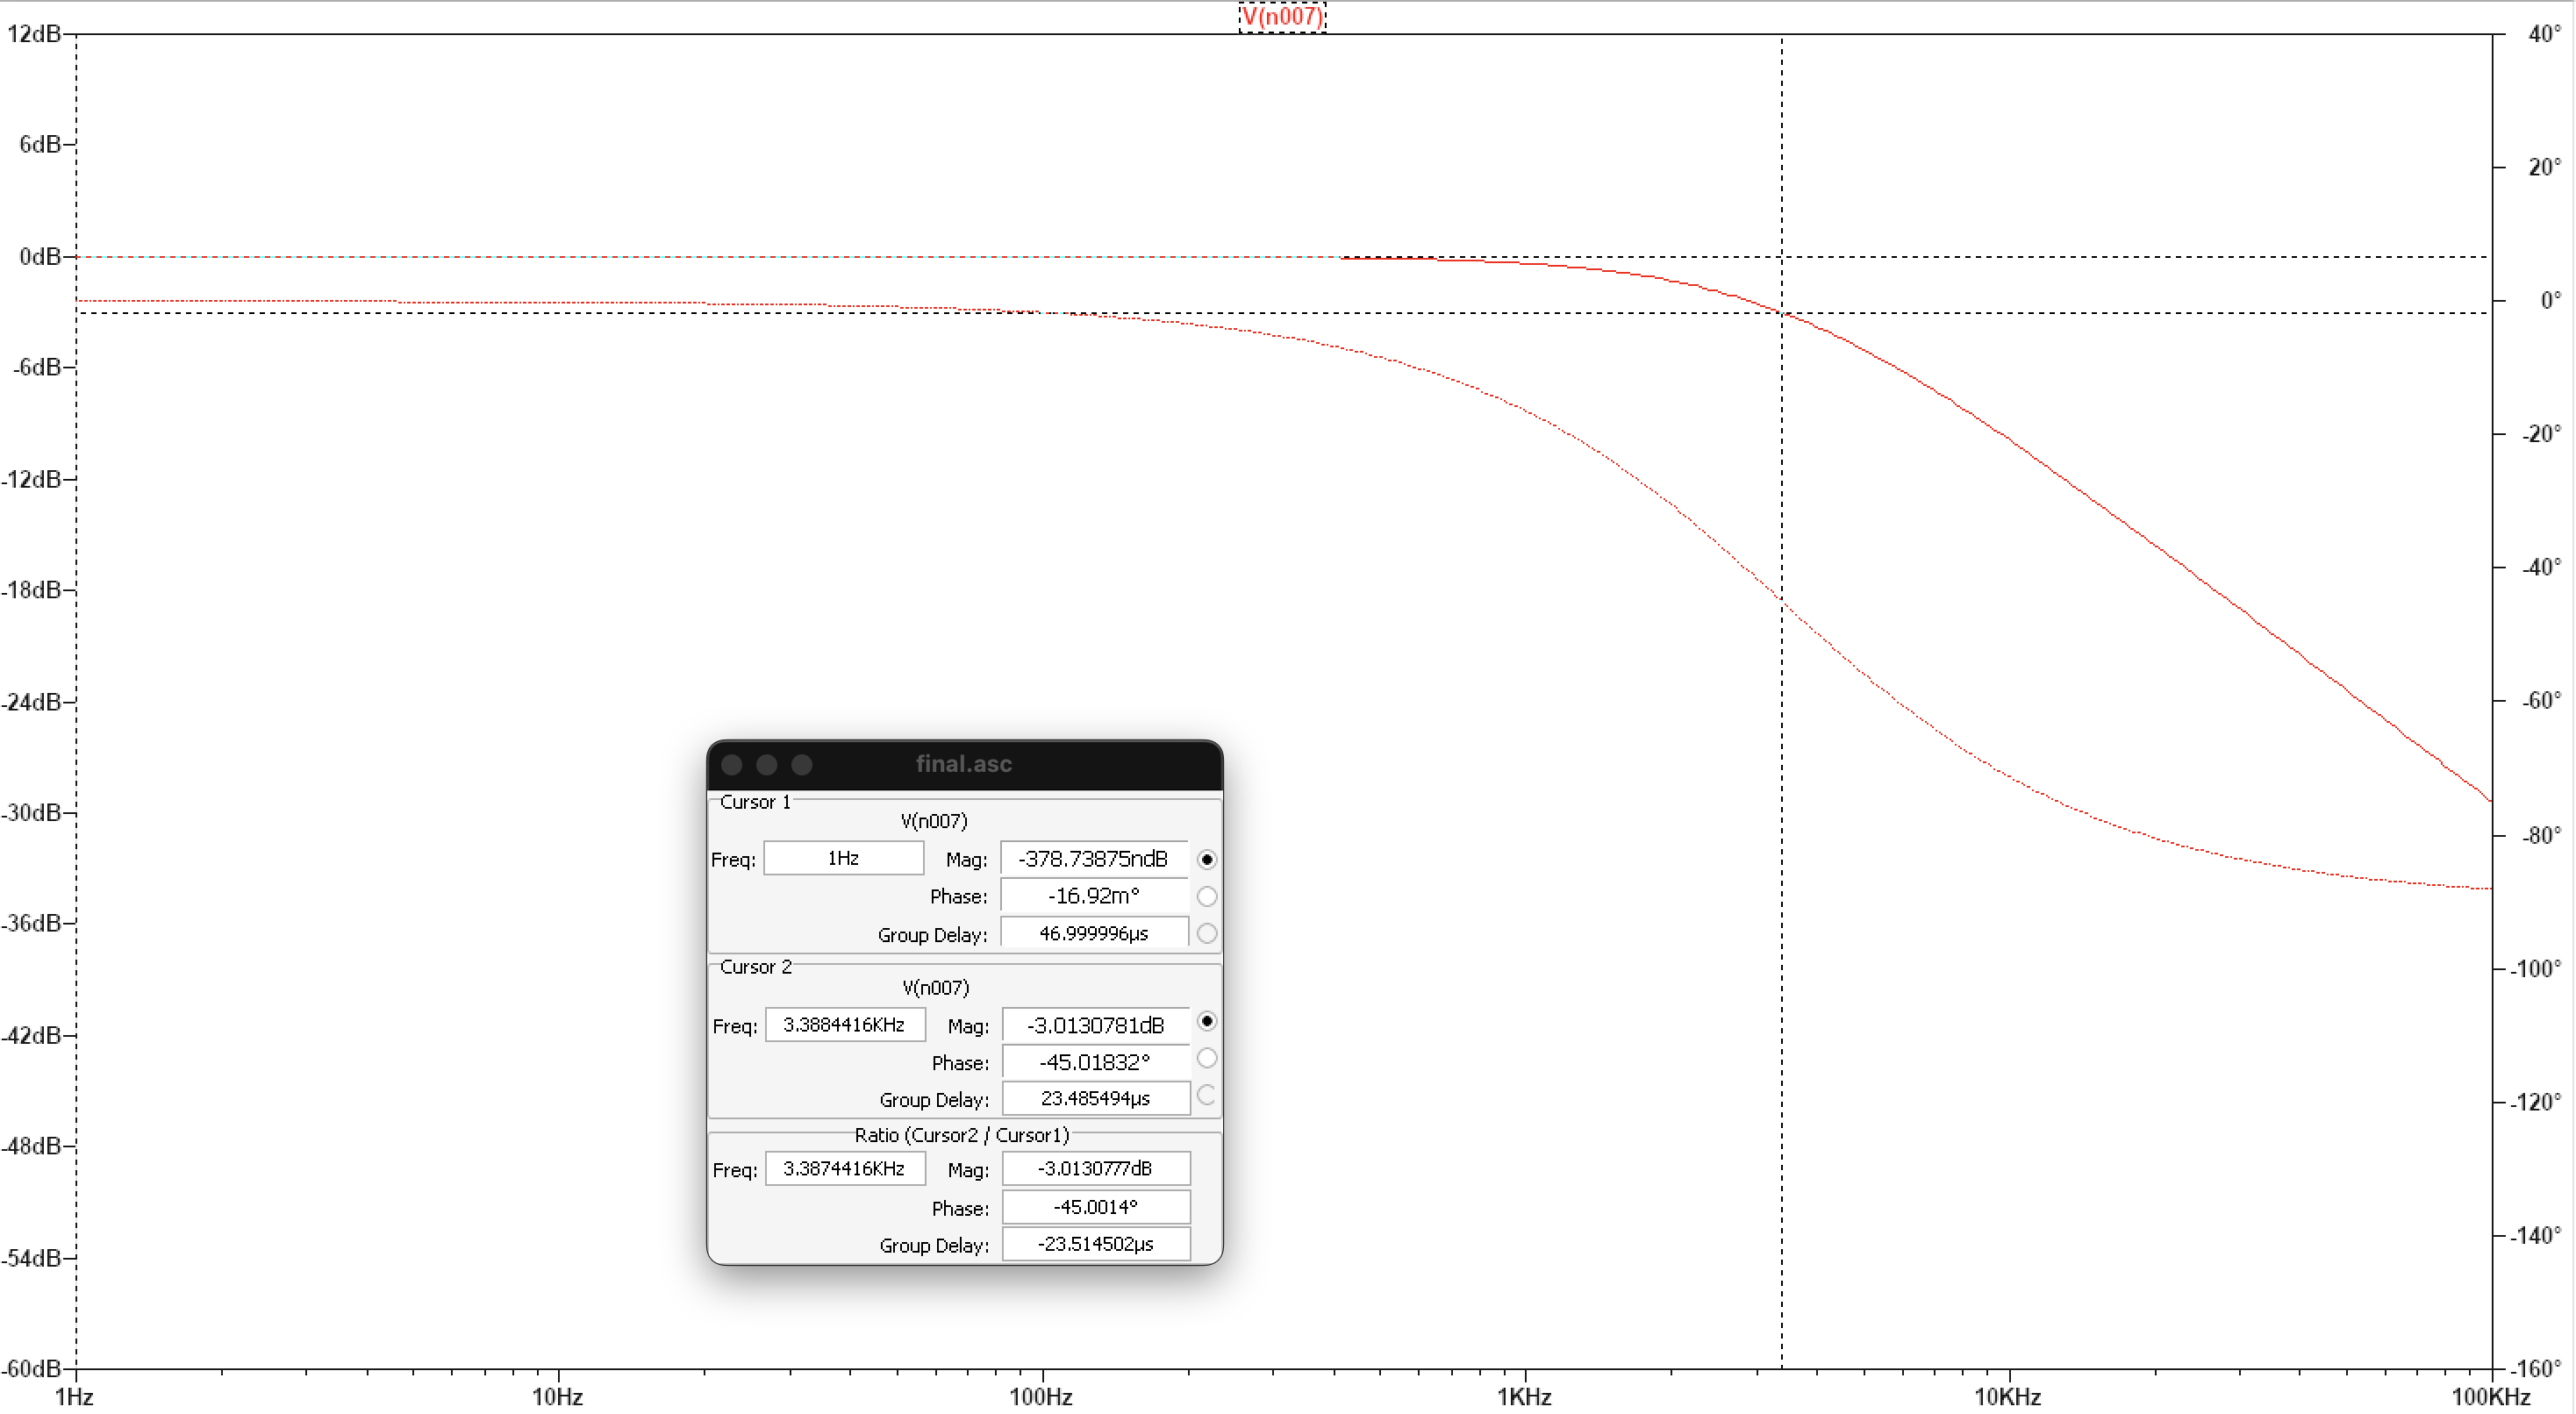
\includegraphics[width=\columnwidth]{images/LPF1-FFT.png}
        \caption{FFT Spectrum of the LPF Output.}
        \label{fig:lpf1_fft}
    \end{subfigure}
    \caption{Low-Pass Filter Simulation Results (Transient and FFT).}
    \label{fig:lpf_sim_results}
\end{figure}

The transient plot (Fig. \ref{fig:lpf1_transient}) demonstrates the successful extraction of the low-frequency envelope (the IF signal). The high-frequency switching noise and sum-frequency components from the mixer have been heavily attenuated by the RC network. The FFT (Fig. \ref{fig:lpf1_fft}) visually confirms this filtering action by displaying a strong, dominant peak at the downconverted IF, with the unwanted higher-order harmonics suppressed below the noise floor.

\subsection{Hardware Realization and Measurement (Q4(d))}
The designed Low-Pass Filter was physically realized in the laboratory to verify its real-world performance against the theoretical design. Measurements were taken using an oscilloscope to capture the transient responses and the overall AC frequency response.

\begin{figure}[htbp]
    \centering
    \begin{subfigure}[b]{\columnwidth}
        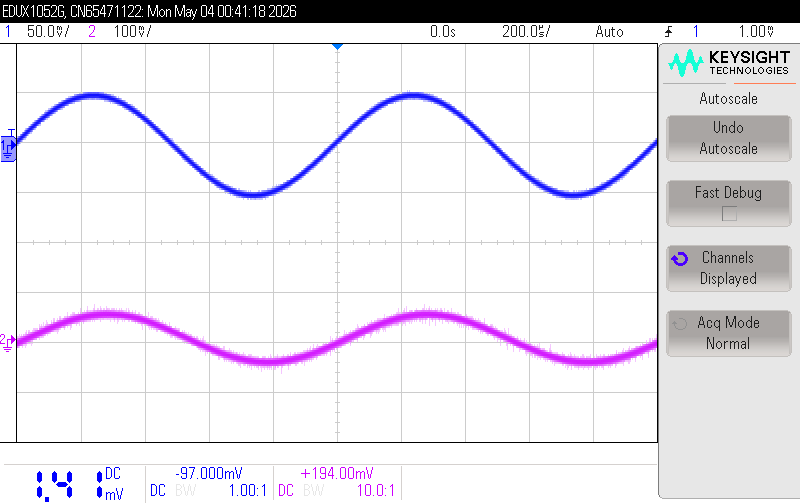
\includegraphics[width=\columnwidth]{images/lpf1k.png}
        \caption{Transient Response ($1\text{ kHz}$ Input).}
        \label{fig:lpf_1k}
    \end{subfigure}
    
    \vspace{0.3cm}
    \begin{subfigure}[b]{\columnwidth}
        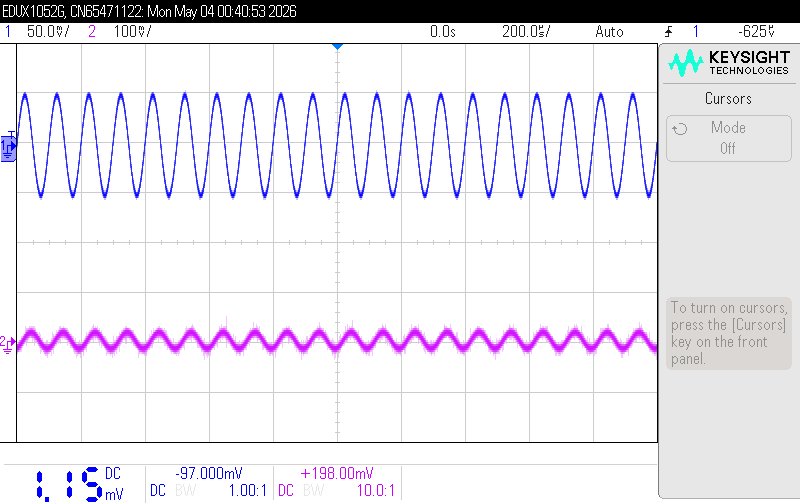
\includegraphics[width=\columnwidth]{images/lpf10k.png}
        \caption{Transient Response ($10\text{ kHz}$ Input).}
        \label{fig:lpf_10k}
    \end{subfigure}
    
    \vspace{0.3cm}
    \begin{subfigure}[b]{\columnwidth}
        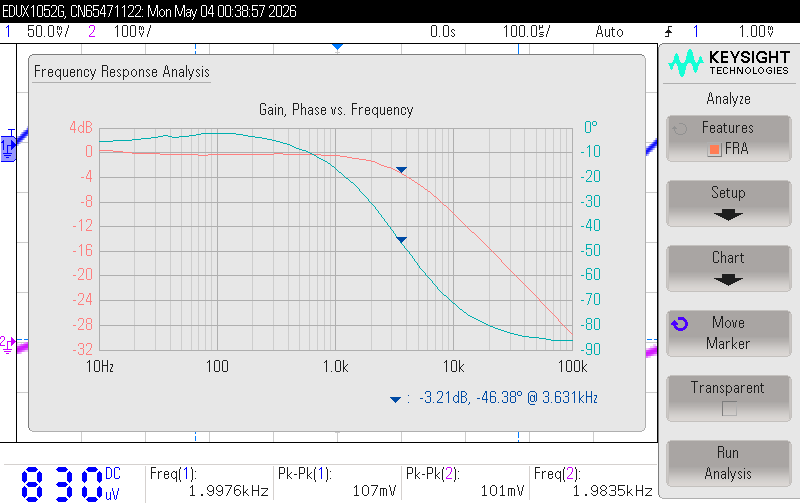
\includegraphics[width=\columnwidth]{images/frequency-response-2.png}
        \caption{AC Frequency Response (Bode Plot).}
        \label{fig:lpf_bode}
    \end{subfigure}
    \caption{Hardware Measurements for the Low-Pass Filter.}
    \label{fig:lpf_hardware}
\end{figure}

The hardware results correlate closely with the theoretical calculations. As shown in the transient measurements, the filter successfully passes the lower frequency signals (e.g., $1\text{ kHz}$) with minimal attenuation, while significantly attenuating higher frequency signals (e.g., $10\text{ kHz}$), confirming the calculated $-3\text{ dB}$ cut-off frequency near $3.39\text{ kHz}$. The Bode plot further validates the expected $-20\text{ dB/decade}$ roll-off characteristic of the first-order RC filter.

\subsection{Mixer and LPF Integration \& Iterative Optimization (Q4(e))}
Connecting the NMOS mixer output directly to the Low-Pass Filter represents a critical integration step in the receiver chain. During testing, an iterative design approach was taken to optimize the extraction of the $5\text{ kHz}$ IF signal while sufficiently suppressing high-frequency switching noise.

\subsubsection{Iteration 1: Single-Stage LPF}
Initially, a single-stage RC Low-Pass Filter was implemented using a $4.7\text{ k}\Omega$ resistor and a $10\text{ nF}$ capacitor. While this configuration provided an appropriate $-3\text{ dB}$ cut-off frequency ($3.39\text{ kHz}$), a single RC pole only offers a $-20\text{ dB/decade}$ roll-off. As shown in the measurement below, this relatively gentle roll-off was insufficient to completely eliminate the harsh switching transients and high-frequency sum components generated by the mixer, resulting in a noisy IF envelope.

\begin{figure}[htbp]
    \centering
    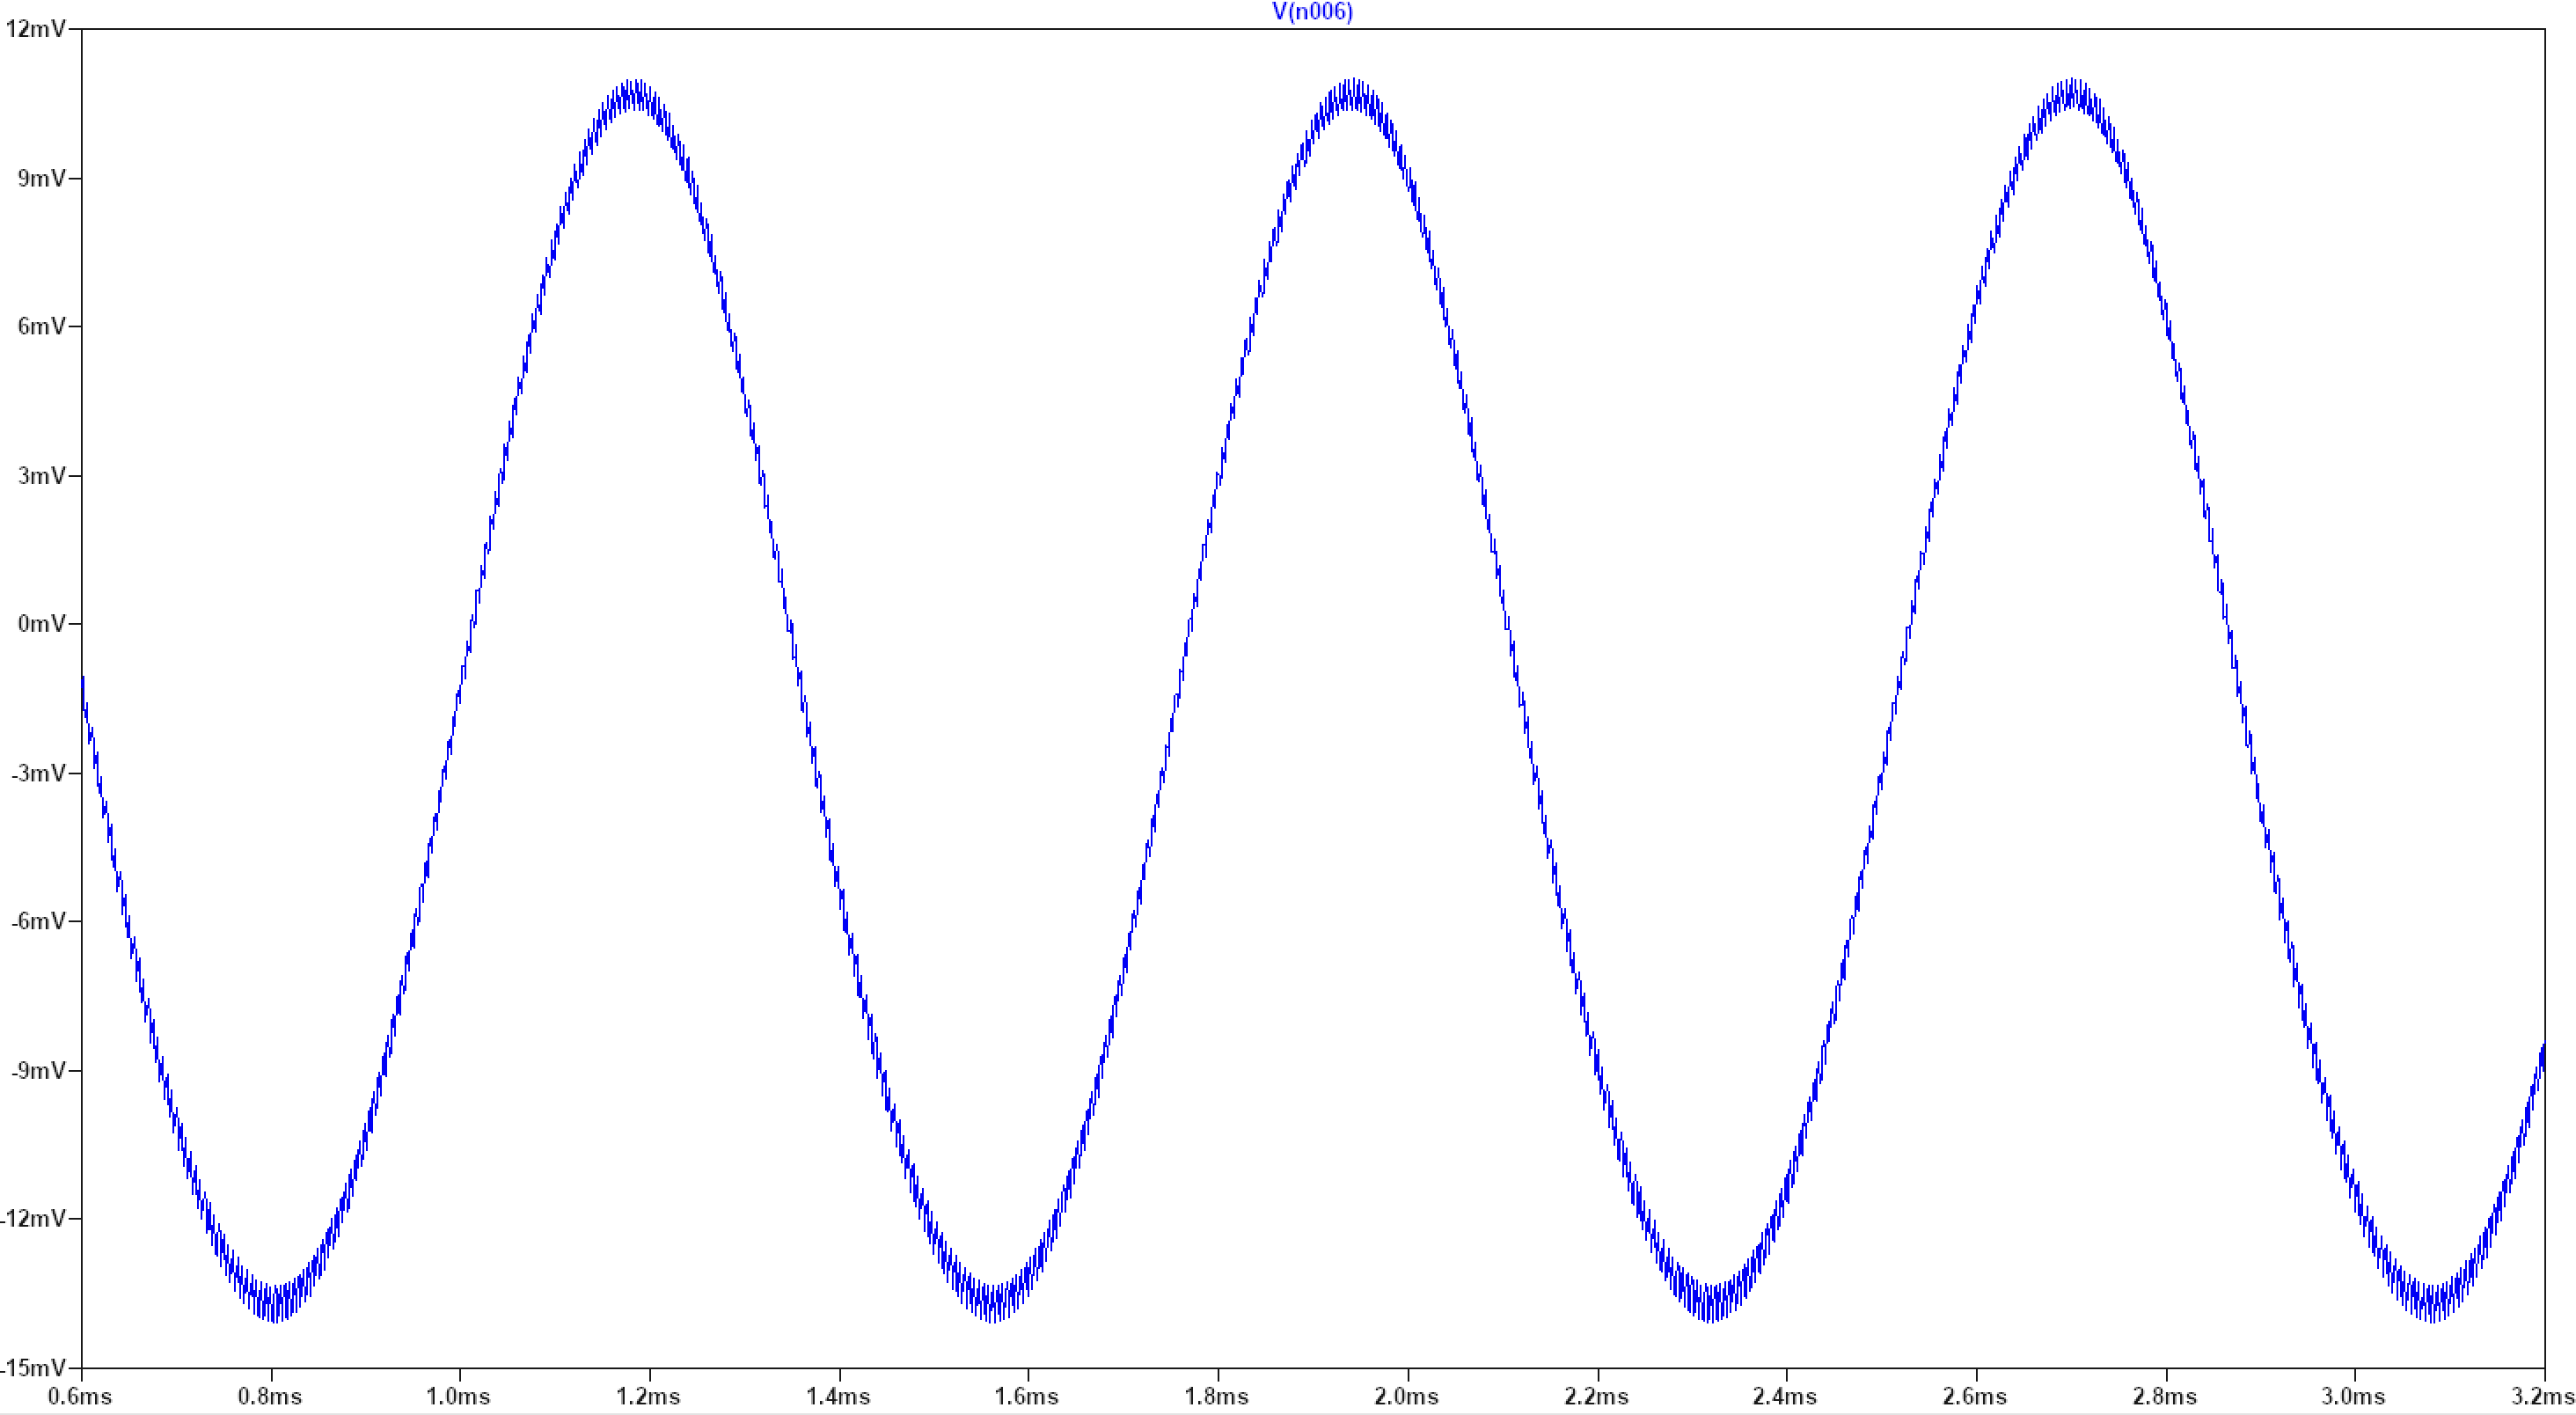
\includegraphics[width=\columnwidth]{images/mixer+1lpf.png}
    \caption{Mixer Output with a Single-Stage LPF (Visible High-Frequency Noise).}
    \label{fig:mixer_1lpf}
\end{figure}

\subsubsection{Iteration 2: Two-Stage Cascaded LPF}
To achieve better out-of-band rejection, the design was upgraded to a two-stage cascaded RC Low-Pass Filter. Each stage was constructed using a $2.2\text{ k}\Omega$ resistor and a $10\text{ nF}$ capacitor. 

For a single stage with these components, the nominal cut-off is:
$$f_{c, stage} = \frac{1}{2\pi \times 2200 \times (10 \times 10^{-9})} \approx 7.23\text{ kHz}$$
However, when two identical RC stages are cascaded, the overall $-3\text{ dB}$ cut-off frequency shifts downward. The cascaded $-3\text{ dB}$ frequency can be approximated by:
$$f_{c, cascaded} \approx f_{c, stage} \times \sqrt{\sqrt{2} - 1} \approx 7.23\text{ kHz} \times 0.6436 \approx 4.65\text{ kHz}$$

This dual-stage configuration places the combined cut-off right near the target $5\text{ kHz}$ IF signal. More importantly, it provides a steeper $-40\text{ dB/decade}$ attenuation beyond the cut-off frequency. As seen in the resulting measurement, this steeper roll-off successfully smoothed out the switching transients, yielding a much cleaner, high-quality IF output.

\begin{figure}[htbp]
    \centering
    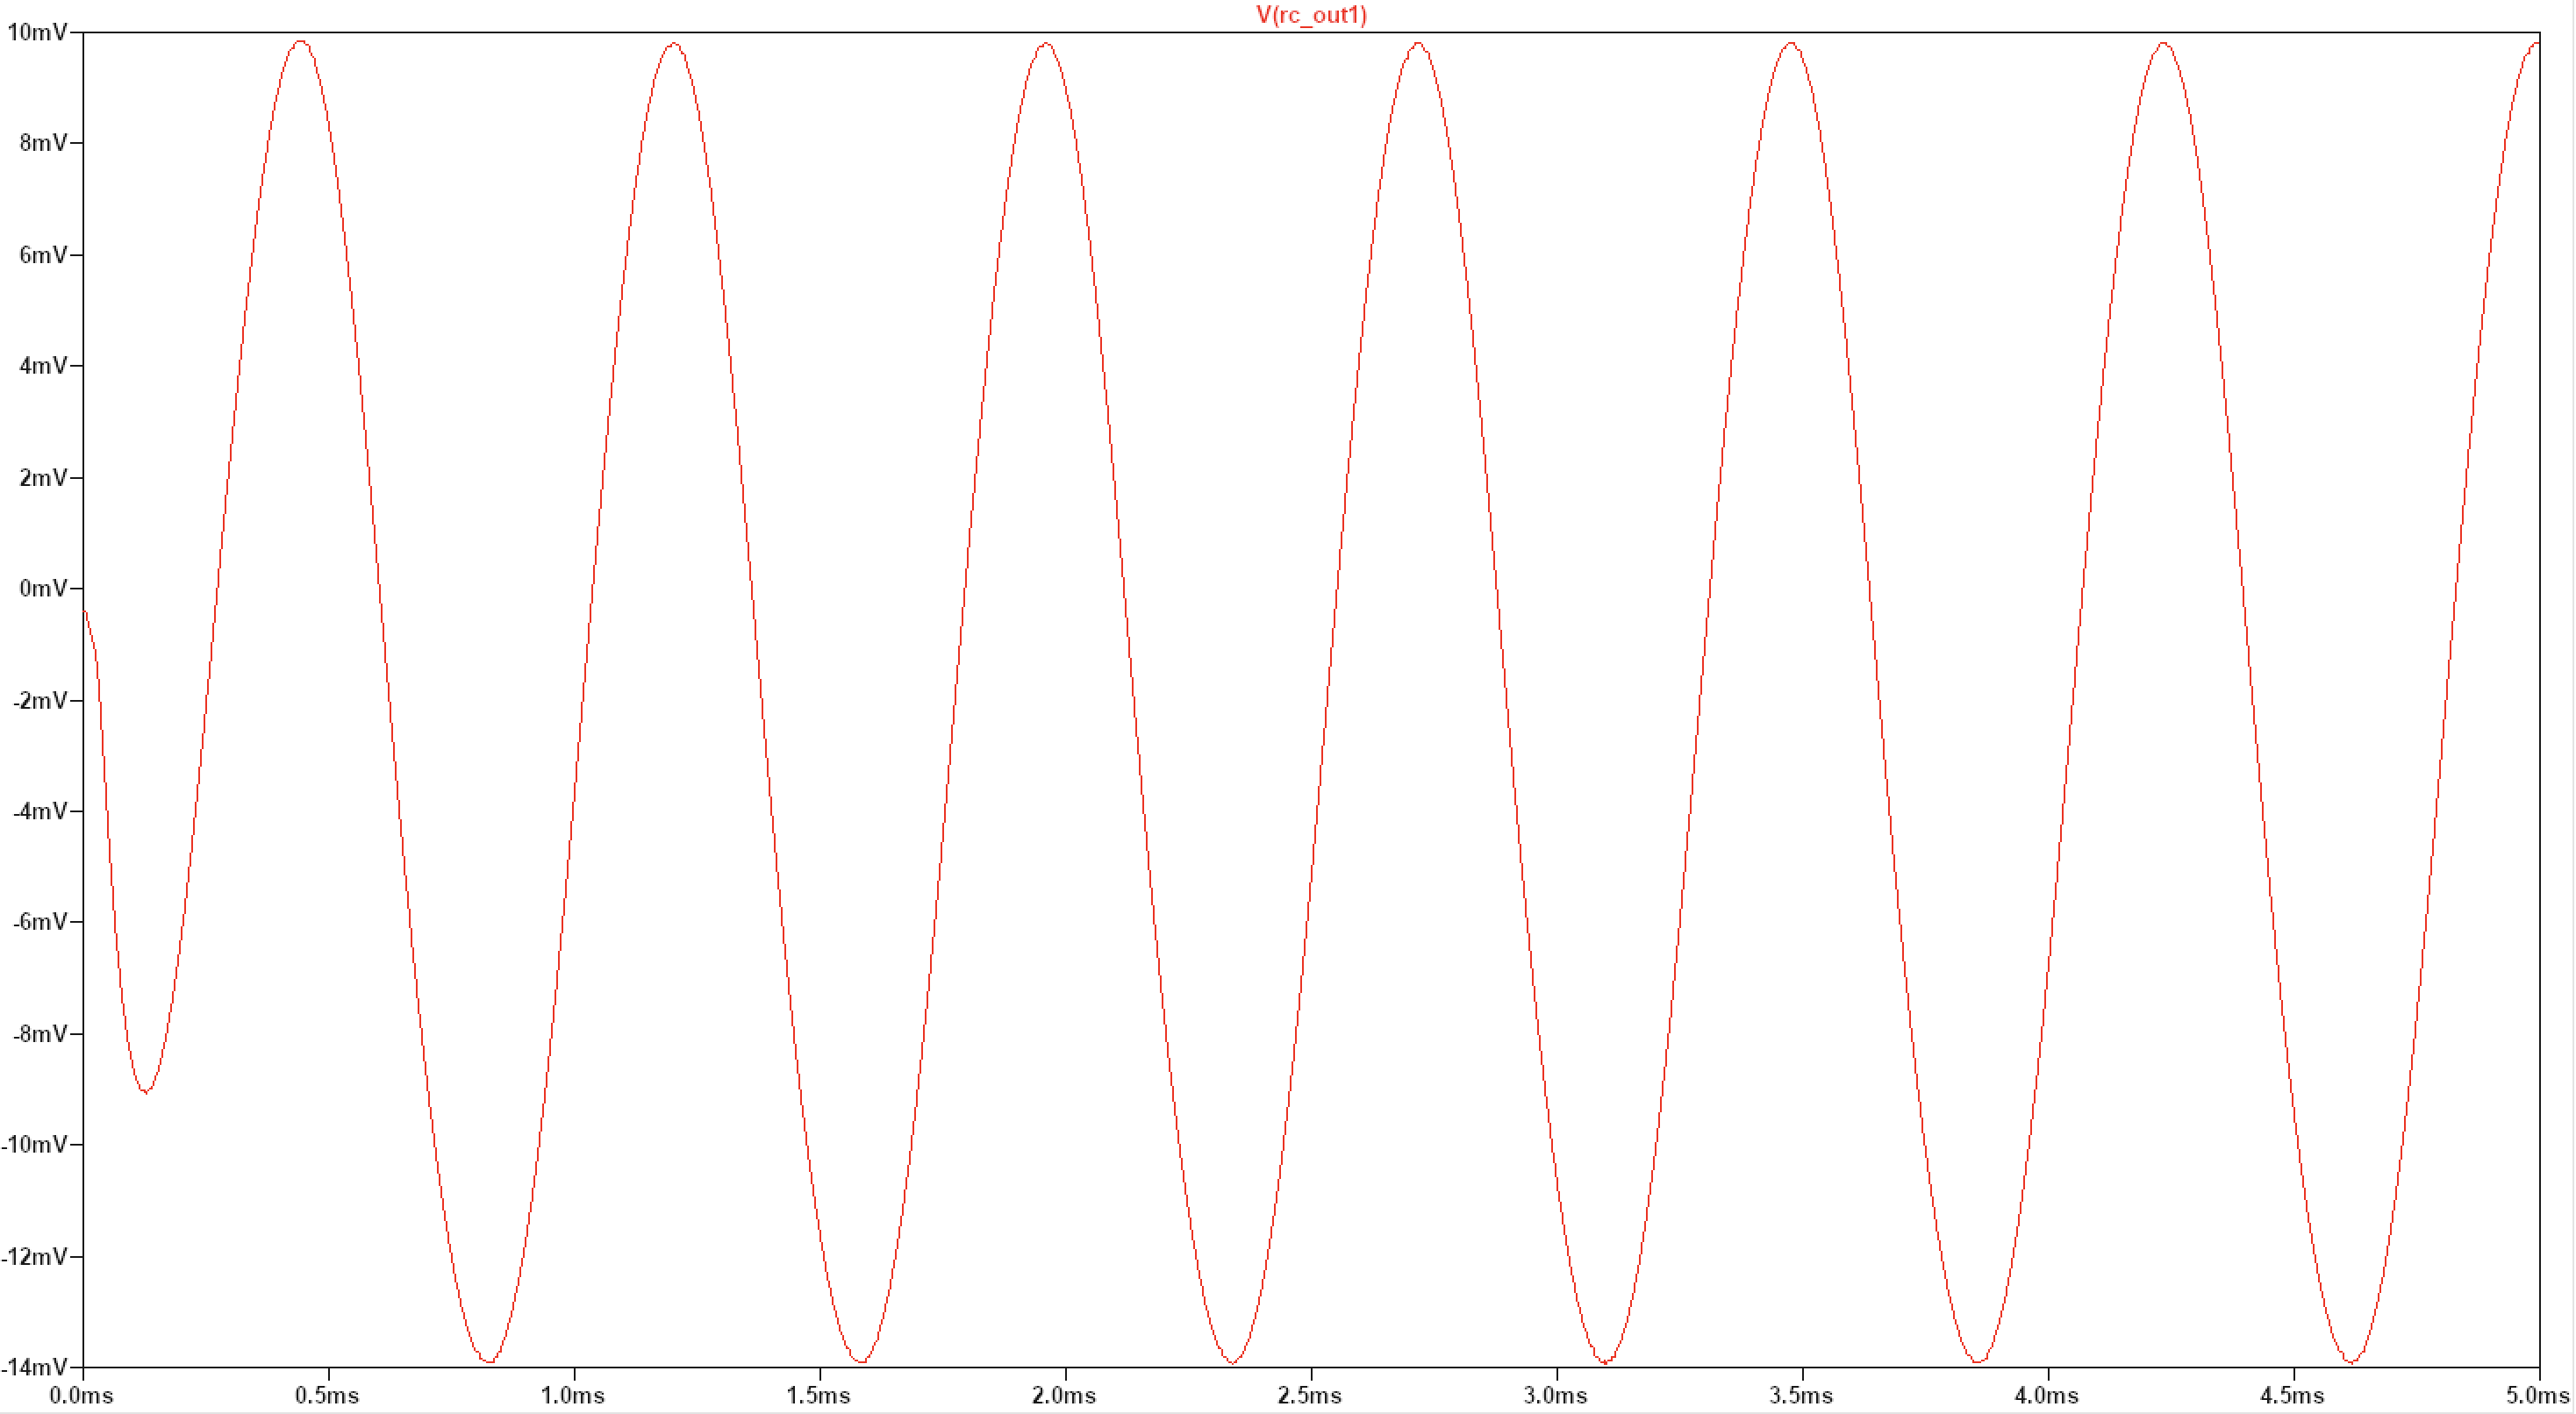
\includegraphics[width=\columnwidth]{images/mixer+2lpf.png}
    \caption{Mixer Output with a Two-Stage Cascaded LPF (Clean IF Envelope).}
    \label{fig:mixer_2lpf}
\end{figure}

\subsubsection{Hardware Measurement Verification}
To verify the performance of the final two-stage cascaded LPF design in the laboratory, the physical circuit was constructed and connected to the NMOS mixer output. The resulting downconverted signals were captured using a Digital Storage Oscilloscope (DSO).

\begin{figure}[htbp]
    \centering
    \begin{subfigure}[b]{\columnwidth}
        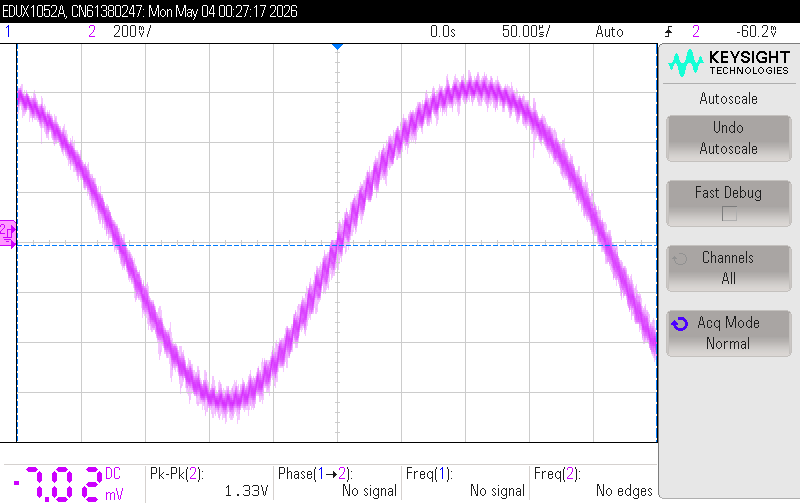
\includegraphics[width=\columnwidth]{images/low-pass-output.png}
        \caption{Hardware Measurement: Mixer + Cascaded LPF Output 1.}
        \label{fig:lpf_dso_1}
    \end{subfigure}
    
    \vspace{0.3cm}
    \begin{subfigure}[b]{\columnwidth}
        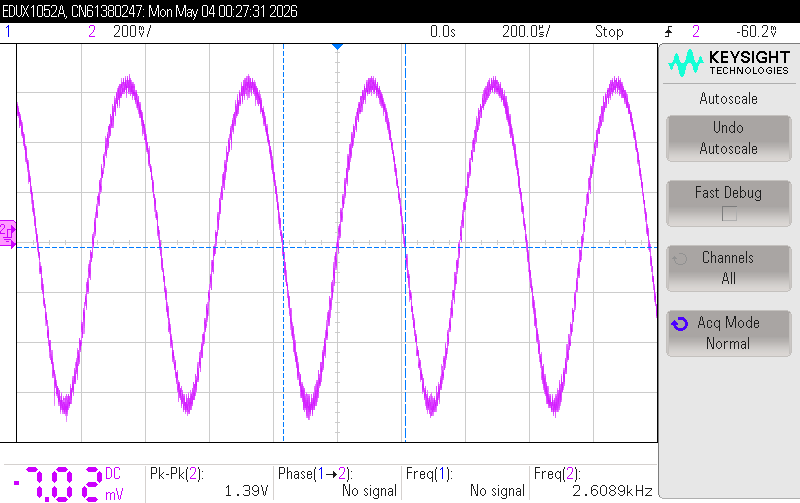
\includegraphics[width=\columnwidth]{images/low-pass-output-img2.png}
        \caption{Hardware Measurement: Mixer + Cascaded LPF Output 2.}
        \label{fig:lpf_dso_2}
    \end{subfigure}
    \caption{DSO Measurements of the Integrated Mixer and LPF Circuit.}
    \label{fig:mixer_lpf_dso}
\end{figure}

The DSO measurements confirm that the physical implementation successfully extracts the low-frequency IF envelope while effectively attenuating the high-frequency carrier and switching noise, perfectly validating the theoretical and simulated designs.
\section{CE BJT Amplifier Design}
Because the two-stage cascaded LPF introduces significant attenuation, the amplitude of the $5\text{ kHz}$ IF signal drops to approximately $8\text{ mV}$. To restore the signal and boost it to the specified target of $>450\text{ mV}$, a Common Emitter (CE) BJT amplifier stage was designed and integrated.

\subsection{Design Constraints \& THD Optimization}
A standard CE amplifier with a fully bypassed emitter provides the maximum possible voltage gain. However, relying solely on the internal emitter resistance ($r_e$) often leads to high Total Harmonic Distortion (THD) when handling larger signal swings. To mitigate this and linearize the amplifier, a small unbypassed emitter resistor ($R_{E1}$) was intentionally introduced (emitter degeneration).

\subsection{Mathematical Derivations}
The DC biasing network was designed to establish a quiescent emitter current of $I_E \approx 1.46\text{ mA}$. 
The internal dynamic emitter resistance ($r_e$) is calculated as:
\begin{equation}
    r_e = \frac{V_T}{I_E} \approx \frac{26\text{ mV}}{1.46\text{ mA}} \approx 17.8\ \Omega
\end{equation}

By selecting a collector resistor $R_C = 2\text{ k}\Omega$ and adding an unbypassed emitter resistor $R_{E1} = 15\ \Omega$, the AC voltage gain ($A_v$) becomes:
\begin{equation}
    A_v \approx \frac{R_C}{R_{E1} + r_e} = \frac{2000}{15 + 17.8} \approx 61
\end{equation}

With the cascaded LPF providing an $8\text{ mV}$ input to the amplifier, the expected final output voltage swing is:
\begin{equation}
    V_{out} = V_{in} \times A_v \approx 8\text{ mV} \times 61 \approx 488\text{ mV}
\end{equation}
This expected output comfortably satisfies the $>450\text{ mV}$ design requirement while drastically reducing the Total Harmonic Distortion (THD).

\subsection{Hardware Integration \& Verification}
The physical amplifier circuit was constructed and cascaded immediately following the two-stage LPF. 

\begin{figure}[htbp]
    \centering
    \begin{subfigure}[b]{\columnwidth}
        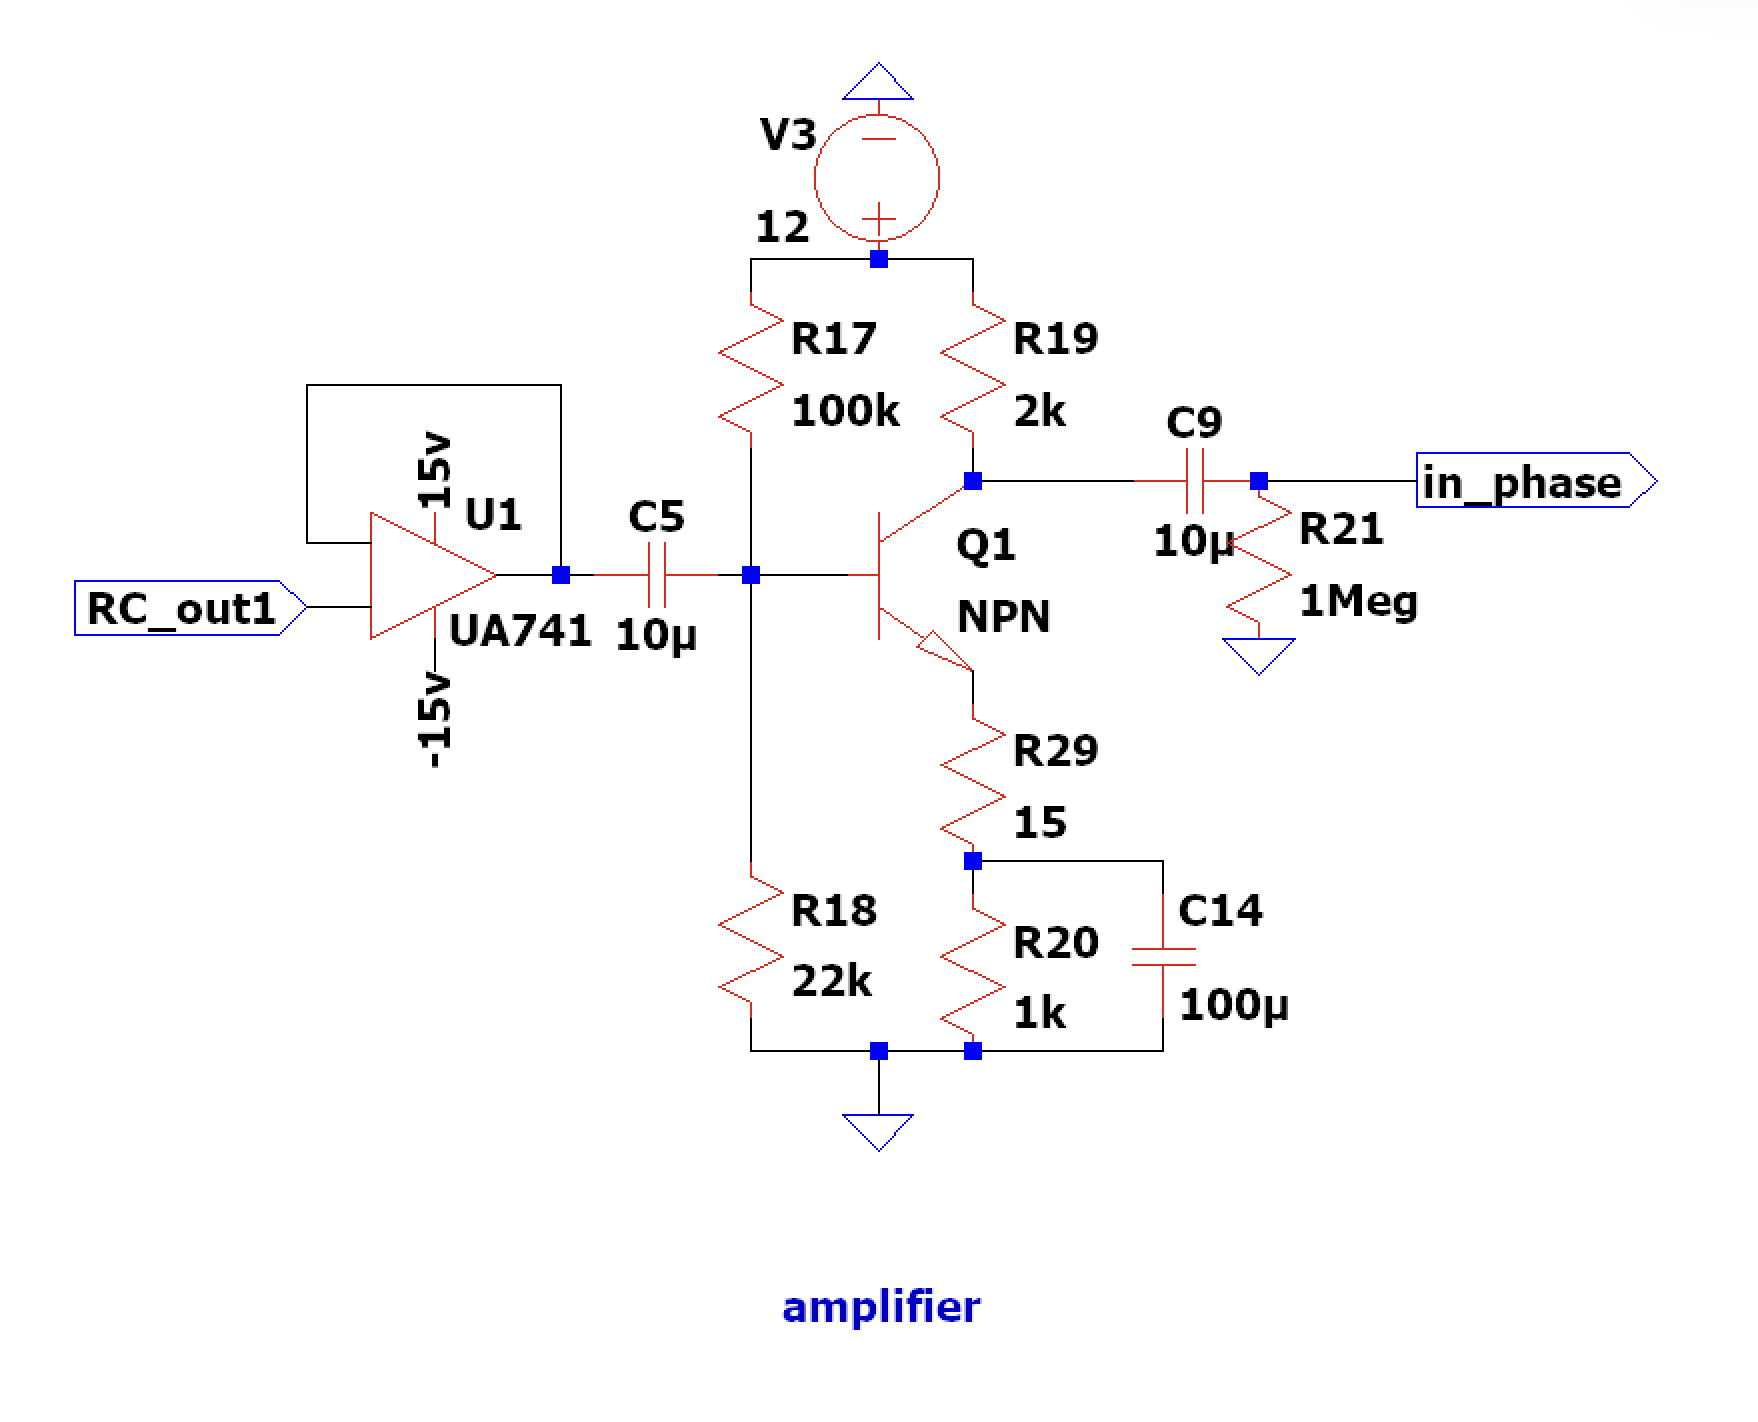
\includegraphics[width=\columnwidth]{images/amplifier.png}
        \caption{Hardware Realization of the CE BJT Amplifier.}
        \label{fig:amplifier_circ}
    \end{subfigure}
    
    \vspace{0.3cm}
    \begin{subfigure}[b]{\columnwidth}
        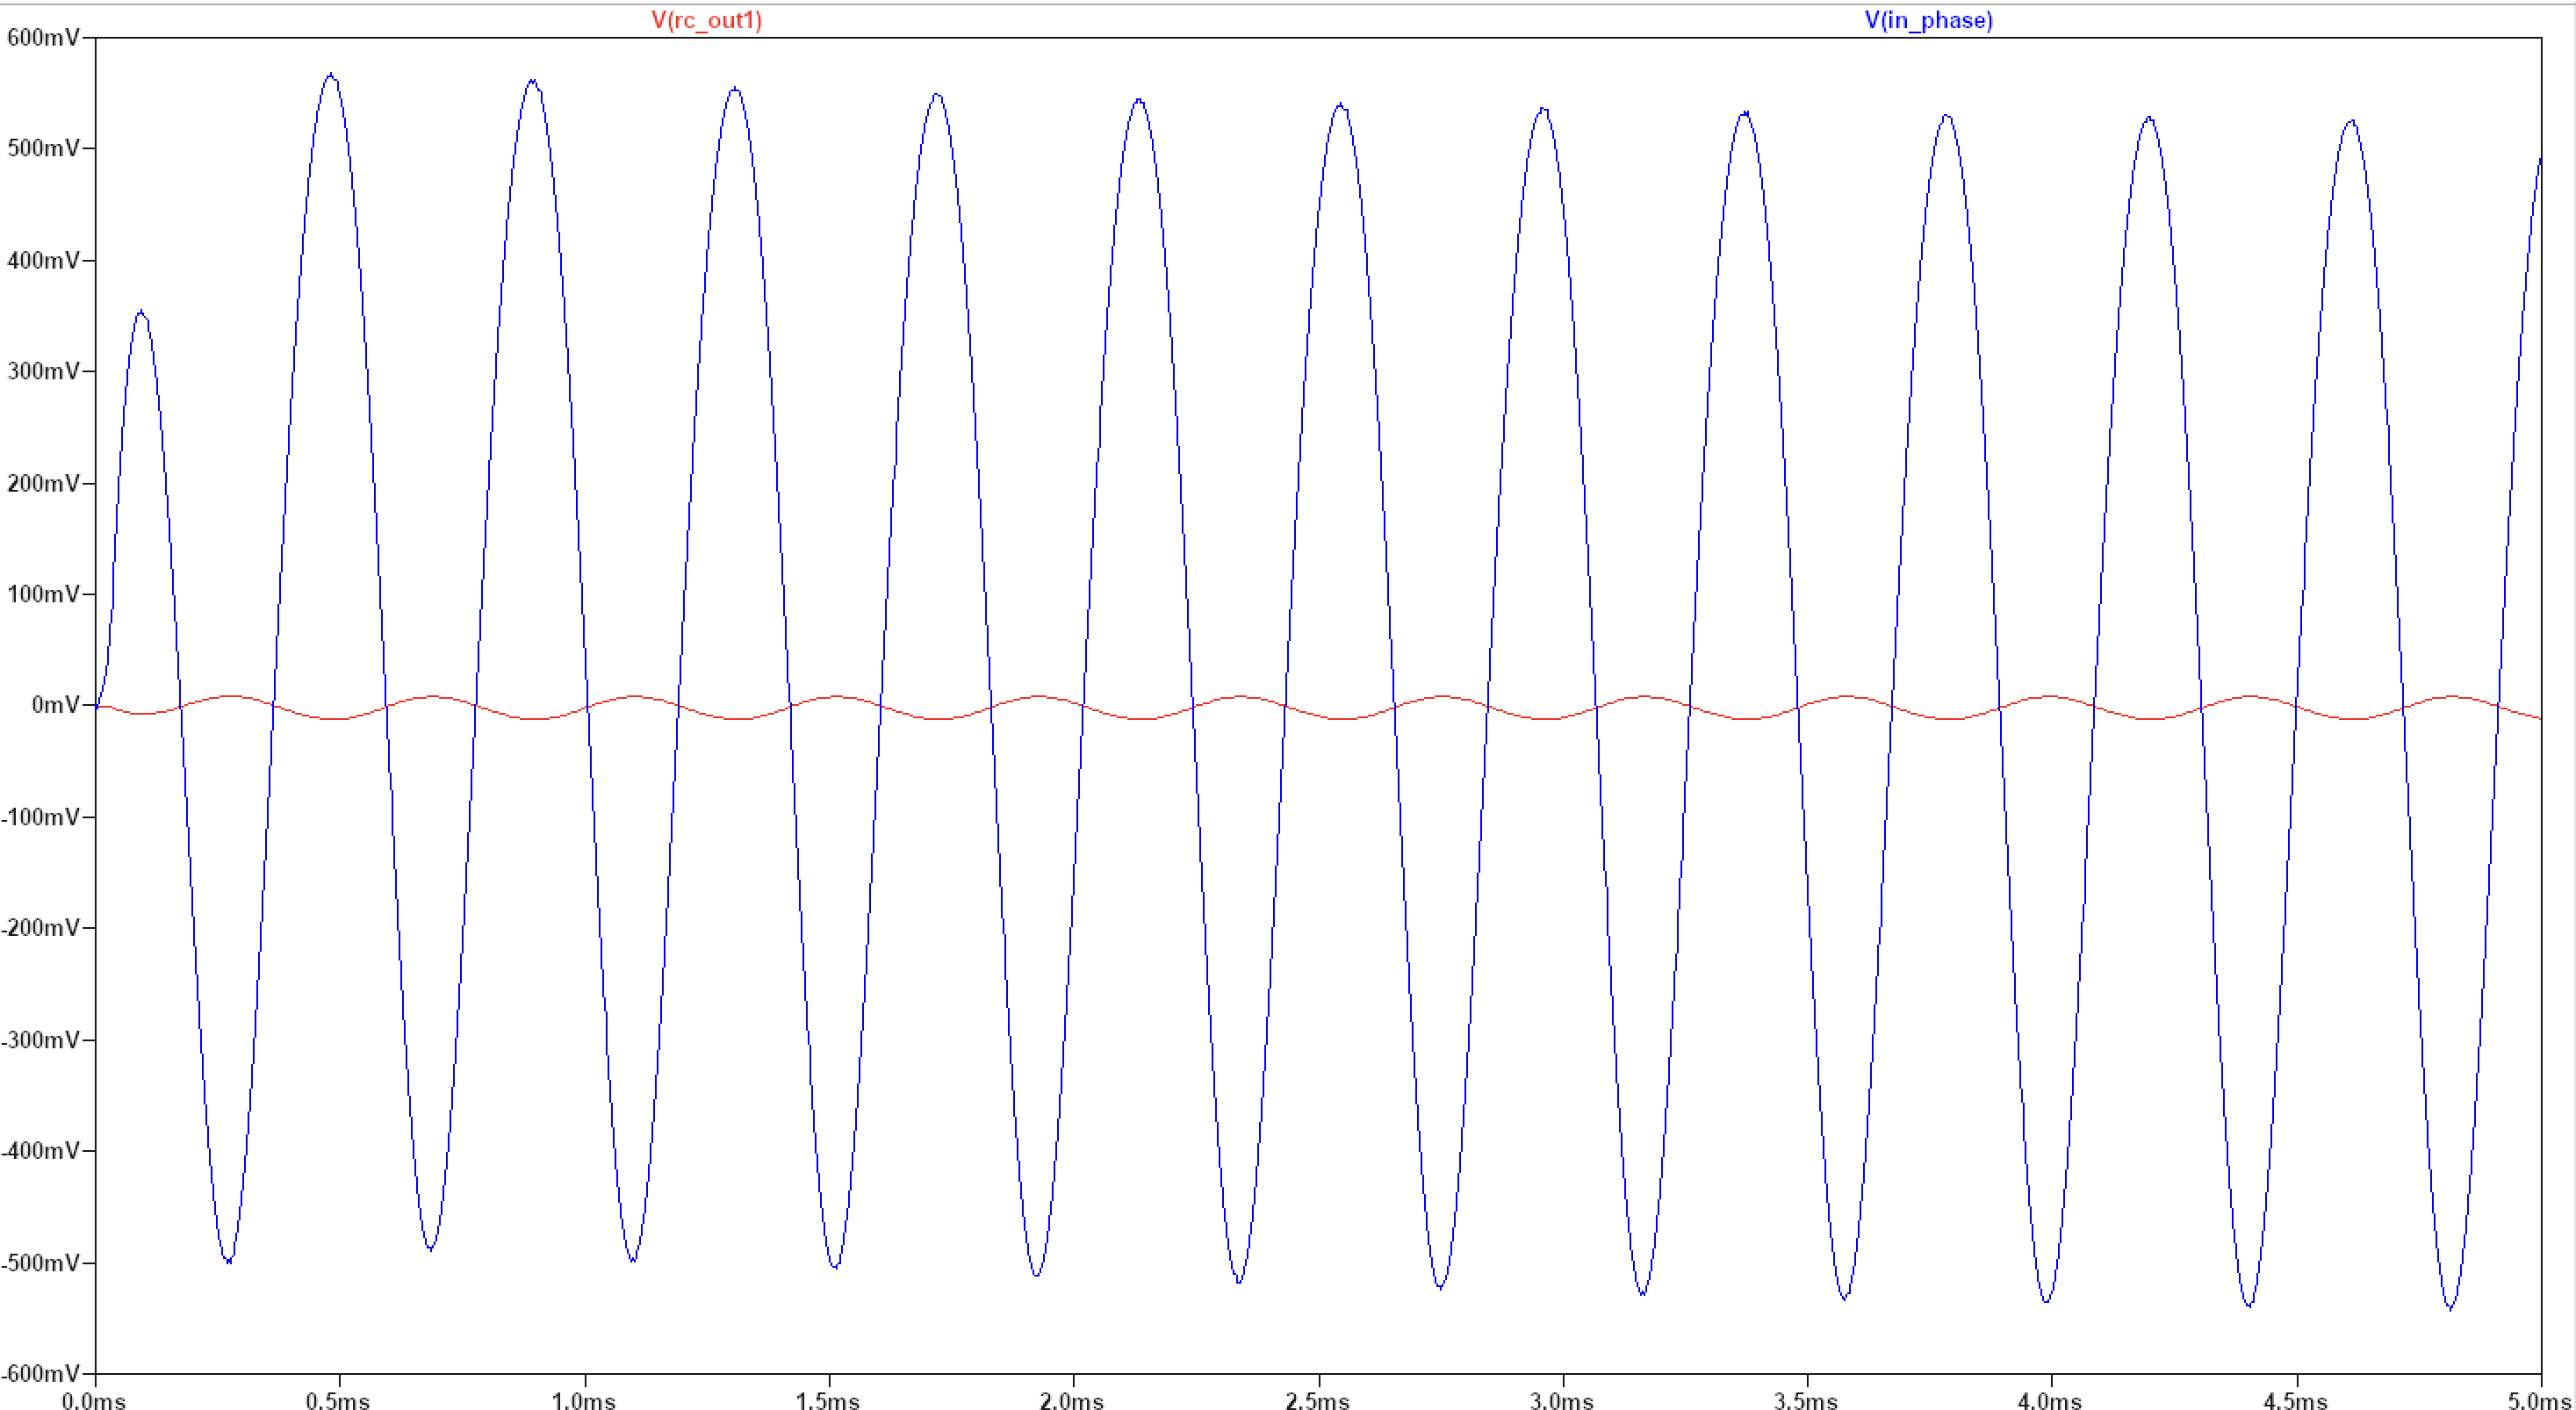
\includegraphics[width=\columnwidth]{images/LPF+amp.png}
        \caption{Integrated Output: Mixer + LPF + CE Amplifier.}
        \label{fig:lpf_amp_out}
    \end{subfigure}
    \caption{Final Amplifier Stage Implementation and Output.}
    \label{fig:amp_hardware}
\end{figure}

\section{Complete Circuit Prototype Design (Q5)}
The final system-level prototype seamlessly integrates the quadrature oscillator, two independent NMOS switch mixers, two cascaded RC low-pass filters, and two CE BJT amplifiers to yield the final downconverted In-Phase ($v_{IF\_FINAL\_I}$) and Quadrature-Phase ($v_{IF\_FINAL\_Q}$) signals.

\begin{figure}[htbp]
    \centering
    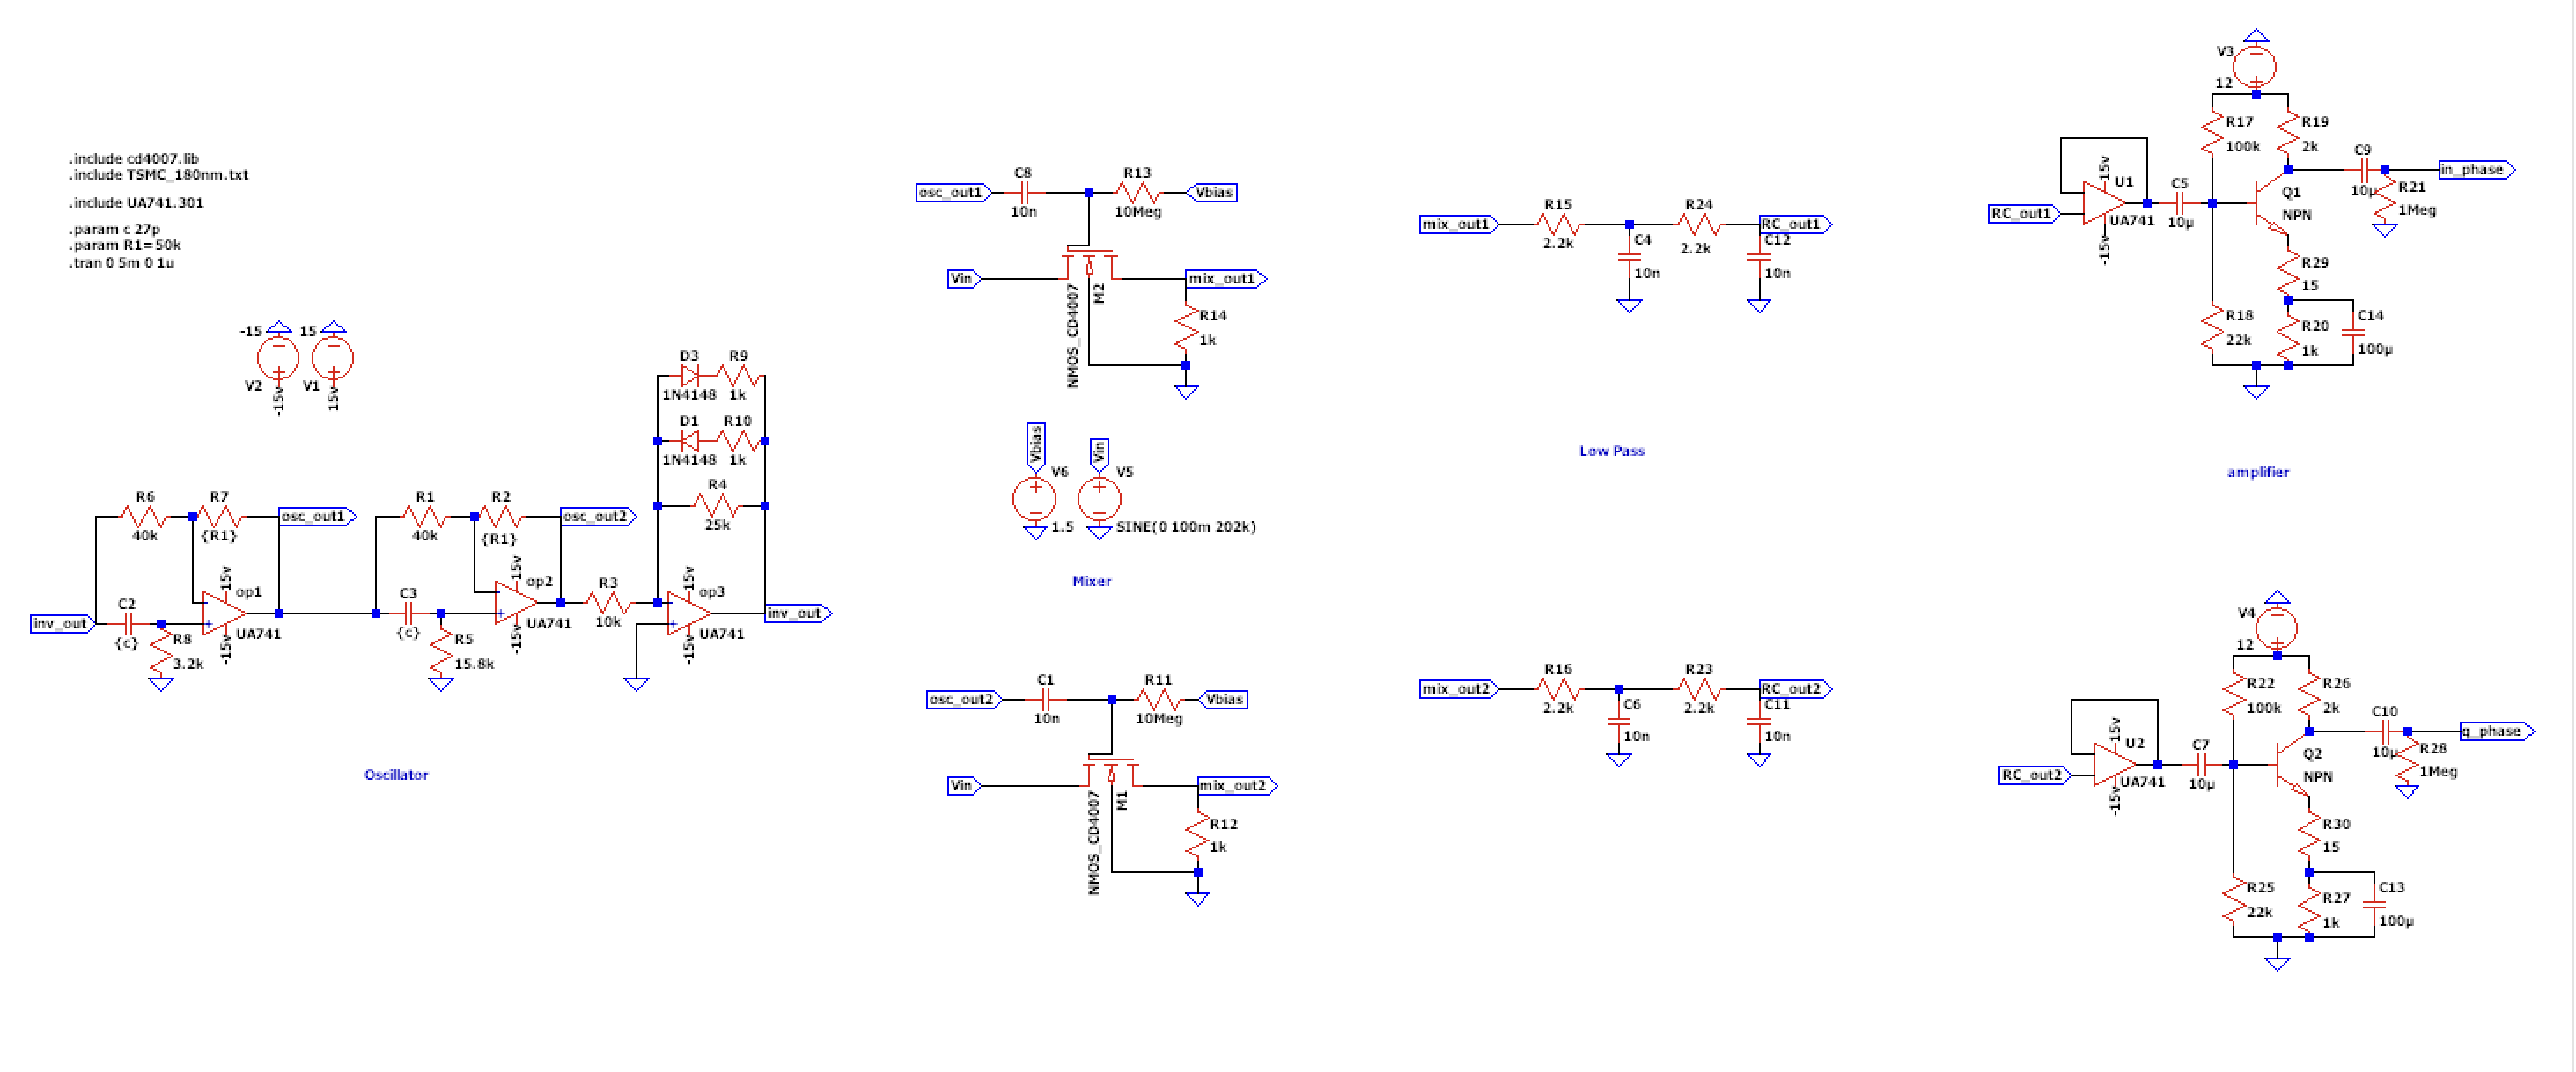
\includegraphics[width=\columnwidth]{images/5-final_circ.png}
    \caption{Complete Circuit Schematic showing the Oscillator, Mixers, Filters, and Amplifiers.}
    \label{fig:complete_schematic}
\end{figure}

\subsection{Transient and Frequency Simulation Results (Q5(a) \& Q5(b))}
To verify the theoretical foundation of the entire integrated system, transient simulations were executed. The primary goal was to confirm that the $90^\circ$ phase shift generated by the local quadrature oscillator accurately translates down to the $5\text{ kHz}$ Intermediate Frequency (IF) components.

\begin{figure}[htbp]
    \centering
    \begin{subfigure}[b]{\columnwidth}
        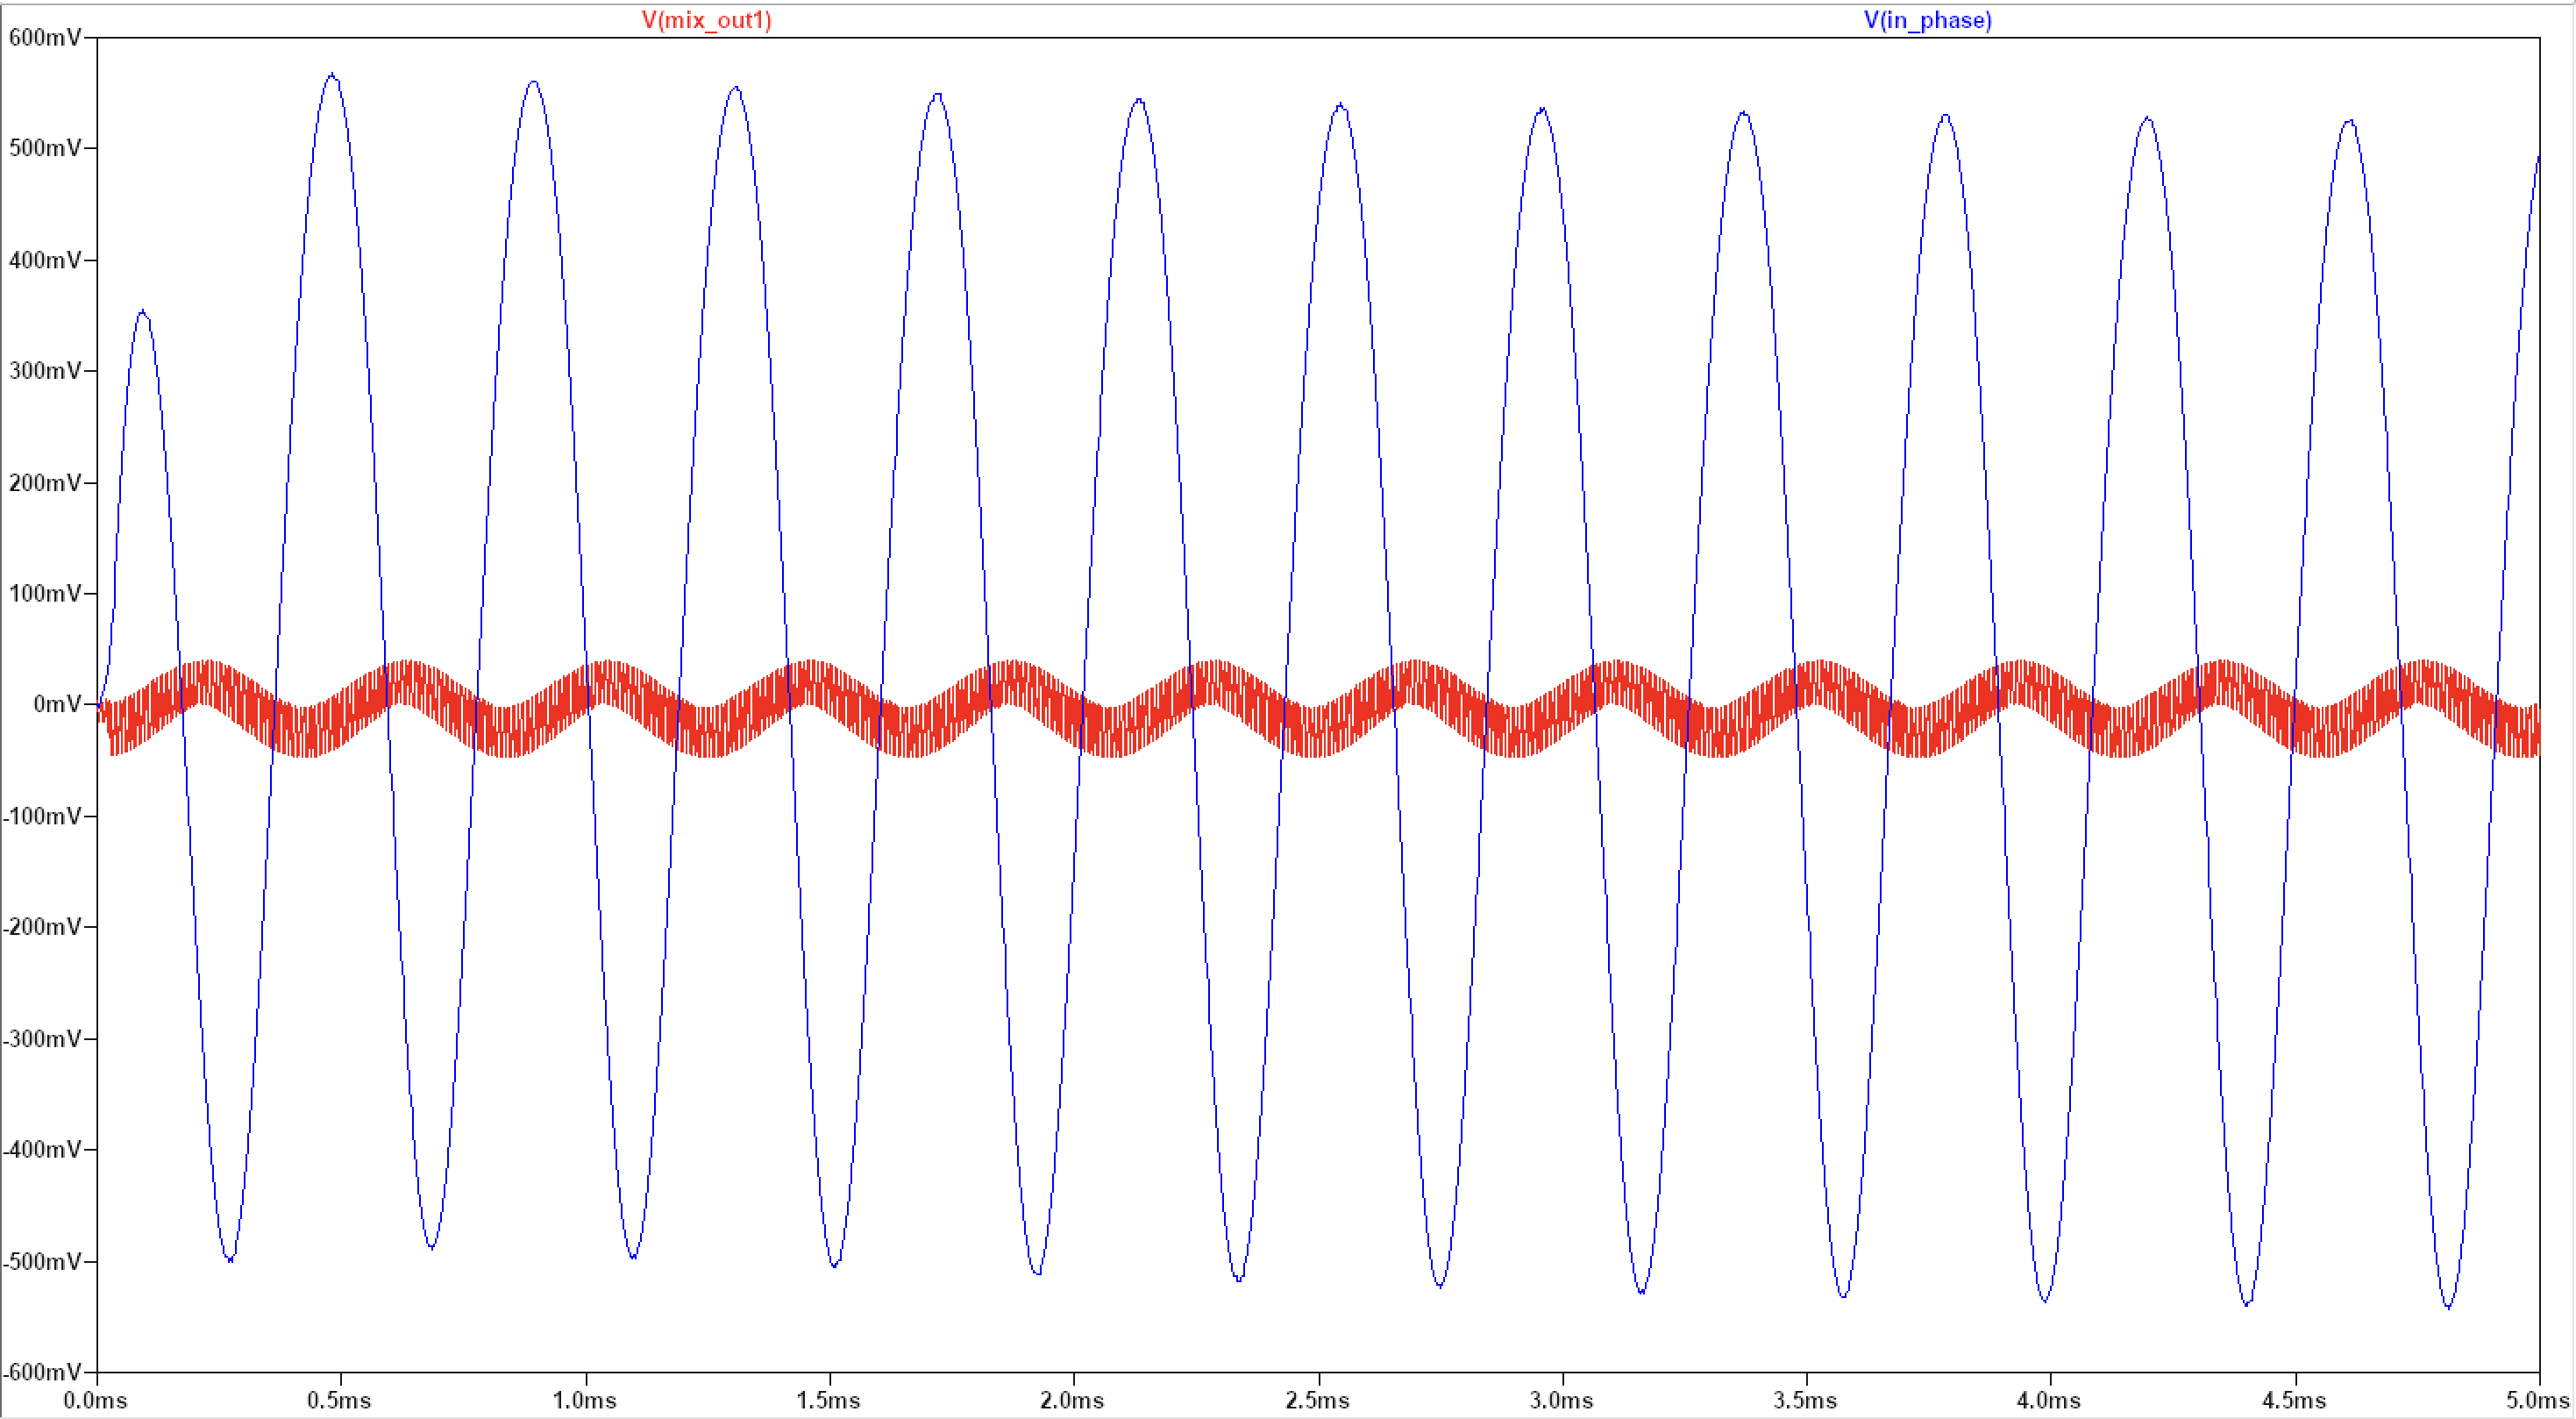
\includegraphics[width=\columnwidth]{images/5-If-If-final.png}
        \caption{Transient Simulation of the Final I and Q IF Signals.}
        \label{fig:sim_transient_iq}
    \end{subfigure}
    
    \vspace{0.3cm}
    \begin{subfigure}[b]{\columnwidth}
        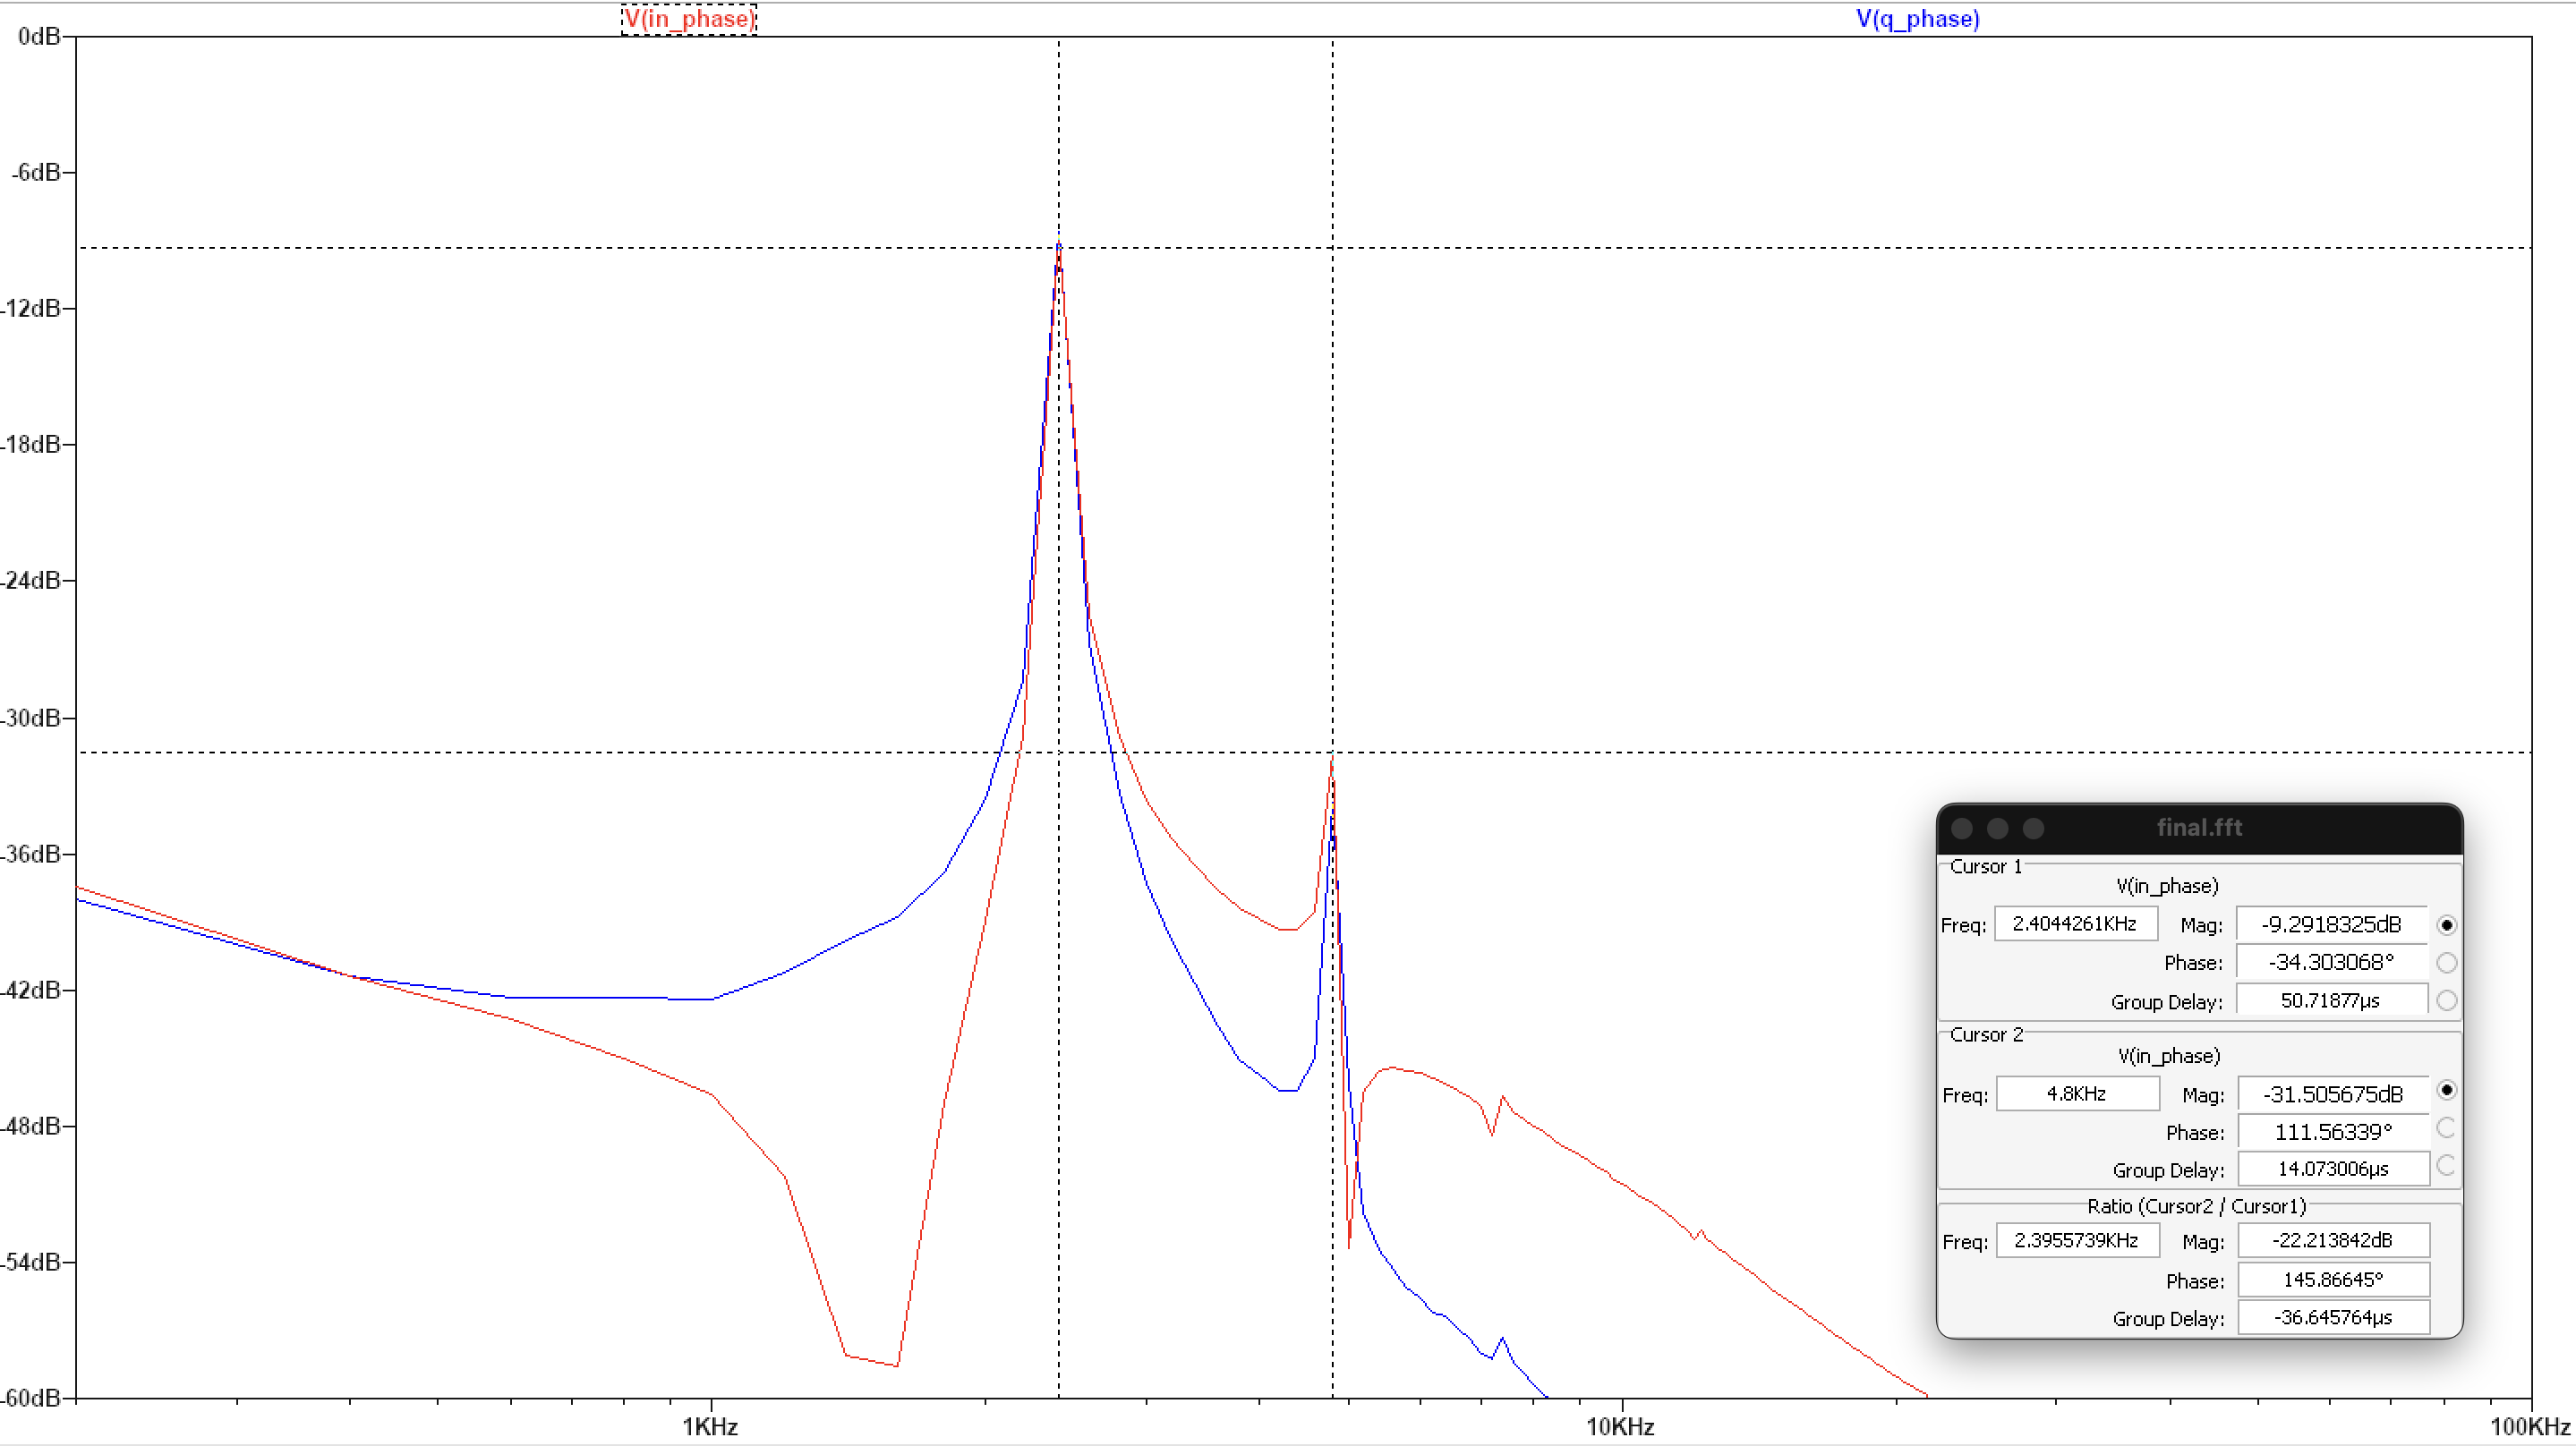
\includegraphics[width=\columnwidth]{images/5-iq-fft.png}
        \caption{FFT Spectrum of the Final I and Q IF Signals.}
        \label{fig:sim_fft_iq}
    \end{subfigure}
    \caption{System Simulation Results demonstrating $90^\circ$ Phase Shift and $5\text{ kHz}$ IF.}
    \label{fig:sim_final_results}
\end{figure}

The transient waveforms (Fig. \ref{fig:sim_transient_iq}) clearly display the final amplified IF signals. As theoretically predicted, the $90^\circ$ phase difference established by the high-frequency $170\text{ kHz}$ quadrature oscillator is perfectly preserved during the non-linear downconversion process, resulting in a low-frequency $5\text{ kHz}$ sine and cosine pair. The FFT plot (Fig. \ref{fig:sim_fft_iq}) confirms the spectral purity of these signals, showing dominant, identical peaks strictly at $5\text{ kHz}$ with minimal spurious harmonics.

\subsection{Hardware Realization and Measurements (Q5(c) \& Q5(d))}
The entire theoretical topology was physically realized in the laboratory. Probing the multi-stage system confirmed its real-world viability.

\begin{figure}[htbp]
    \centering
    \begin{subfigure}[b]{\columnwidth}
        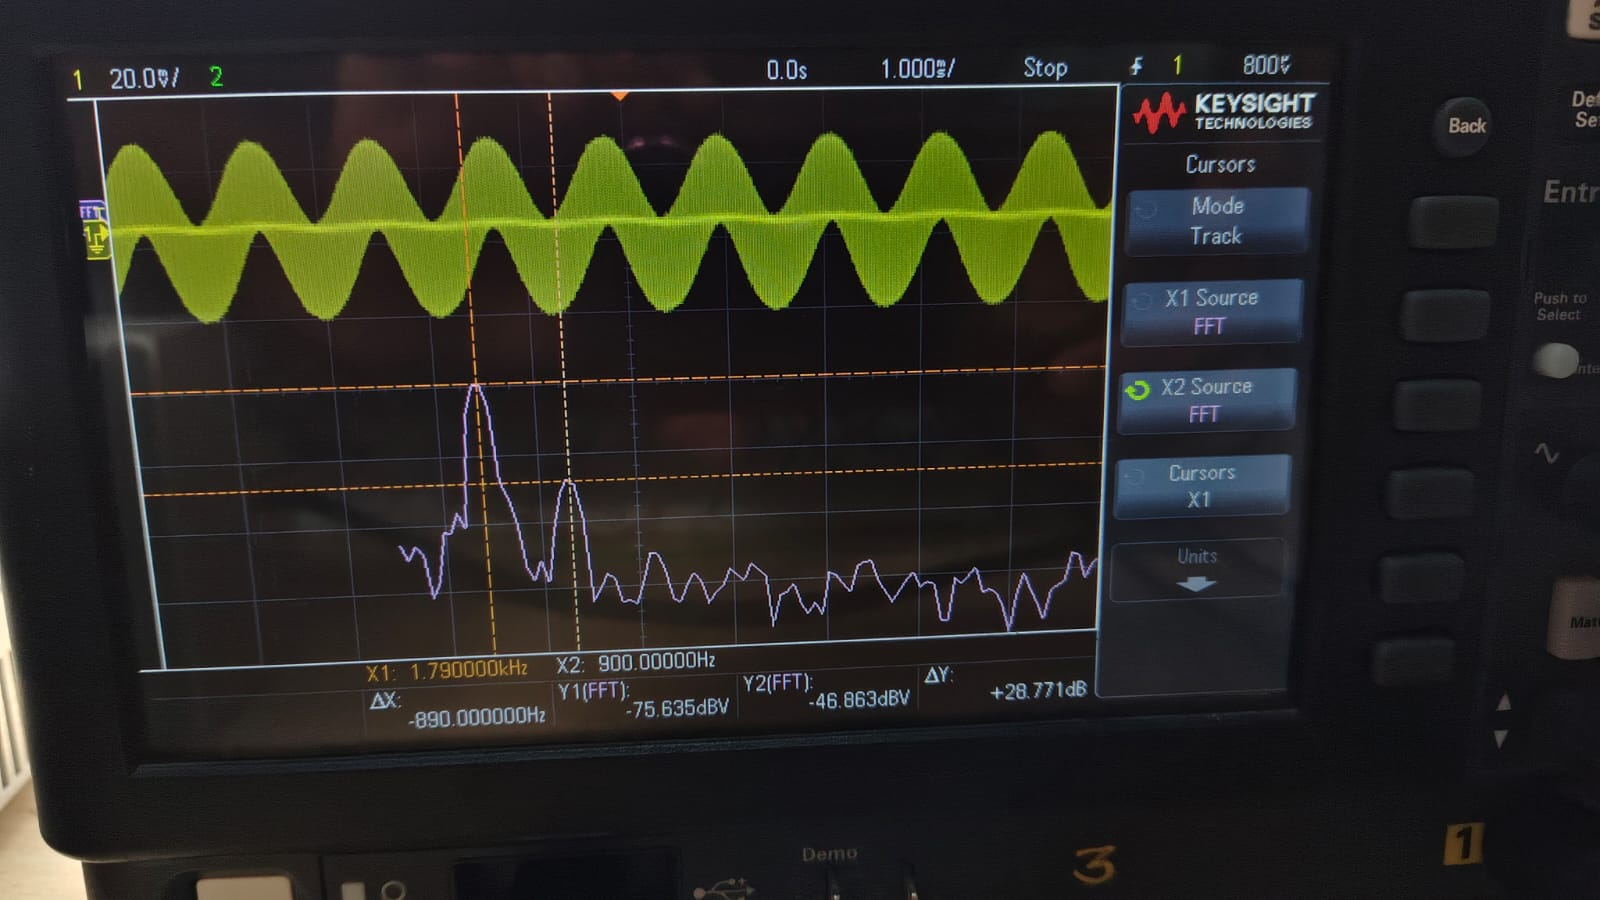
\includegraphics[width=\columnwidth]{images/5-Vif.jpeg}
        \caption{DSO Measurement: Single IF Output.}
        \label{fig:dso_vif}
    \end{subfigure}
    
    \vspace{0.3cm}
    \begin{subfigure}[b]{\columnwidth}
        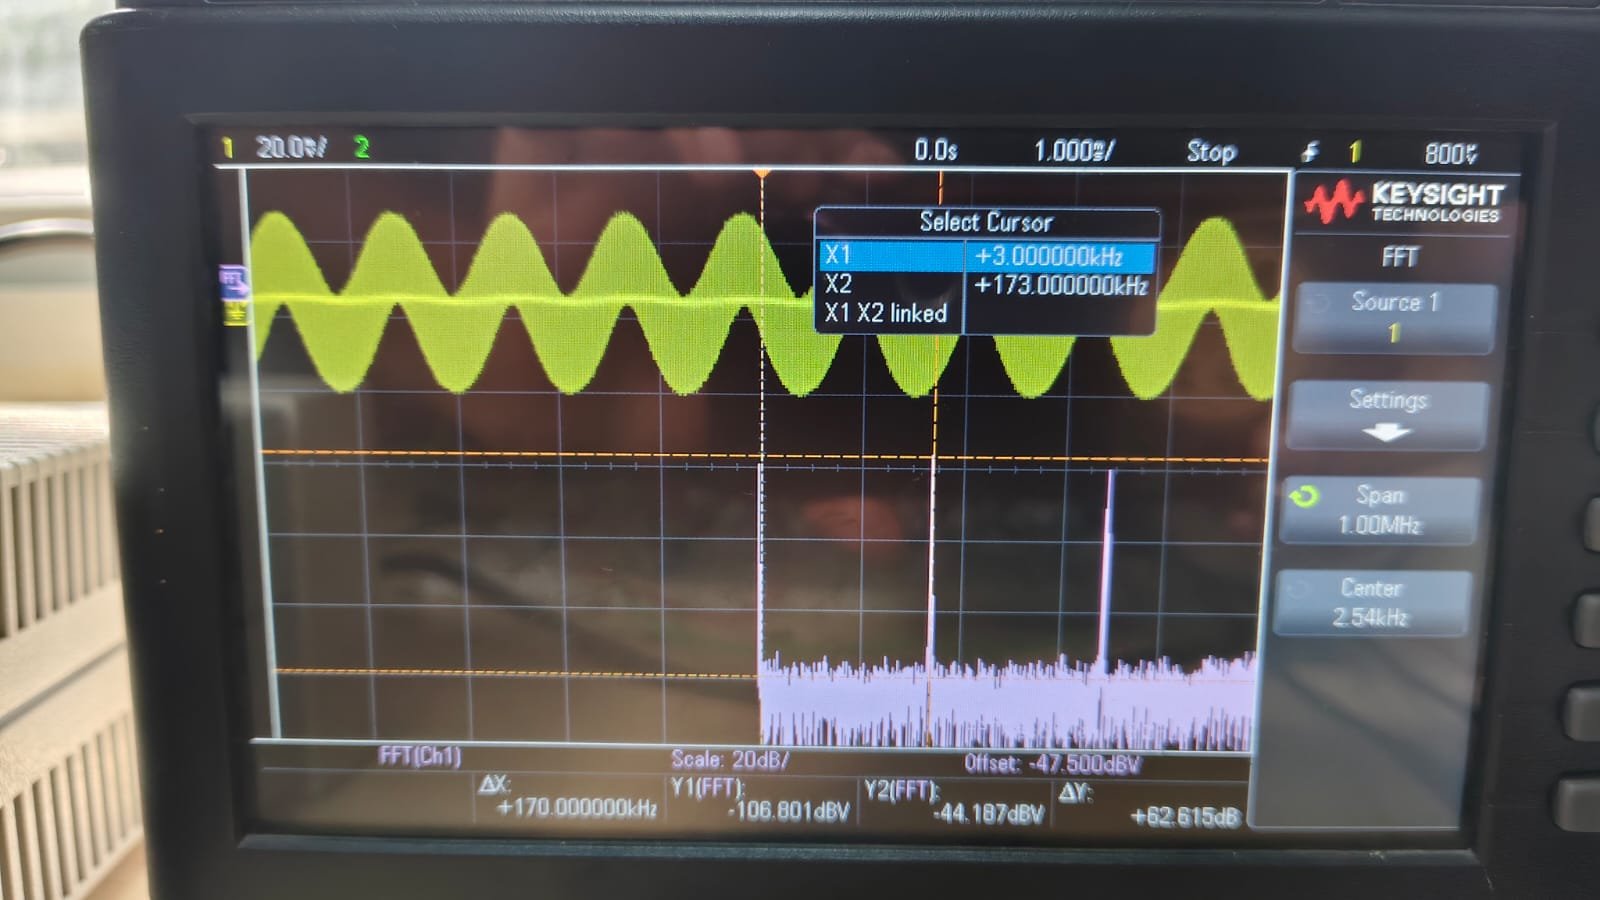
\includegraphics[width=\columnwidth]{images/5-vif+170.jpeg}
        \caption{DSO Measurement: IF Output with $170\text{ kHz}$ RF Input Envelope.}
        \label{fig:dso_vif_rf}
    \end{subfigure}
    \caption{Hardware Measurements of the Mixer and LPF Operations.}
    \label{fig:dso_mixer_operations}
\end{figure}

\begin{figure}[htbp]
    \centering
    \begin{subfigure}[b]{\columnwidth}
        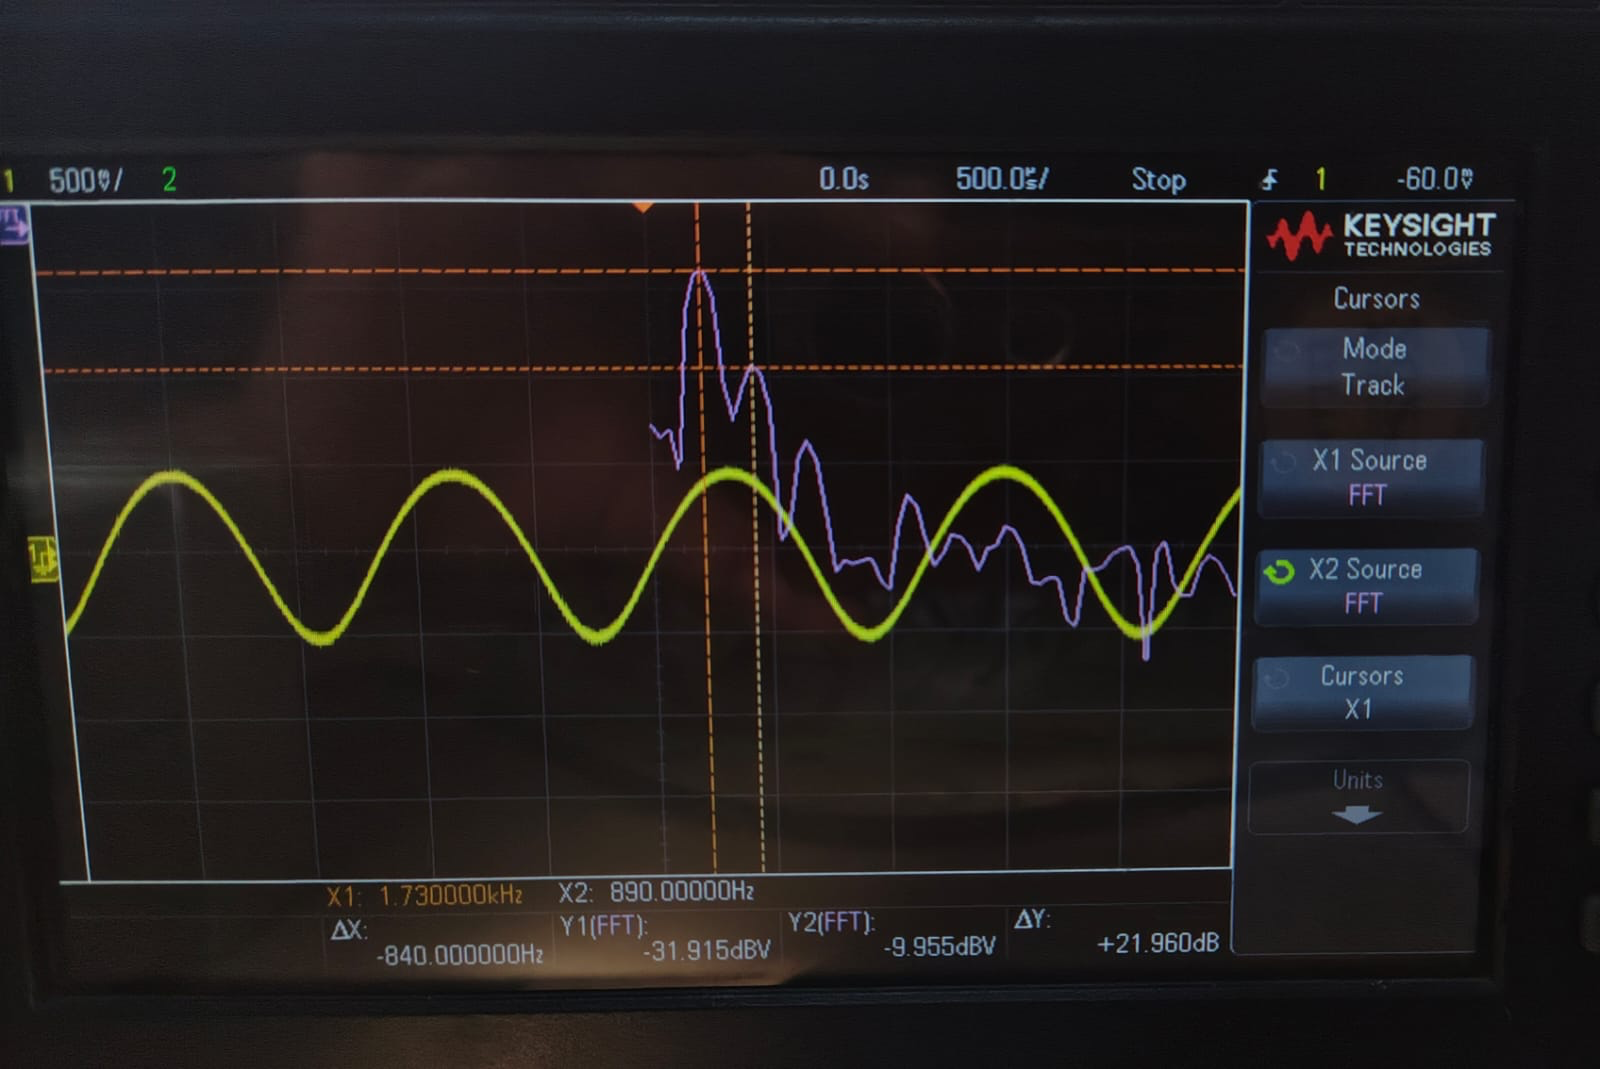
\includegraphics[width=\columnwidth]{images/5-final_cos.png}
        \caption{Final In-Phase ($I$) Signal.}
        \label{fig:dso_final_cos}
    \end{subfigure}
    
    \vspace{0.3cm}
    \begin{subfigure}[b]{\columnwidth}
        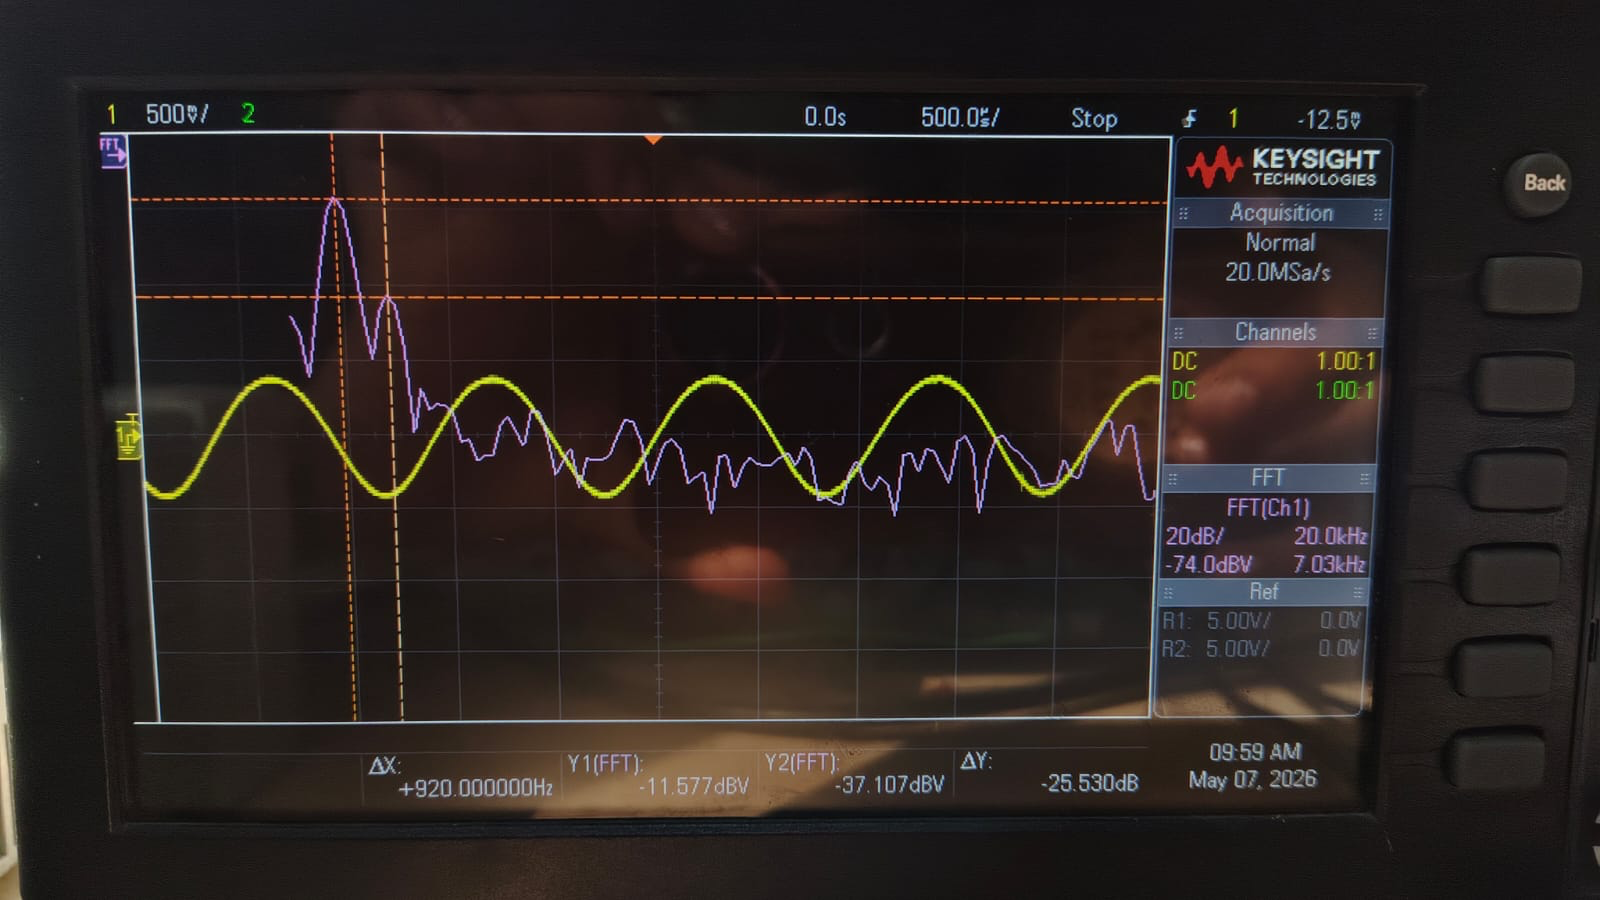
\includegraphics[width=\columnwidth]{images/5-final_sine.png}
        \caption{Final Quadrature ($Q$) Signal.}
        \label{fig:dso_final_sin}
    \end{subfigure}
    \caption{DSO Measurements of the Final Amplified I and Q Components.}
    \label{fig:dso_final_outputs}
\end{figure}

\begin{figure}[H]
    \centering
    \begin{subfigure}[b]{\columnwidth}
        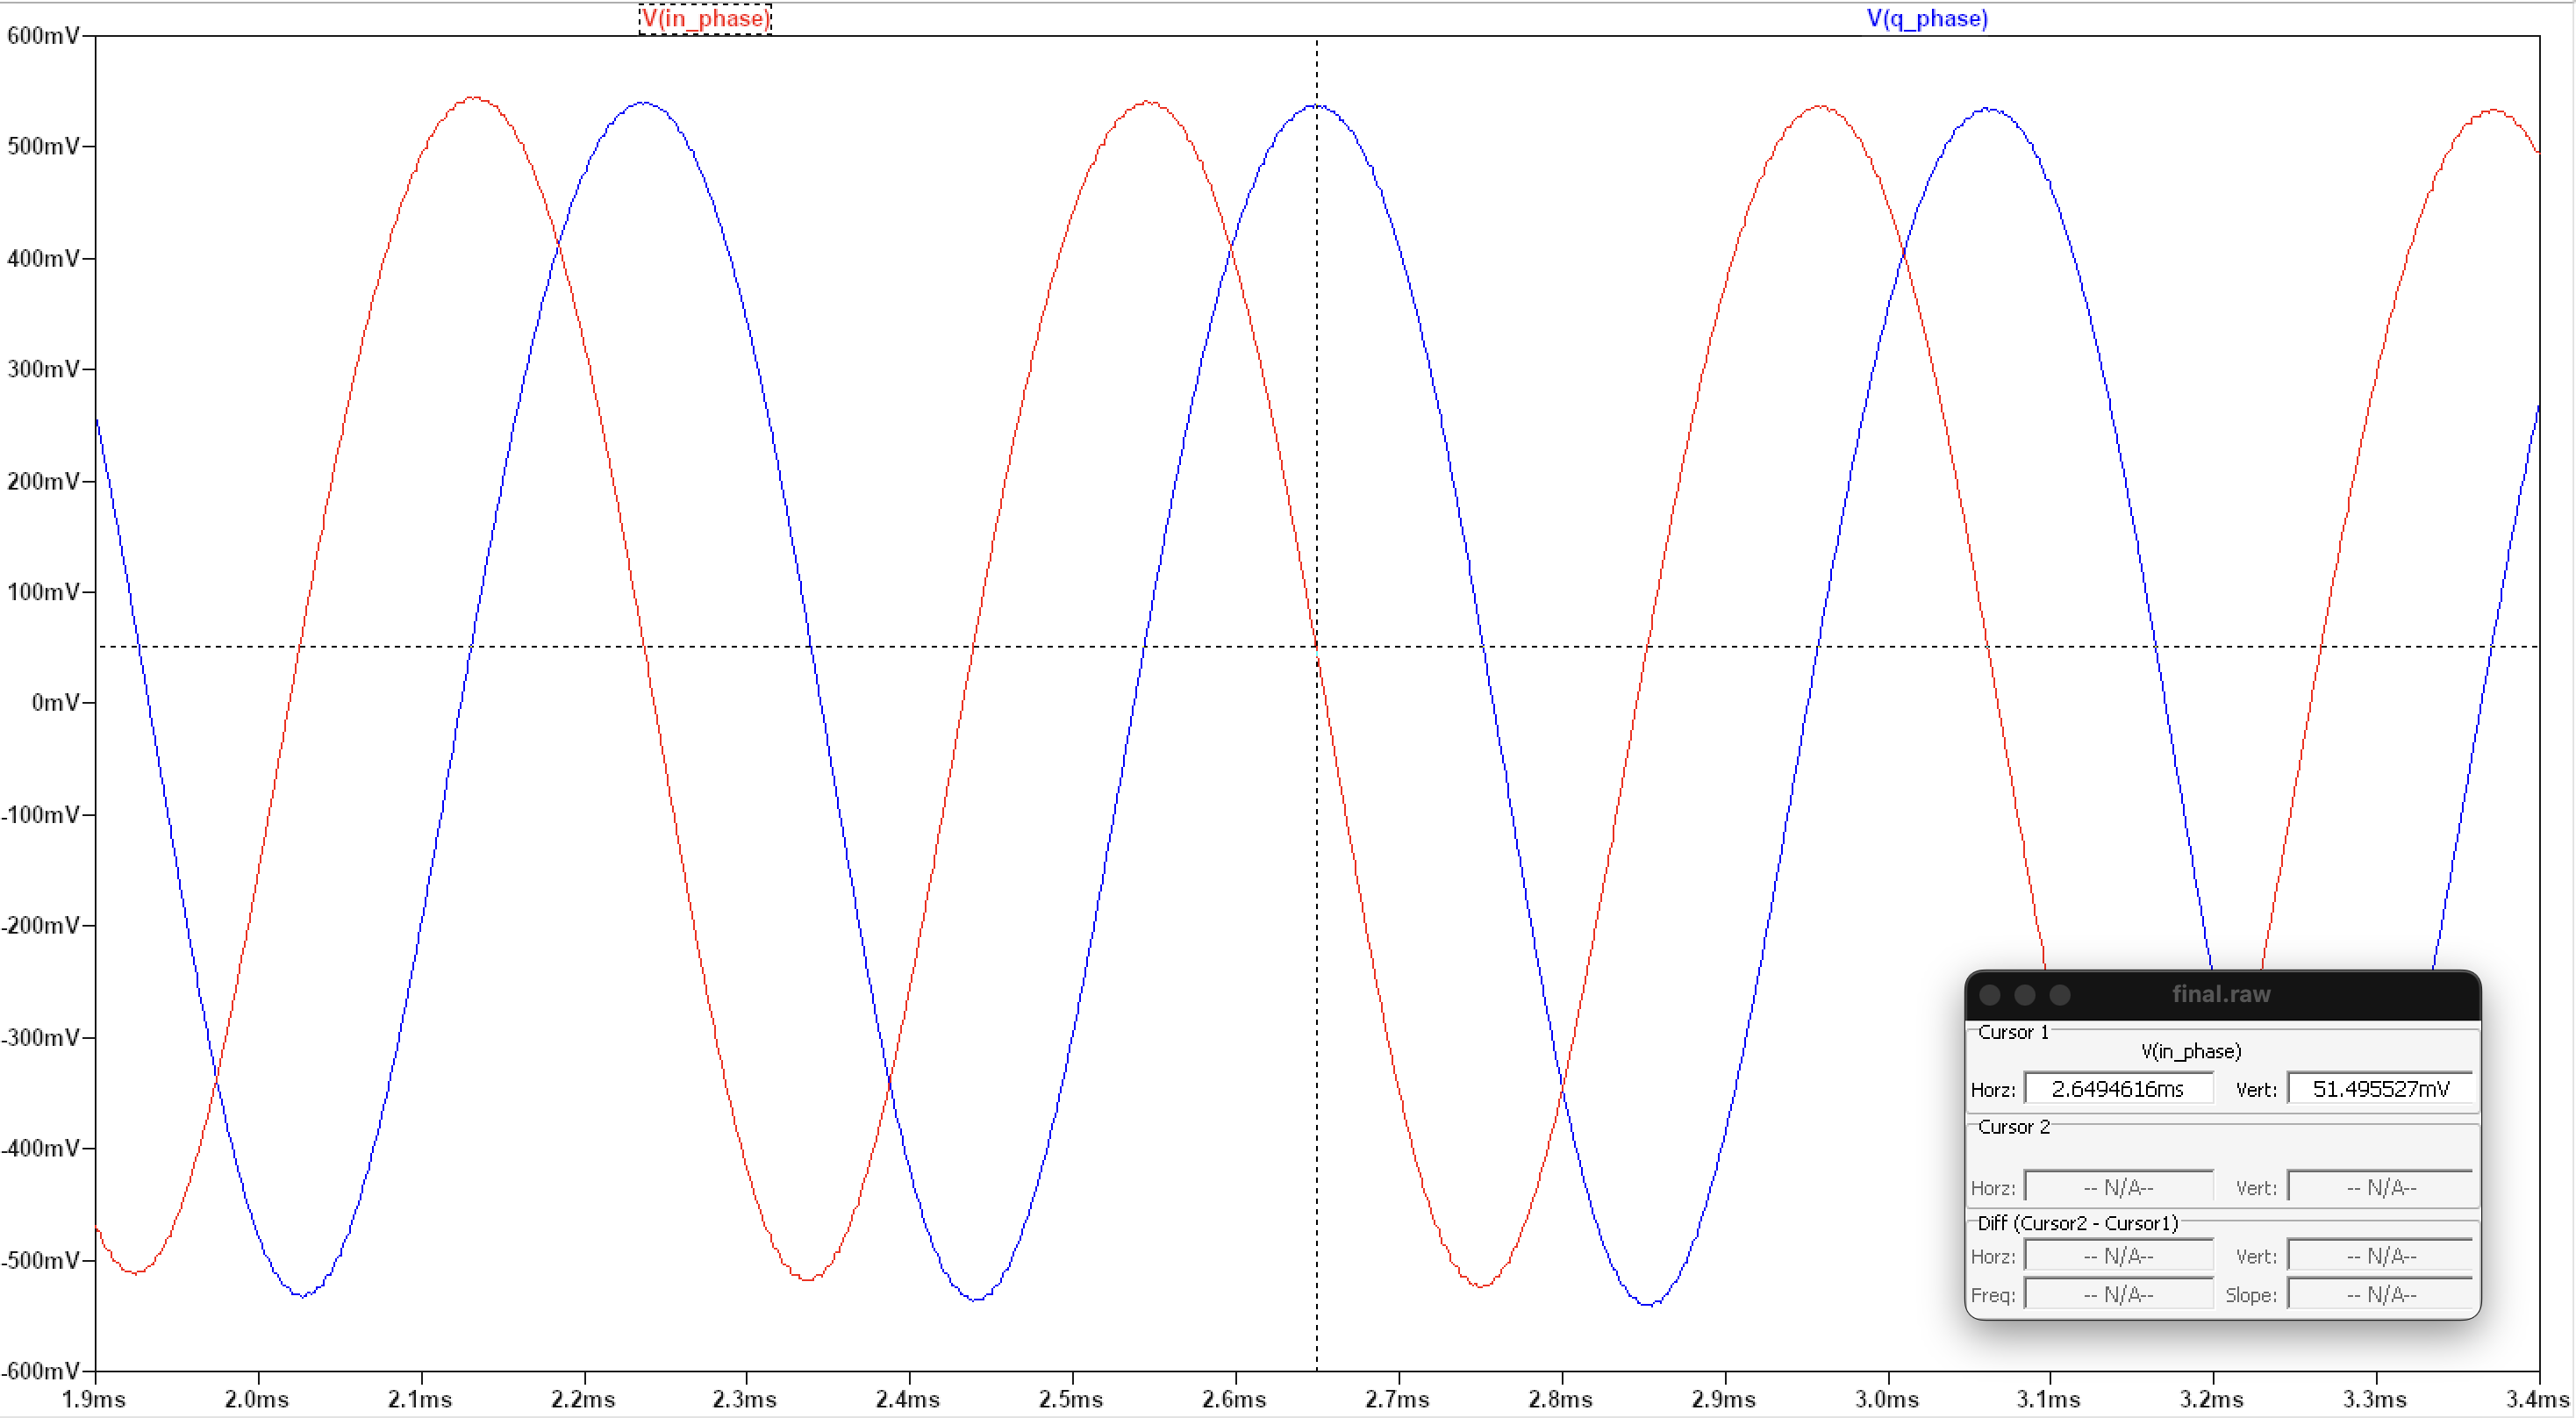
\includegraphics[width=\columnwidth]{images/5-phase-diff-iq1.png}
        \caption{Phase Difference Capture 1.}
        \label{fig:dso_phase1}
    \end{subfigure}
    
    \vspace{0.3cm}
    \begin{subfigure}[b]{\columnwidth}
        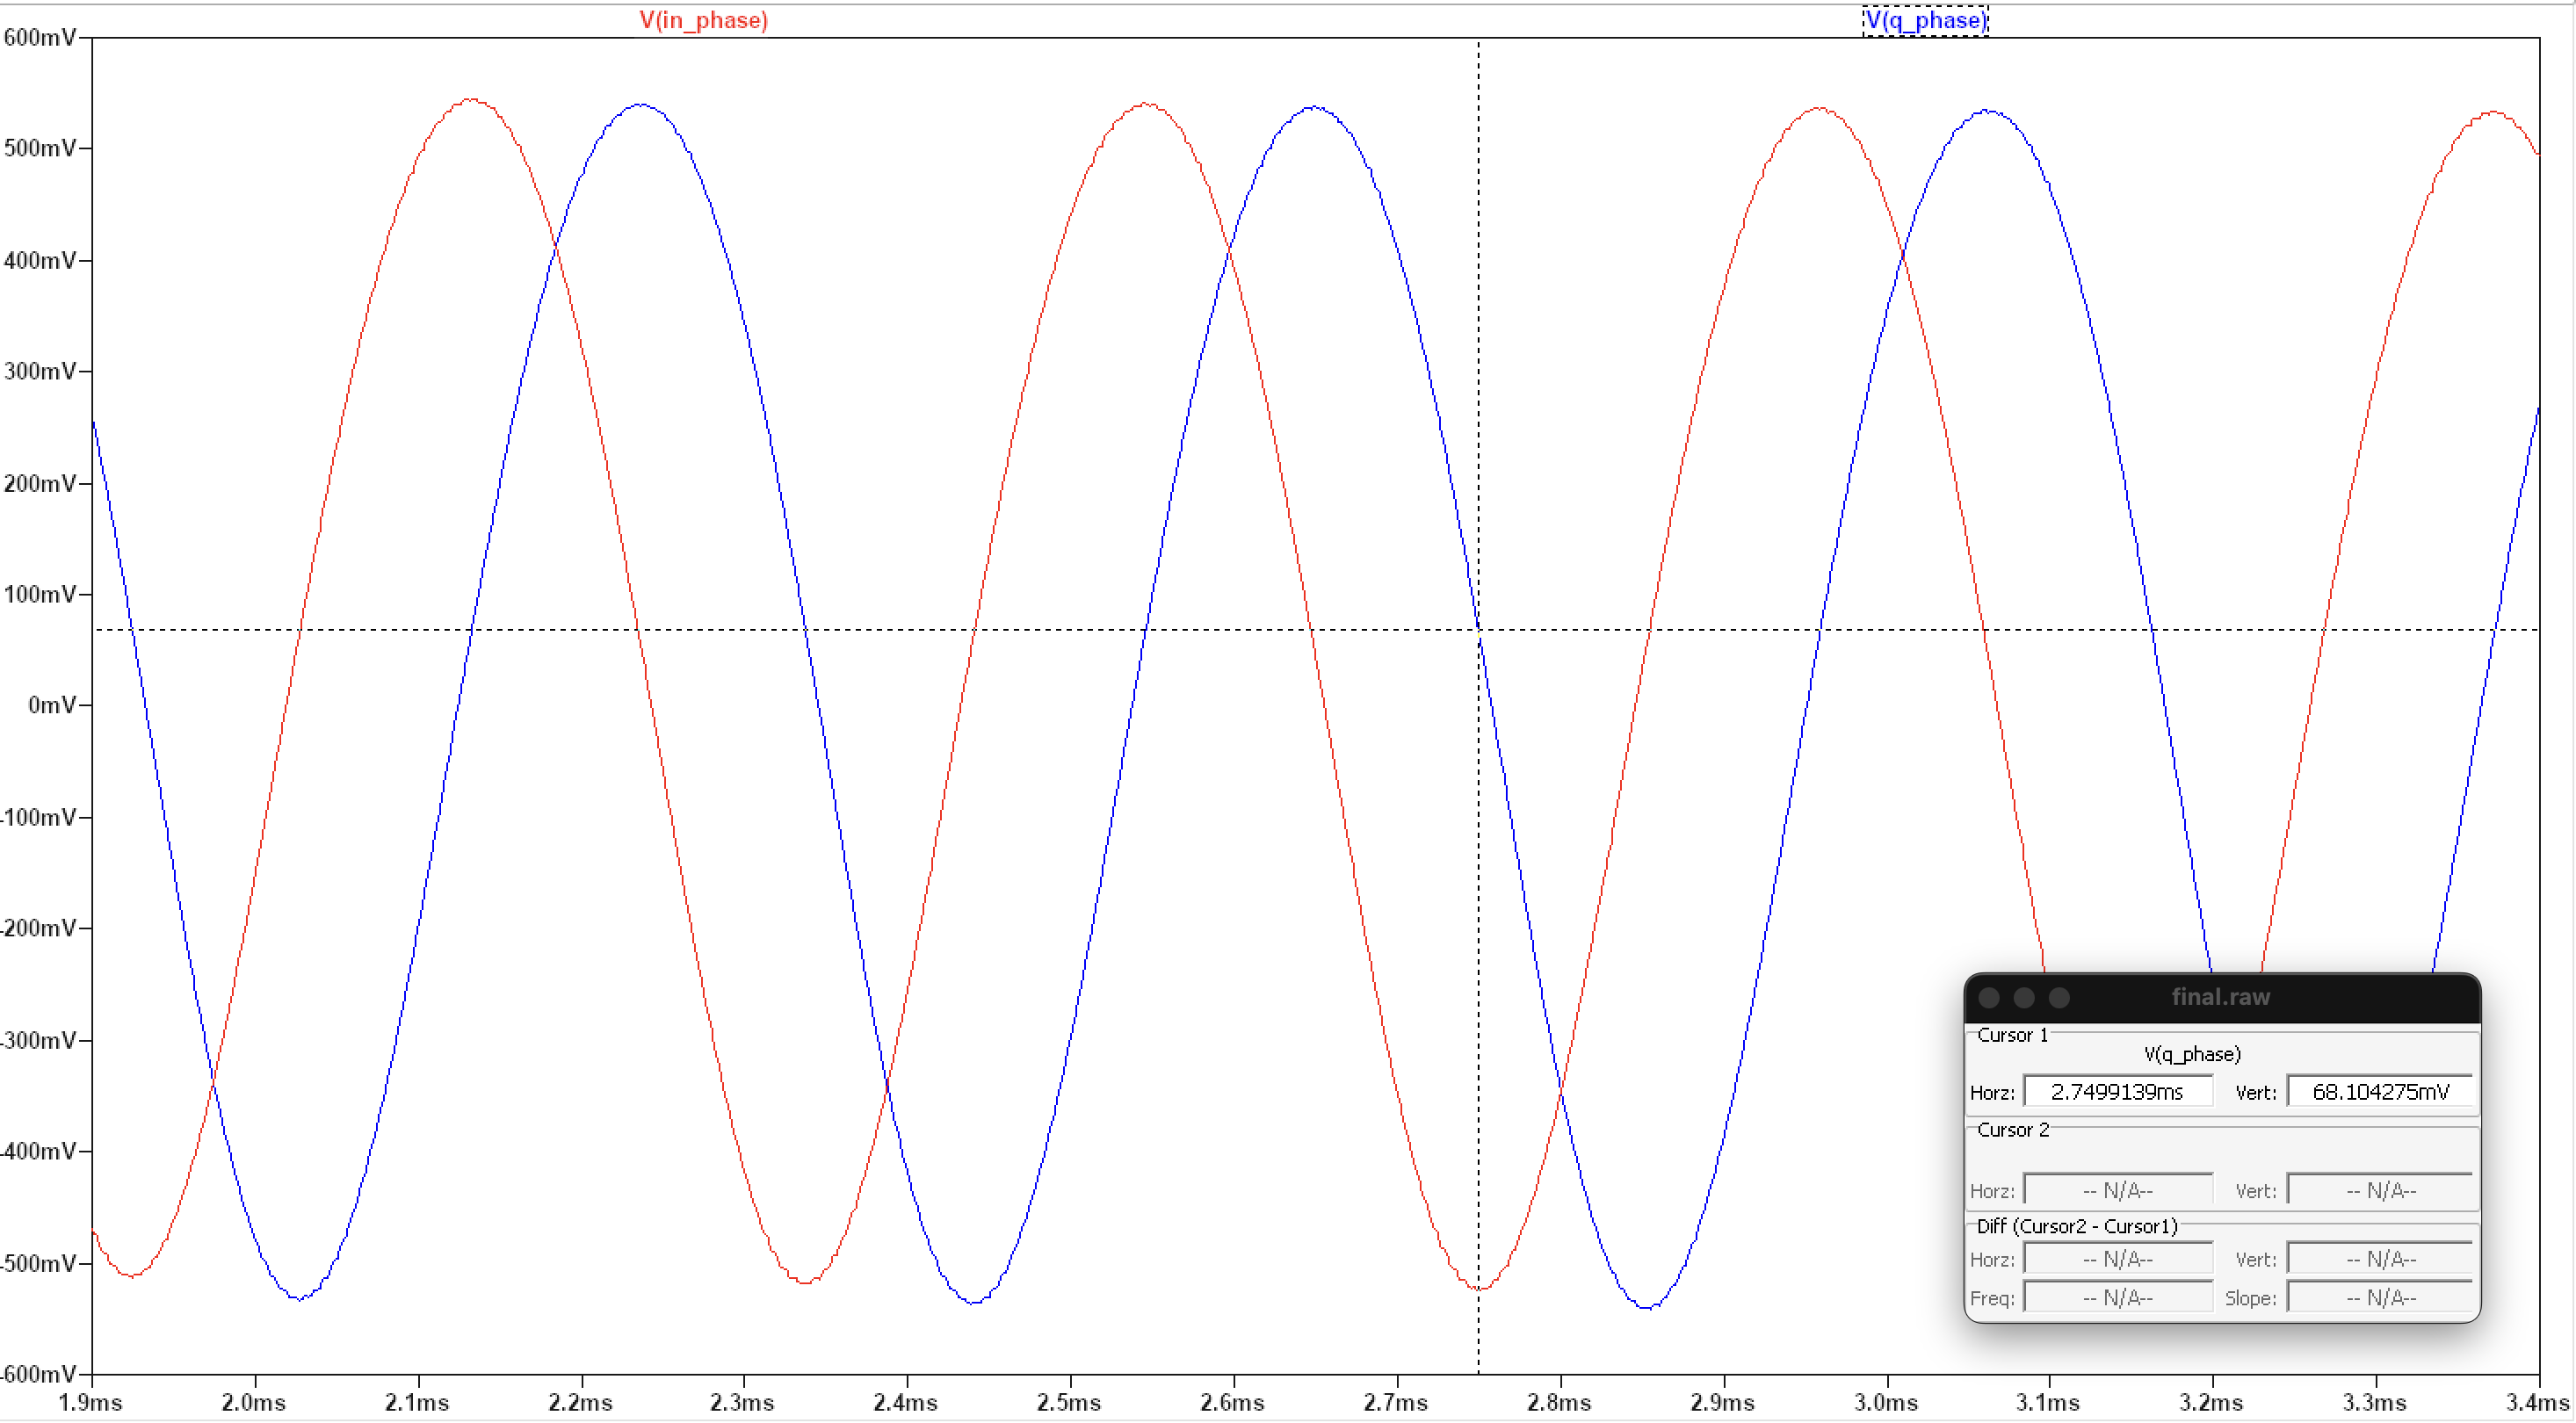
\includegraphics[width=\columnwidth]{images/5-phase-diff-iq2.png}
        \caption{Phase Difference Capture 2.}
        \label{fig:dso_phase2}
    \end{subfigure}
    \caption{DSO Measurements Verifying the $90^\circ$ I-Q Phase Shift.}
    \label{fig:dso_phase_diff}
\end{figure}

\begin{figure}[H]
    \centering
    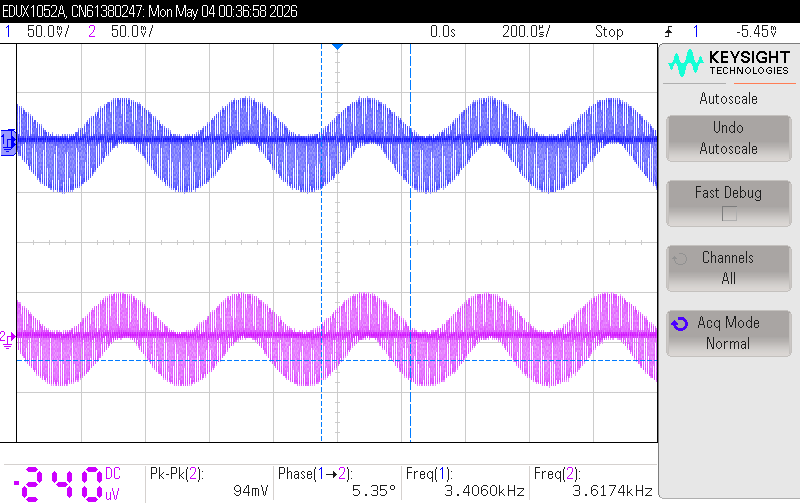
\includegraphics[width=\columnwidth]{images/mixer-ouput-both-inphase-and-quadrature-phase.png}
    \caption{Final DSO Output: In-Phase (I) and Quadrature-Phase (Q) IF Signals.}
    \label{fig:quadrature_output_dso}
\end{figure}

The hardware measurements strongly correlate with the simulation models. The final In-Phase ($I$) and Quadrature ($Q$) signals exhibit the expected $5\text{ kHz}$ frequency and robust amplified amplitude. The dual-channel DSO captures (Fig. \ref{fig:dso_phase_diff}) unequivocally verify the critical $90^\circ$ phase relationship between the two paths, proving that the quadrature architecture functions as a reliable analog downconverter.

\subsection{Performance Summary and Comparison (Q5(e))}
A comprehensive comparison between the LTSpice simulation results and the physical laboratory measurements is detailed in Table \ref{tab:performance_comparison}. The measured parameters closely align with theoretical expectations, with minor deviations attributed to component tolerances and non-ideal hardware parasitics.

\begin{table}[H]
\centering
\caption{Performance Summary and Comparison}
\renewcommand{\arraystretch}{1.3}
\begin{tabular}{|l|c|c|}
\hline
\textbf{Parameters} & \textbf{Simulated} & \textbf{Measured} \\
\hline
Oscillator Frequency & $200\text{ kHz}$ & $174\text{ kHz}$ \\
\hline
Oscillator Amplitude (I-phase) & $500\text{ mV}_{\text{peak}}$ & $430\text{ mV}_{\text{peak}}$ \\
\hline
Oscillator Amplitude (Q-phase) & $500\text{ mV}_{\text{peak}}$ & $515\text{ mV}_{\text{peak}}$ \\
\hline
Input frequency & $202\text{ kHz}$ & $171\text{ kHz}$ \\
\hline
IF & $\text{2 kHz}$ & $3\text{ kHz}$ \\
\hline
Supply & $\pm 15\text{ V}$ & $12\text{ V}$ \\
\hline
$V_{BIAS}$ & $1.2\text{ V}$ & $1.2\text{ V}$ \\
\hline
$C_C$ & $10\text{ nF}$ & $10\ \mu\text{F}$ \\
\hline
Phase Difference (I vs Q) & $93^\circ$ & $85^\circ$ \\
\hline
Final IF Amplitude ($V_{IF\_FINAL}$) & $1.3\text{ V}$ & $800\text{ mV}$ \\
\hline
LPF Resistor ($R$) & $4.7\text{ k}\Omega$ & $2.2\text{ k}\Omega \times 2$ \\
\hline
LPF Capacitor ($C$) & $10\text{ nF}$ & $10\text{ nF} \times 2$ \\
\hline
\end{tabular}
\label{tab:performance_comparison}
\end{table}

\section{Conclusion}
This report successfully outlines the theoretical foundation and implementation parameters of a Quadrature Down Converter. Mathematical derivations confirm the $90^\circ$ phase shift generated by the oscillator's topology and calculate precise component values for a $170\text{ kHz}$ oscillation frequency. Lab methodologies, including the cascaded LPF for steeper roll-off and a final CE BJT amplifier for reaching the precise $400\text{ mV}_{\text{pp}}$ amplitude requirement, were theoretically justified, ensuring the circuit acts as a robust frequency downconverter.

\begin{thebibliography}{00}
\bibitem{holzel} R. Holzel, ``A Simple Wide-Band Sine Wave Quadrature Oscillator,'' \textit{IEEE Transactions on Instrumentation and Measurement}, vol. 42, no. 3, pp. 758--760, Jun. 1993.
\bibitem{abidi} A. A. Abidi, ``Direct-conversion radio transceivers for digital communications,'' \textit{IEEE Journal of Solid-State Circuits}, vol. 30, no. 12, pp. 1399--1410, Dec. 1995.
\bibitem{razavi} B. Razavi, \textit{RF Microelectronics}, 2nd ed. Upper Saddle River, NJ, USA: Prentice Hall, 2011.
\end{thebibliography}

\end{document}
